\chapterimage{Detector/DetFigures/VirgoTube.jpg} % Chapter heading image
%Einstein Telescope artist impression, copyright Nikhef
\chapter{Detector}
\label{chap:Detector}

%**********************************************
\section {Optical Layout}
% Authors A. Freise, S. Hild
\label{Sec:Layout}

\FloatBarrier
\label{sec:optlayout}

\tcb{from ET design  1.3.1}

\begin{wrapfigure}{r}{0.4\textwidth}
%\begin{figure}{H}
	\centering
		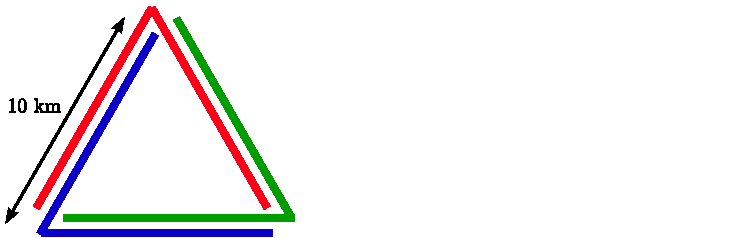
\includegraphics[width=0.3\textwidth]{Detector/Optics/Images//NestedDetectors.pdf}
	\caption{Three nested detectors in a triangular arrangement will 
	form the final Einstein Telescope geometry.}
	\label{fig:NestedDetectors}
\end{wrapfigure}
In its final construction stage the Einstein Telescope will consist of three nested detectors, which will be arranged in a triangular pattern as shown in figure\,~\ref{fig:NestedDetectors}. In contrast to the traditional L-shaped geometry of the first and second generations of gravitational wave detectors this arrangement is equally sensitive for both polarisations of the gravitational wave. Additionally it shows a more isotropic antenna pattern compared to the L-shaped detectors, as shown in figure\,~\ref{fig:response}. The overall frequency range covered will reach from a few Hertz to about 10\,kHz.

Each individual detector in turn will comprise two interferometers, one specialised for detecting low-frequency gravitational waves and the other one for the high-frequency part. The sensitivity goal for each interferometer is shown in figure\,\ref{fig:ET_sensitivity}. %\\ 
Each individual interferometer has a classical dual-recycled Michelson topology with arm cavities. This is a mature technique, well tested in laboratory experiments, and currently being set up for the second-generation detectors, Advanced LIGO and Advanced Virgo. More elaborate topologies like Sagnac interferometers or optical bars using Quantum Non-Demolition (QND) techniques do not promise significant advantages and have not yet reached the level of  maturity required for a project of this scale.\\



\tcb{from ET design  5.4}
This section describes the details of the ET optical layout, such as the laser beam sizes, beam shapes and distances between optical components inside the arm cavities and central interferometer including the power and signal recycling cavities. A schematic sketch of the optical layout of all core optical of the interferometers is shown in figure~\ref{Fig:Simple_ETv1}.
Constraints imposed onto the optical layout are briefly discussed in section~\ref{sec:opt_layout_class}, while  section~\ref{sec:xylophone} lays out the motivation for choosing a dual-tone xylophone detector. The optical layout of the arm cavities is discussed in detail in section~\ref{sec:arm_cavity_design}. Finally section~\ref{sec:opt_layout_CITF} describes the layout of the recycling cavities. 

\begin{figure}[p]
\centering
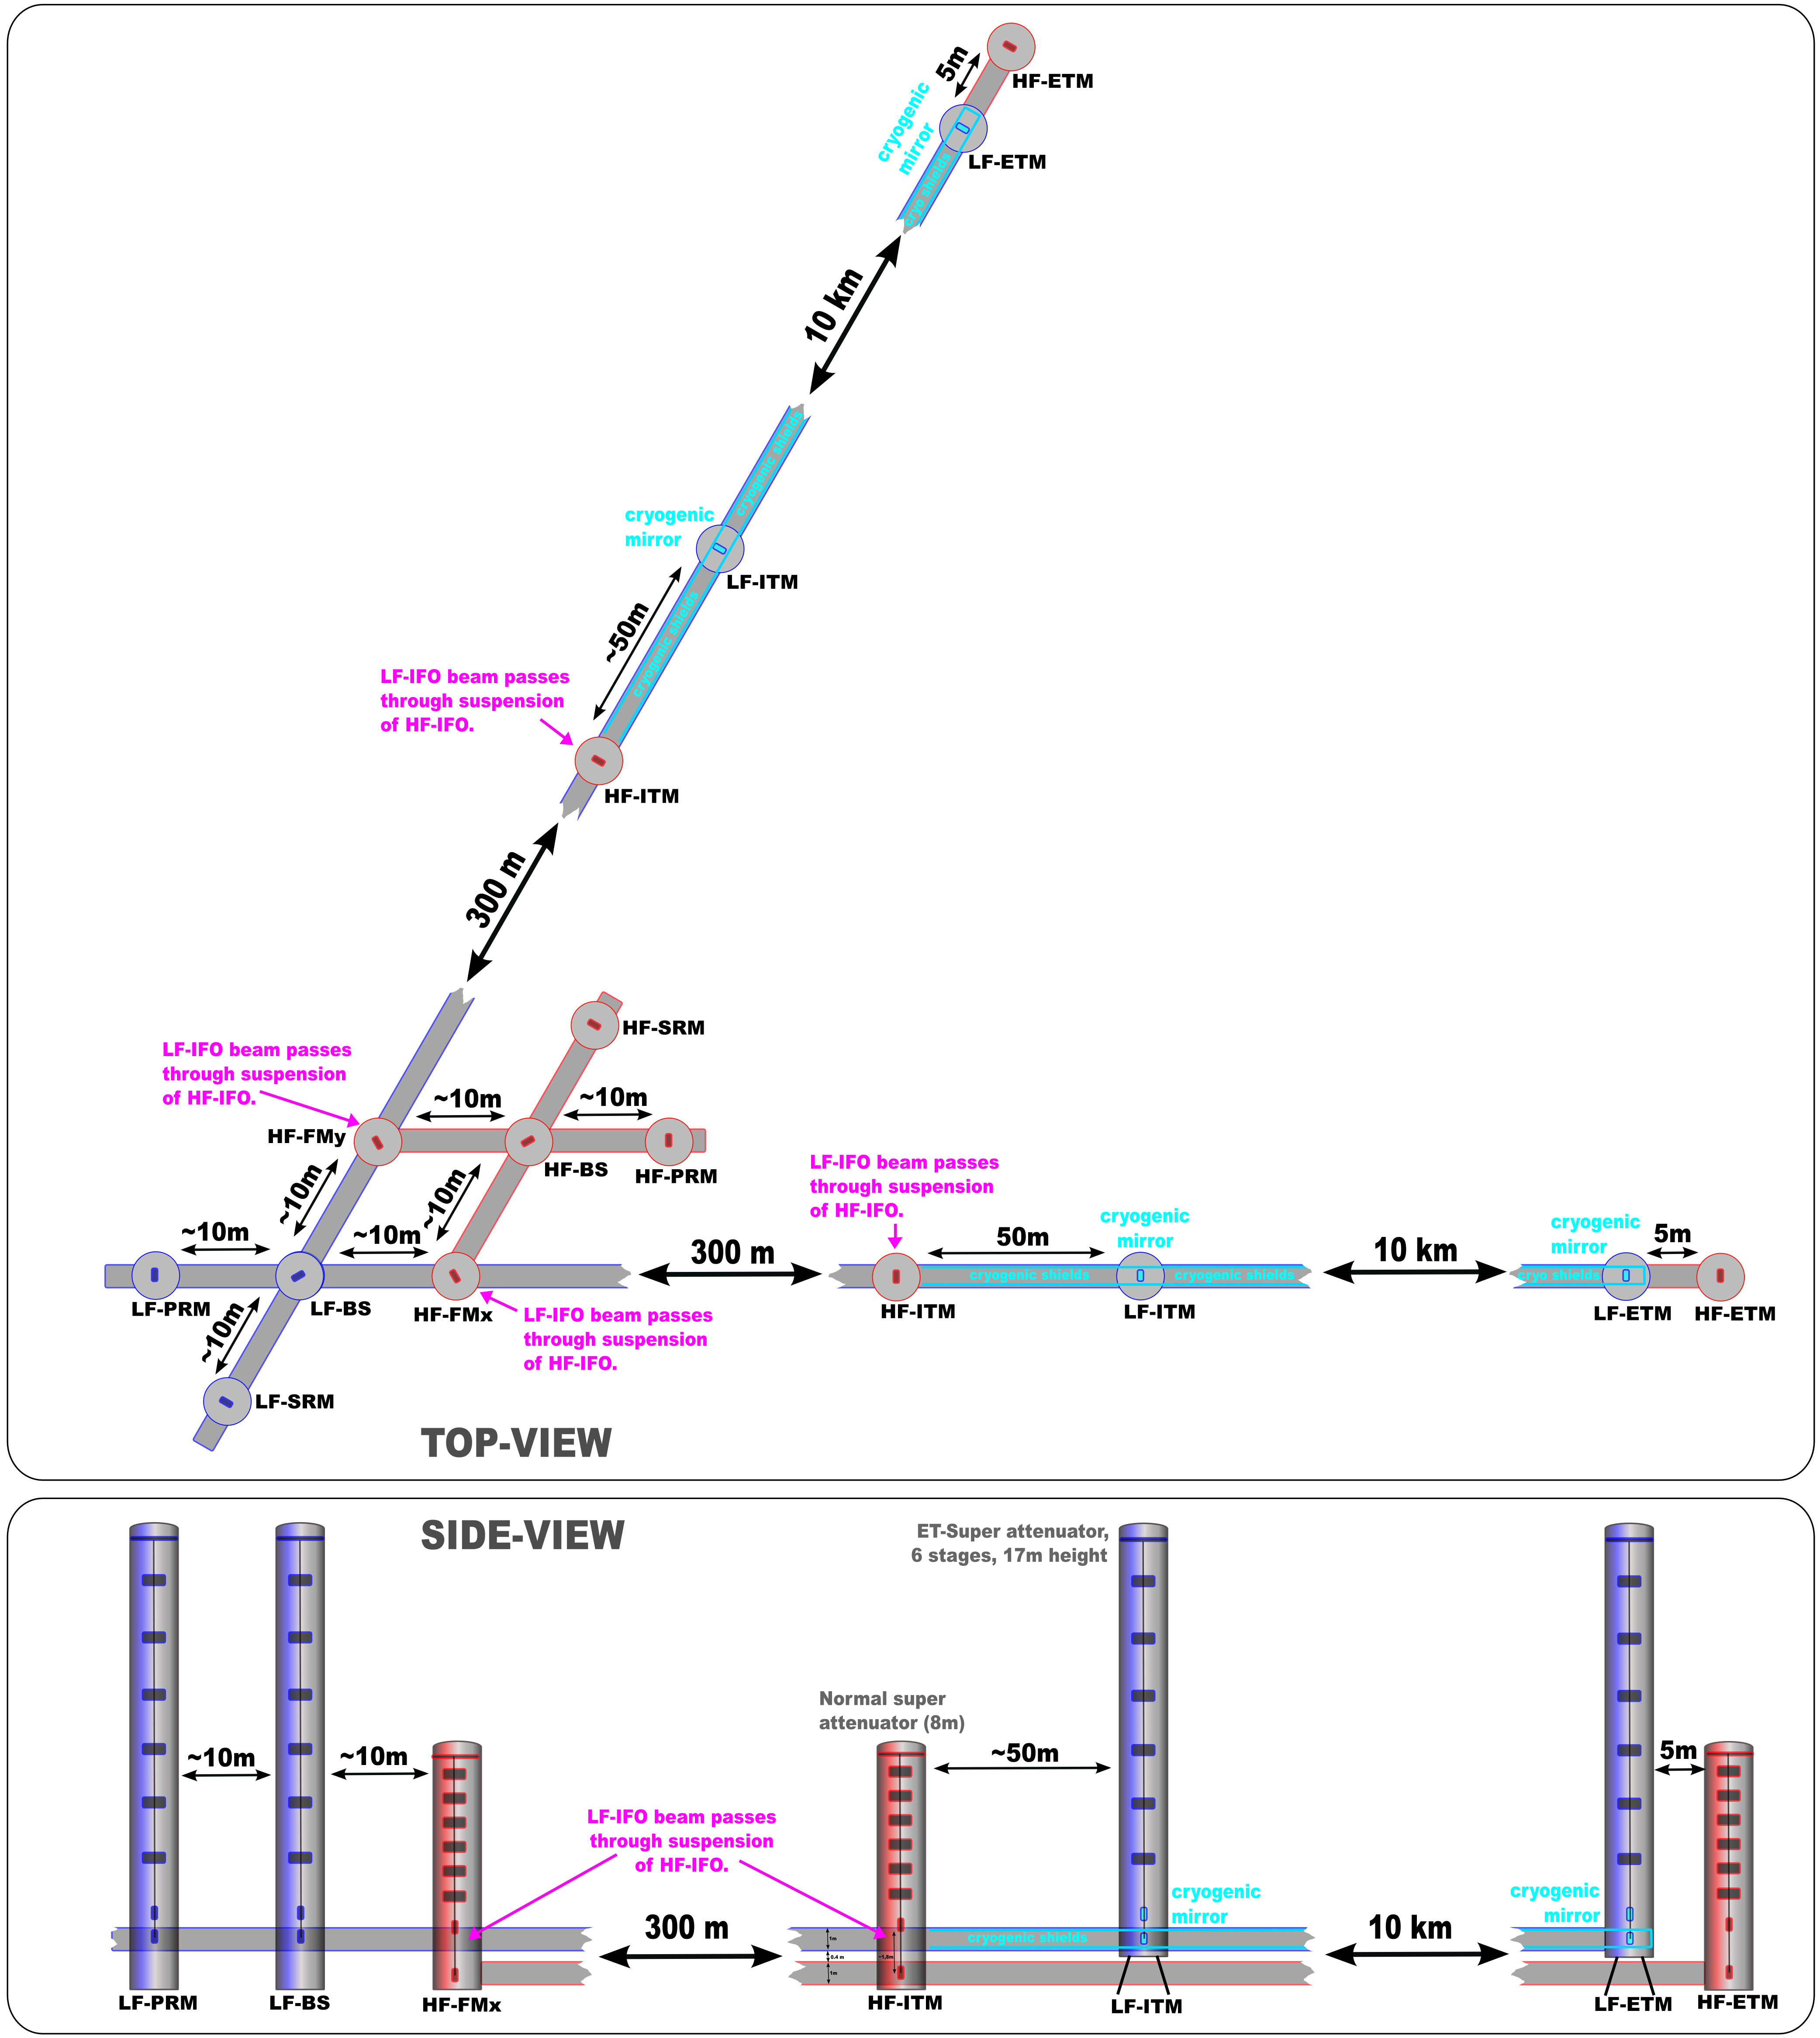
\includegraphics[width=1\textwidth]{Detector/Optics/Images/ET_April2011_v2.png}
\caption{Simplified drawing of the low and high frequency core interferometers of a single ET-detector. Injection and detection optics as well as filter cavities have been omitted for clarity. Please not that the complete ET observatory consists of three such detectors.%
}
\label{Fig:Simple_ETv1}
\end{figure}

\subsubsection{A xylophone design for ET}\label{sec:xylophone} 
\tcb{from ET design  5.4.2}
Spanning the detection band over four orders of magnitude in frequency, as is asked for third generation GW observatories such as ET, is technically extremely challenging: different noise types dominate the various frequency bands and often show opposite responses for different tuning of the same design parameter.

In the following we give some examples of fundamental issues of a broadband third generation interferometer that could be resolved by using a set of xylophone detectors:
\begin{itemize}
\item \textbf{High Power vs Cryogenic Temperature}: Using a single broadband ET observatory as described in \cite{HildETconventional} features the challenge of the simultaneous use of high optical power (a few megawatts) to achieve the required high frequency sensitivity and test masses at cryogenic temperatures in order to provide the required suppression of thermal noise. Even though tiny, the residual absorption of the dielectric mirror coatings deposits heat in the mirrors which is difficult to extract, without spoiling the performance of the seismic isolation systems. A possible solution for this problem would be to build a xylophone observatory consisting of a high frequency detector featuring high power and high temperature and a low frequency detector featuring low power and cryogenic temperatures.
\item \textbf{Shot Noise vs Radiation Pressure Noise}: Due to the fact that the shot noise contribution scales inverse with optical power, but the photon radiation pressure noise contribution on the other hand  scales proportional to the optical power, it will be hard to obtain the desired bandwidth with a single detector. Therefore, again it might be useful to split ET into a low-power low-frequency and a high-power high-frequency
companion.
\item \textbf{Mixing Interferometer Topologies}: Xylophone configurations would also allow us to mix alternative interferometer topologies, such as Sagnac interferometer \cite{Chen2003} and optical levers \cite{Khalili2002}, with the standard Michelson interferometer. For example one could imagine that ET upgrades would feature a standard high-frequency Michelson interferometer with a low-frequency optical lever as companion.
\end{itemize}

The xylophone concept was first suggested for Advanced LIGO,  proposing to complement the standard broadband interferometers with an interferometer optimized for lower frequency, thus enhancing the detection of high-mass binary systems
\cite{Shoemaker2001LIGOXylophone, Conforto2004}.

One may think that a xylophone might significantly increase the required hardware and its cost by the need to build more than one broadband instrument. However, such an argument does not take the technical simplifications that it would allow, the better reliability of simpler instruments, and the more extensive scientific reach allowable into account.

For example splitting a third generation observatory into a low-power, low-frequency  and a high-power high-frequency interferometer, has not only the potential to resolve the above mentioned conflict of photon shot noise  and photon radiation pressure noise, but also allows to avoid the combination of high optical power and cryogenic test masses. To reduce thermal noise to an acceptable level in the low frequency band, it is expected that cryogenic suspensions and test masses are required. Even though tiny, the residual absorption of the dielectric mirror coatings deposits a significant amount of heat in the mirrors. Since this heat is difficult to extract, without spoiling the performance of the seismic isolation systems, it imposes a limit on the maximum circulating power of a cryogenic interferometer.

\begin{figure}[thbp]
\centering
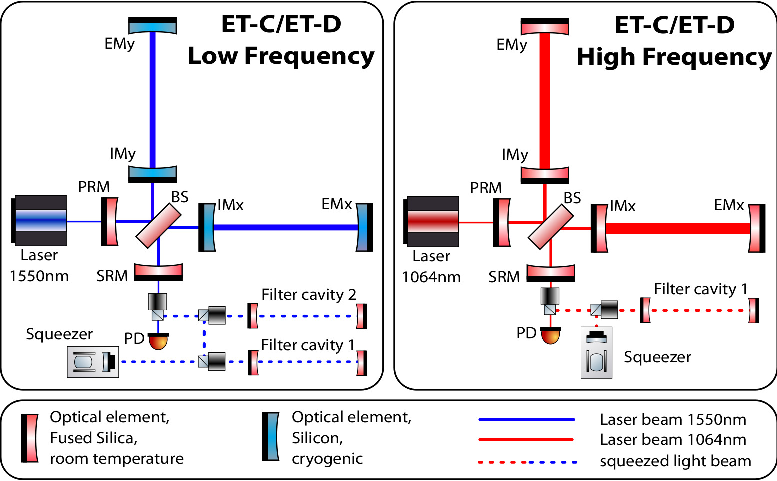
\includegraphics[width=0.8\textwidth]{Detector/Optics/Images/Layout_overview.pdf}
\caption{Simplified sketch of the ET low and high frequency core interferometers of a single ET-detector.}
\label{Fig:opt_lay_over}
\end{figure}

\begin{table}
\begin{center}
\begin{tabular}{l l l}
\hline
\hline
Parameter & ET-D-HF   & ET-D-LF \\
\hline
Arm length & 10\,km & 10\,km \\
Input power (after IMC) & 500\,W & 3\,W \\
Arm power & 3\,MW & 18\,kW\\
Temperature & 290\,K &  10\,K  \\
Mirror material & fused silica & silicon \\
Mirror diameter / thickness & 62\,cm / 30\,cm & min 45\,cm/ T \\
Mirror masses & 200\,kg & 211\,kg \\
Laser wavelength & 1064\,nm & 1550\,nm \\
SR-phase & tuned (0.0) & detuned (0.6)\\
SR transmittance & 10\,\% & 20\,\% \\
Quantum noise suppression &  freq.\ dep.\ squeez.& freq.\ dep.\ squeez.\\
Filter cavities & $1 \times 10\,$km  & $2 \times 10\,$km\\
Squeezing level  & 10\,dB (effective) & 10\,dB (effective) \\
Beam shape &  LG$_{33}$& TEM$_{00}$\\
Beam radius & 7.25\,cm & 9\,cm \\
Scatter loss per surface & 37.5\,ppm & 37.5\,ppm \\
Seismic isolation & SA, 8\,m tall & mod SA, 17\,m tall \\
Seismic (for $f>1$\,Hz) & $5\cdot 10^{-10}\,{\rm m}/f^2$ & $5\cdot 10^{-10}\,{\rm m}/f^2$  \\
Gravity gradient subtraction & none & none \\
\hline
\hline
\end{tabular}
\caption{Summary of the most important parameters of the ET-D high and low frequency interferometers. SA~=~super attenuator,  freq.\ dep.\ squeez.~=~squeezing with frequency dependent angle.\label{tab:summary14}}
\end{center}
\end{table}

The baseline for ET is a 2-band xylophone detector configuration, composed of a low-frequency (ET-LF) and a high-frequency (ET-HF) detector. Both interferometers are Michelson interferometers featuring 10\,km armlength and an opening
angle of 60 degrees.  Due to their similar geometry both detectors will share a single facility. Table~\ref{tab:summary14} gives a brief overview of the main parameters of the analysed low-frequency (ET-LF) and high-frequency (ET-HF) detector. Figure~\ref{Fig:opt_lay_over}   shows sketches of the corresponding core interferometers and the filter cavities. The full layout of the two core interferometers of a single ET detector is depicted in Figure~\ref{Fig:Simple_ETv1}.


% -------------------------------------------------------------------------------------------
\subsubsection{Arm cavity design}
\label{sec:arm_cavity_design}
\tcb{from ET design  5.4.3}

The size and shape of the laser beam inside the interferometer is defined by the surface shape of the cavity mirrors; the beam sizes at the arm cavity input mirrors (IM) and arm cavity end mirrors (EM) as well as the position of the cavity waist are determined by only two parameters, the radii of curvature (ROC) of IM and EM. Since inside the two Fabry-Perot cavities of the Michelson interferometer the GW interacts with the laser light, creating signal sidebands, the two arm cavities can be seen as the heart of the ET interferometers. The characteristics of the arm cavities have not only a high impact on the detector sensitivity and bandwidth, but also on the overall detector performance.

The choice of the beam size on the arm cavity mirrors is a trade-off process taking the following considerations into account:
\begin{itemize}
  \item For a given cavity length there is a minimal achievable beam size, which is determined by the divergence of the beam.
\item Above this minimal beam size, any further increase in beam size leads to and additional reduction of the various thermal noise contributions.
\item Finally the upper limit for the manageable beam size is given firstly by the maximum available mirror substrate size and secondly by the approaching of the cavity instability.
\end{itemize}

\textbf{Arm cavity mirror size}

A common method to define the mirror size is to demand the optical power loss due to clipping (light being lost because it `falls over the edge of the mirror') to be less than $1\,$ppm. The computation of the scaling factors is described in~\cite{Chelkowski2009} and results in:
\begin{center}
\begin{tabular}{|l|c|c|}
	\hline
	mode  & TEM$_{00}$ & LG$_{33}$\\
	\hline
	mirror radius to beam  radius & 2.63 & 4.31\\
	\hline
\end{tabular}
\end{center}

\textbf{Minimal mirror sizes for ET}

Using the currently discussed options for ET we can compute minimal mirror sizes for various options, by using $L=R_{C}$ resulting in $w_{\rm min}=\sqrt{\frac{L\lambda}{\pi}}$.
\begin{center}
\begin{tabular}{|l|c|c|}
	\hline
setup & min beam radius  & min mirror diameter \\
         & [cm] & [cm] \\
	\hline
LG$_{33}$, 1064\,nm  &  5.8      &  50.2     \\
	\hline
TEM$_{00}$, 1550\,nm  &  7.0      &   37.0    \\
	\hline
\end{tabular}
\end{center}

\textbf{Realistic mirror sizes for ET}

Using the minimal beam sizes is obviously not optimal in terms of thermal noise. Therefore we intend to push the beam sizes for ET towards the maximum feasible size, which corresponds to about 60\,cm substrate diameter for fused silica mirrors and 50\,cm for the silicon mirrors. Assuming 10\,km long arm cavities, we can derive the following arm cavity characteristics.

\begin{center}
\begin{tabular}{|c|c|c|c|c|c|c|c|c|}
  \hline
IFO & $\lambda$& beam shape & mirror diameter & $R_{\rm C}$ & $w_0$ &$z_0$ & $w$ & $z_{\rm R}$ \\
\hline
ET-HF & 1064\,nm & LG$_{33}$ & 62\,cm & 5691\,m & 2.51\,cm & 5000\,m & 7.2\,cm & 1859\,m\\
\hline
ET-LF & 1550\,nm & TEM$_{00}$ & 45\,cm &5577\,m & 2.9\,cm & 5000\,m & 9.0\,cm & 1698\,m\\
\hline
\end{tabular}
\end{center}

% ----------------------------------------------------------------------------------------------------

\FloatBarrier
\subsubsection{Central interferometer design}
\label{sec:opt_layout_CITF}
\tcb{from ET 5.4.4 design}

The central interferometer consists of the two recycling cavities and the central Michelson interferometer formed by the beam splitter and the arm cavity input mirrors. The design of the central interferometer is mainly determined by two constraints. First of all it should allow for the implementation of non-degenerate recycling cavities. Second, the central interferometer has to serve as mode-matching telescope for the arm cavities.

The non-degenerate recycling cavity design used by the advanced detectors (see Figure~\ref{Fig:Sec_Optics_AdvLIGO_IFO_Schematic}) can probably not be directly adapted for ET, because no beam splitter substrates of the required dimensions would be available. For example the high frequency interferometer featuring an opening angle of  60 degree would require a beam splitter with a diameter of 115\,cm.

Therefore we plan to investigate design options making use of input mirror substrates including a focussing lens with a focal length of 0.2 to 1\,km and shifting the input mirrors away from the beam splitter.  Figure~\ref{Fig:Simple_ETv1} illustrates how such a configuration would look like. Please note that the arm cavity mirrors are the only full sized optical elements and that beam splitter and recycling mirrors can be significantly smaller. In addition in this scenario no additional folding mirrors are necessary in the recycling cavities.

\textbf{Layout option for TEM$_{00}$, 1550\,nm}
\nopagebreak

The optical parameters of a possible solution based on a arm cavity length of $L=10$\,km and a TEM$_{00}$ mode at 1550\,nm are provided below:
\begin{itemize}
\item focussing element in or near the ITM with a focal length of $f=303$\,m
\item distance ITM--BS: 300\,m
\item distance BS--MPR: 10\,m
\item beam size on BS: 6\,mm
\item beam size on MPR: 3.4\,mm
%\item Rayleigh range in central interferometer: 6.3\,m
\end{itemize}

The recycling cavity formed by MPR and ITM has a length of 310\,m and a free spectral range of 484\,kHz. The round-trip Gouy phase is given by $\approx 9.6$\,deg which corresponds to a mode separation frequency of $25.8$\,kHz.

\textbf{Layout option for LG$_{33}$, 1064\,nm}
\nopagebreak

Using the same distances and focussing elements for the interferometer with a LG$_{33}$, 1064\,nm beam, we also obtain reasonable numbers:
\begin{itemize}
\item beam size on BS: 4.7\,mm
\item beam size on MPR: 2.7\,mm
%\item Rayleigh range in central interferometer: 6.7\,m
\item Gouy phase: 10.5\,deg
\item mode separation frequency:  28.1\,kHz
\end{itemize}

These layout options are not yet optimised but they show that a separation between beam splitter and input optics in the order of 300\,m represents a useful baseline. The numbers for the beam sizes at the beam splitter and recycling mirrors in both cases need to be checked against a detailed thermal noise computation.

Furthermore, the design needs to be evaluated for losses originating from astigmatisms inside the recycling cavities as well as for scattered noise issues.





\FloatBarrier
\section{Optics and Interferometry}
% Authors R.Flaminio, A. Freise, S.Hild
\label{Sec:Optics}

\subsection{Core Optics and Coatings}
%  Author: Jerome
\label{Sec:CoreOptics}
This section focuses on the mirrors forming the arm cavities of the interferometer (IM and EM). Those optics, also called test masses, are the largest \tcb{(comment sthild:) by dimension} and most critical ones whose displacement noise can directly degrade the  \tcb{(comment sthild:) measurement of the } gravitational waves signals.

To ensure the best optics, the three ingredients of a mirror: substrate, polishing and coating will have to use state of the art technologies. An overview of current achievements and the core optics strategy for ET is presented in the following sections. The working temperature of the optics \tcb{(comment sthild:) better say "The temperature at which the mirror is operated  has ..." } have a strong impact on the technological choices to be made. 

\subsubsection{The substrate materials}

The substrate of the large \tcb{(comment sthild:) replace 'large' by 'ET main' } optics must meet some drastic \tcb{(comment mlorenzini: replace specifications with requirements)} specifications in term\tcb{s} of optical and mechanical specifications, moreover it should be available in large sizes with surfaces polished to the atomic level. Due to such constraints, \tcb{(comment sthild:) only a }few specific materials can be considered: fused silica for room temperature interferometer and silicon for cryogenic temperatures.\\

\paragraph{Fused silica} is the substrate of choice for all the current room temperature interferometers.  Due to its \tcb{(comment mlorenzini: Remove 'extensive') } extensive
use for first and second generation gravitational wave detectors, this material has been extensively characterised at room temperature. Moreover the polishing and coating are now well mastered for this material \cite{pinard2017mirrors}.

The operating wavelength of room temperature ET will be 1064~nm, the same as current advanced interferometers and well within the transparency region of fused silica. At this wavelength fused silica exhibits very low bulk optical absorption (below 1 ppm/cm) with high homogeneity of refractive index (relative optical path length < 0.1~nm/cm over the central part) and very low birefringence (around 1~nm/cm \cite{Degallaix:Large_optics_19}). The material can be isotropic in 3 dimensions which is ideal for the central beansplitter where laser beams are crossing the substrate at different angles.

In addition to its outstanding optical properties, fused silica presents a very low Brownian thermal noise at room temperature. Additionally, there exist techniques to fabricate quasi-monolithic suspensions based on pulled fused silica fibres and silicate bonding to further reduce the suspension thermal noise. These techniques have demonstrated their reliability and performances for years in the GEO600 detector \cite{plissi1998aspects} and so have been successfully implemented in the LIGO and Virgo detectors \cite{robertson2002quadruple,lorenzini2010monolithic}.

As a risk reduction for ET, the upgrade of Advanced Virgo, called Advanced Virgo+, will use test masses in fused silica of diameter 55~cm weighting 100~kg, that would be an essential step towards the optics for ET-HF which will be in the same material and with a diameter of 62~cm for 200~kg. 

In a nutshell, fused silica for large optical substrates presents the best optical and mechanical performances at room temperature and with very limited risks.\\


\paragraph{Silicon} is the favorite candidate material for the test masses for the cryogenic interferometer ET-LF. Compared to fused silica (and sapphire), silicon is not transparent at 1064~nm and so the operating wavelength of the detector has to be shifted to 1550~nm. 

Silicon has excellent mechanical and thermal properties and is easily available in relatively high quality due to the large market of the semiconductor industry. The coefficient of thermal expansion is zero at two special temperatures around 18~K and 125~K \cite{lyon1977siliconexpansion}. At these temperatures the contribution of thermo-elastic noise will therefore vanish. The mechanical loss of silicon has been studied by Q-factor measurements. It was experimentally shown that silicon bulk samples can reach mechanical losses as low as $1 \times 10^{-9}$ at 10~K. \cite{mcguigan1978siliconQ}.

The maximum available diameter and purity of silicon depends on the fabrication process. The two main growing processes for single crystal silicon used by the semiconductor industry are the Czochralski (CZ) and the Float Zone (FZ) methods. CZ silicon is grown from a silicon melt in a silica crucible. It results in relative large samples with a reasonable purity. The most dominant impurities in undoped CZ-grown silicon are carbon (typically 10$^{-18}$ cm$^{-3}$) and oxygen (typically up to 10$^{-19}$ cm$^{-3}$). 

In contrast, FZ silicon contains the same impurities but in much smaller concentrations (up to 10$^{-3}$ times smaller\tcb{(comment MGranata:) I would rather say "10$^{3}$ times smaller"}). During the FZ growth process, single or poly-crystalline silicon is remelted by means of inductive heating in vacuum or under an inert atmosphere. Impurities dissolve better in the melt than in the solid part. The re-crystallised material has therefore a higher purity than the initial one. By slowly sweeping the melt from one end to the other it is possible to purify in steps. The mechanism of inductive heating sets limits to the current production setups and leads to smaller available samples.

Using the CZ growth technique, silicon ingots up to 45~cm of diameter can be produced however 30~cm is still the dominant \tcb{(comment mlorenzini: perhaps replace "dominant" with "most common") } wafer diameter in the semiconductor industry. For FZ silicon the diameter is currently limited to 20~cm.

In the recent years, motivated by the possible use of silicon as test mass material, the optical properties of silicon have been thoughtfully characterised. Regarding the bulk optical absorption at 1550~nm, it was demonstrated the direct link between impurities concentration and the absorption \cite{degallaix2013abs_silicon}. For FZ silicon, absorption below 5~ppm/cm has been measured which is compatible with the ET-LF requirement. During the absorption studies, excess optical absorption at the surface of silicon was reported \cite{khalaidovski2013indication} which is likely linked to the polishing techniques used and not intrinsic to the material \cite{bell2017Sisurf}. According to the latest measurement \tcb{(comment mlorenzini: Perhaps a reference, if possible, should be added )}, magnetic Czochralski (mCz) growth technique would be the most suitable approach for ET as it can combine large diameter ingot (45~cm) with very low impurities since absorption around 20~ppm/cm has been achieved on one sample.

Thanks to the very low intensity of the laser beam in ET-LF, non linear effects such as two photon absorption \cite{bristow2007two} or Kerr effect are expected to be negligible in silicon.

Other caracterisations done in the framework of the Einstein Telescope include the measurement of thermo-optic coefficient at low temperature \cite{komma2012SithermoOptic} which is essential to derive the thermal lensing magnitude and the substrate thermo-refractive noise and also the birefringence \cite{kruger2015birefringenceSi} which is in the same order of magnitude as for sapphire. 

The choice of silicon substrate for ET-LF will be validated when it could be demonstrated that this material can come in large size (diameter of 450~mm\tcb{(comment MGranata:) everywhere else in this section, diameters are given in cm ----> 45 cm}) together with a very low optical absorption (order of several\tcb{(comment MGranata:) I would say "few" rather than "several"} ppm/cm) at 1550~nm. Silicon ingot made with mCz seems to meet those specifications on some samples but the repeatability has yet to be proven.

A backup substrate choice could be sapphire \tcb{(comment MGranata:) I would remove "as a candidate material for ET-LF", redundant here}as a candidate material for ET-LF. Sapphire is already used in the Japanese cryogenic interferometer KAGRA and hence extensive experience has been acquired on operating those mirrors \cite{Akutsu_2019} in cold conditions. As for silicon, very large sapphire boules \tcb{(comment mlorenzini: Consider replacing "boules" with "masses" or "bulks")} with excellent optical properties still have to be demonstrated.

\subsubsection{Surface polishing achievement}

The polishing capability will depend on the substrate material. Polishing of fused silica is well mastered thanks to current generation of room temperature interferometers and hence presents little risks. For the Einstein Telescope, the same flatness and roughness that was achieved \footnote{flatness inferior to 0.5~nm RMS and roughness below 0.1~nm RMS on the central part \cite{pinard2017mirrors}.} for Advanced detectors will be enough, albeit on a larger area. Due to the heavier substrate, special handling tools will have to be manufactured but according to the polishing companies, there is no showstopper. The large end mirrors of Advanced Virgo+ with a diameter of 550~mm and weighting 100~kg is \tcb{(comment mlorenzini: Replace "is" with "represent") } a pertinent pathfinder before the procurement of the ET mirrors.

Polishing of silicon does not carry any difficulties as this substrate material is heavily used for X-ray mirrors. Experiences from polishing companies indicate that silicon could be polished the same way as fused silica and similar performances on the flatness could be achieved (using also ion beam figuring to reach sub-nanometer flatness). The very low roughness is more challenging but 0.2 nm RMS could be achieved and is acceptable for ET. In a nutshell, the polishing of the large silicon substrates of ET is within the reach of the current technology.

Sapphire - the backup choice for low temperature test mass - is one of the hardest known material and has always been very difficult to polish. However, as demonstrated by the KAGRA detector, the outstanding surface quality of fused silica could also be reproduced on sapphire \cite{hirose2014sapphire} but at larger time and money-wise costs.

In summary, the polishing of the large substrates of the Einstein Telescope is within the current polishing capability and as such does not pose any challenge.

\subsubsection{Coating procurement}

Thin optical coatings, a few microns in thickness, must be added to the surfaces of the inteferometer mirrors to make them highly reflective. Since the thermal noise from these coatings will already limit the sensitivity of current room-temperature detectors at their most sensitive frequencies\tcb{(comment MGranata:) maybe recalling some references here would be useful, like the reference papers on Advanced Virgo and Advanced LIGO (Acernese et al CQG 2015, Abbott et al CQG 2015)}, it is essential to reduce coating thermal noise to achieve ET design sensitivity.

Highly-reflective coatings are usually composed of a stack of layers of alternating refractive index, with each layer having an optical thickness of a quarter of a wavelength. Using more layers or materials with a larger difference in refractive index \tcb{(comment MGranata:) I would rather say "with a larger refractive index contrast" (which is a ratio, not a difference)}results in higher reflectivity. Different layer thicknesses may be used to reduce thermo-optic noise\tcb{(comment MGranata:) a reference here?}, to optimise the coating thermal noise \tcb{(comment MGranata:) maybe add a reference here, A. E. Villar {\it et al.}, {\it Phys. Rev. D} {\bf 81}, 122001 (2010).}or to provide reflectivity at more than one wavelength.

The amplitude spectral density (ASD) of coating thermal noise can be approximated by\tcb{(comment MGranata:) maybe add a reference here, G. M. Harry {\it et al.}, {\it Class. Quantum Grav.} {\bf 19}, 897 (2002).}

\begin{equation}
x(f)=\sqrt{\frac{2 k_B T}{\pi^2 f}\frac{d}{w^2}\phi\left(\frac{Y_{\rm coat}}{Y^2_{\rm sub}} +\frac{1}{Y_{\rm coat}} \right)}\,
\label{equ:CTN}
\end{equation}

\noindent where $k_{\rm B}$ is the Boltzmann constant, $T$ the mirror temperature, $f$ the frequency, $d$ the coating thickness, $w$ the radius of the laser beam on the coating and $\phi$ the mechanical loss of the coating. $Y_{\rm sub}$ and $Y_{\rm coat}$ are the Young's moduli of the substrate and coating materials. This formula assumes that the bulk and shear mechanical loss angles of the coating are identical, that the mechanical loss is frequency independent and that the Poisson ratios of the coating and the substrate are zero. Further discussion of the validity of some of these assumptions is given below. While Eqn~\ref{equ:CTN} is often used to estimate thermal noise, it should be noted that the result can be as much as 30$\%$ different from the result given by the full formula which accounts for field penetration into the coating and does not neglect the Poisson ratios.

The main approaches to reducing coating thermal noise can be identified from Eqn~\ref{equ:CTN}:
\begin{itemize}
	\item Reducing the loss of the coating materials (lower $\phi$) e.g. by varying deposition parameters, post-deposition treatments or by developing alternative coating materials
	\item Reducing the required thickness of the coating (lower $d$) - using materials with a large contrast in refractive index results in fewer pairs of layers being required to provide the same reflectivity.
	\item Reducing the mirror temperature (lower $T$). While this directly reduces the thermal energy in the system, care is needed as the mechanical loss of many materials is strongly temperature dependent.
    \item Increasing the interferometer laser beam radius on the mirrors (larger $w$). This averages thermal motion of the coating over a larger area, reducing the noise. However, the laser spot size is limited by the radius of the mirror to keep scattering / diffraction losses at the edge of the mirror to an acceptable level.
\end{itemize}
\tcb{(comment MGranata:) I would suggest to add here the following sentence, right after the bullet list:
"Furthermore, the lowest coating thermal noise occurs when the coating Young’s modulus is matched to that of the substrate [x]."
[x] G. M. Harry {\it et al.}, {\it Class. Quantum Grav.} {\bf 19}, 897 (2002).}
Current detectors use coatings formed from alternating layers of silica (SiO$_2$) and titanta-doped tantala (TiO$_2$-Ta$_2$O$_5$)~\cite{Pinard2017,Flaminio2010,Harry2007}\tcb{(comment MGranata:) please add here the following reference:
M. Granata et al., https://doi.org/10.1088/1361-6382/ab77e9 . NB: Ref [131] is surely interesting for many reasons but is not about the actual coatings of aLIGO and AdV}. The loss of these coatings has been observed to increase at cryogenic temperatures, to a peak at $\sim$30\,K~\cite{Granata2013}. Similar loss peaks have been observed in single layers of SiO$_2$~\cite{Martin2014} and TiO$_2$-Ta$_2$O$_5$~\cite{Martin2009}, with the magnitude of the loss and the temperature at which loss peaks occur being strongly dependent on post-deposition annealing temperature~\cite{RobieThesis,Martin2010}. Current coatings are therefore not suitable for use at low temperatures \footnote{One study of an ion-beam sputtered silica/tantala coating did not show evidence of a loss peak at low temperature: however, the level of loss is still higher than required for ET-LF~\cite{Hirose2014}}.

\subsubsection{Coating thermal noise - full treatment}

Equation~\ref{equ:CTN} is an useful and convenient approximation of the magnitude of coating thermal noise. However, a material can have two independent loss angles, associated with shear deformations and `bulk' (volume change) deformations. These loss angles are assumed to be identical in Eqn~\ref{equ:CTN}: for many materials, this is unlikely to be a valid assumption. A more complete expression for coating thermal noise in terms of bulk and shear loss is given by Hong~\cite{Hong2013}. This treatment also shows that the thermal noise measured by an interferometer is more sensitive to the bulk loss angle than to the shear loss angle. For detailed thermal noise calculations, it is therefore important to know both the bulk and shear loss of the coating materials.

Equation~\ref{equ:CTN} ignores also the effect of the penetration of the laser beam into the coating stack. In reality, the sensitivity of the interferometer to thermal motion in a particular layer is dependent on that layer's position in the coating stack~\cite{Hong2013,gurkowski2010,gorodetsky2008,kondratiev2011}. While this usually results in a small correction of 10$\%$ or less, this effect must be taken into account when making accurate thermal noise predictions.

\subsubsection{coating requirements}

\paragraph{ET-LF}
To meet the goal of a factor of 25 improvement in sensitivity over aLIGO design sensitivity at 10\,Hz, ET-LF requires a reduction in coating displacement thermal noise by at least a factor of 10 with respect to the aLIGO design  sensitivity. Some of this improvement can be obtained from operating at low temperature and through the use of larger laser beam spots on the mirrors. The remainder of the improvement will need to come form the coating materials themselves. The most relevant material properties are the coating mechanical loss and the coating thickness (which is determined by the combination of refractive indices of the materials used in the coating stack). However, the elastic modulus of the coating (and of the mirror substrate) also contributes to the magnitude of the coating thermal noise.

For operation at 10\,K, after  accounting for the effect of  temperature and the effect of \tcb{(comment mlorenzini: Consider removing "the effect of")} larger beam size in ET-LF, a reduction in coating thermal noise ASD \tcb{(comment MGranata:) has this acronym been already used/explained above?"}by a factor of 1.24 must be obtained from improvements to the \tcb{(comment mlorenzini: Consider replacing "improvements to the" with "improved")}coating materials. When taking account of the substrate modulus effects, and assuming all coating properties except mechanical loss remain the same as in aLIGO, this translates to a factor of 3.8 reduction in coating loss compared to the loss of SiO$_2$/TiO$_2$:Ta$_2$O$_5$ at 10\,K.

\paragraph{ET-HF}
The target for ET-HF is a factor of 3.2 reduction in coating thermal noise ASD at 100\,Hz compared to aLIGO design sensitivity. Accounting for the slightly larger laser beam in ET-HF, this sets a requirement of a reduction in ASD by a factor of 2.7 from the coating materials. If we assume all coating properties except the mechanical loss remain identical, then a reduction in mechanical loss by a factor of 7.1 with respect to the aLIGO coatings would be required.

\paragraph{Other requirements}
In addition to meeting these thermal noise requirements, the coatings must have low optical absorption and low scattering. Low absorption is essential to minimise the heat-load on the cryogenic mirror. A target of 5\,ppm absorption was set in the original design study. Significantly lower absorption -- perhaps similar to the sub-ppm absorption of the current aLIGO and Advanced Virgo coatings -- may be required to enable the design of suspension fibres which can successfully extract the laser power absorbed by the mirror while also having acceptably low thermal noise~\cite{Cumming_2013}. Further studies in this area are likely to be required as detailed suspension designs are developed. 
For ET-HF, the coating optical absorption is also critical to limit the thermal expansion of the surface of the mirrors. The same absorption limit of 0.5~ppm similar to current detector will still hold.

Low scattering is required to minimise the optical round trip loss from the arm cavities and to prevent scattered light picking up additional phase noise (e.g. by reflection from the non-isolated beam tube) and coupling back into the interferometer beam. The target for scattering as optical loss is in the order of 10-20~ppm of loss per mirror.


\subsubsection{Coating design solutions}

\paragraph{multimaterial coatings} -- The use of so-called multimaterial coating designs has been proposed to enable the use of coating materials with higher optical absorption than can be tolerated in a traditional 2-material design~\cite{Yam2015,multimaterial2015}. In a multimaterial coating, the top few coating layers are made from low-absorption materials e.g. silica/tantala. These layers reflect the majority of the incident laser power, reducing the light intensity in the coating to a level where higher-absorption materials (e.g. aSi, in combination with a low-index material) can be tolerated in the lower part of the stack. This allows the low mechanical loss of materials such as aSi to be exploited, without significantly increasing the total absorption of the coating stack.

\begin{figure}
	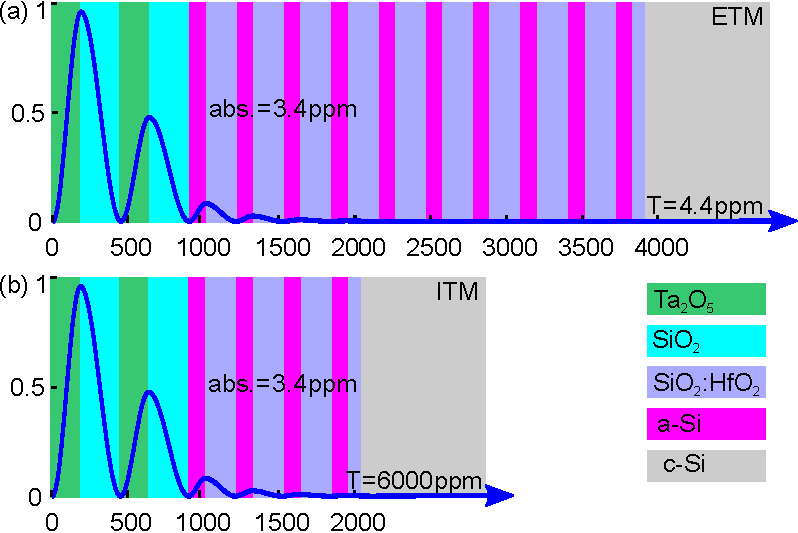
\includegraphics[width=12cm]{Detector/Optics/CoreOptics/Images/EFI_ETM_ITM_2.pdf}
	\caption{A multimaterial coatings design for (a) an ETM and (b) and ITM. This design uses an upper stack of SiO$_2$/Ta$_2$O$_5$ on top of a SiO$_2$:HfO$_2$/aSi lower stack~\cite{Craig_2019}. The blue lines show the electric field intensity as a function of depth in the coating.}
\label{fig:coatings:mulitmat}
\end{figure}

Several possible multi-material designs have been proposed to date~\cite{Steinlecher_2017,ion_plating,Pan_2018,Birney_2018,Craig_2019}\tcb{(comment MGranata:) there are 2 undefined references here}, including one that theoretically just meets the ET-LF coating thermal noise target for an optical absorption of 3.4\,ppm~\cite{Craig_2019}. This coating design relies on a level of absorption in aSi films which has been observed~\cite{Birney_2018}\tcb{(comment MGranata:) undefined reference here}, but has not yet been demonstrated reproducibly or on the scale required for ET.

Experimental verification of the performance of prototype multimaterial coatings has been reported~\cite{Gras_GWADW,Kinley_Hanlon_Warsaw} -- although it should be noted that a coating meeting the thermal noise and optical requirements of ET-LF has not been tested to date.

\paragraph{nanolayer coatings} -- Annealing at high temperatures is desirable to reduce the mechanical loss and optical absorption of many coatings: however, the onset of crystallisation (which results in higher mechanical loss and increased optical scattering) can limit the annealing temperature which can be used\tcb{(comment MGranata:) consider replacing "used" by "reached"}. The nanolayer approach involves making a single coating layer out of an array of thinner layers of two materials~\cite{Pan2014,Sankur1989}. This substructure can act to constrain crystallisation in the material, allowing higher annealing temperatures and lower mechanical loss to be achieved. This has been demonstrated for a high-index coating layer formed from a substructure of titania/silica nanolayers~\cite{Pan2014}.

More recently, it has been shown that the cryogenic loss peaks observed in silica coatings can be eliminated by using silica nanolayers separated with titania 'blocking' layers~\cite{Kuo2019}. Nanolayer coatings may therefore provide an excellent way to gain better performance from amorphous oxide materials at low temperatures. An important consideration for nanolayer coatings is to define the precision and uniformity with which each nanolayer needs to be deposited.\tcb{(comment MGranata:) I suggest adding here the following sentence: "To date, the deposition
of a full high-reflectivity coating embedding composite nanolayers has yet to be
achieved."}

\paragraph{Coating structure and mechanical loss} -- Significant progress has been made in predicting the cryogenic mechanical loss of coating materials computationally using molecular dynamics simulations~\cite{Hamadan2014,Trinastic2016,Billman2017}\tcb{(comment MGranata:) Please, add here also the following reference: F. Puosi et al., Phys. Rev. Res. 1, 033121 (2019).} and to obtain agreement with trends and magnitudes of experimental loss data.

Other structural work has shown the room-temperature loss may be correlated with medium-range order in Ta$_2$O$_5$ coatings, with more ordered structures and lower loss resulting from heat-treatment~\cite{Hart2016}. The evidence points towards the possibility that the same structural features responsible for low loss at room-temperature may be responsible for higher loss at cryogenic temperature. Raman spectroscopy studies have identified correlations between the ring structures and loss in silica coatings~\cite{granata2018correlated}. \tcb{(comment MGranata:) Please, add here also the following sentence and reference: "Very recent work has shown that a correlation exists between optical properties and internal friction in high-index oxide coatings [x]." 
[x] Amato et al., Sci Rep 10, 1670 (2020).}

Recently, evidence that specific structural units may correlate with lower loss has been found, in particular glassy structures with a high degree of corner-sharing, rather than edge or face sharing, between neighbouring tetrahedrons~\cite{Parsai2019}. This allows the structures of potential coating materials - many of which are well characterised - to be examined, and promising materials exhibiting a high degree of corner sharing to be identified and further investigated.

This increased understanding of the links between atomic structure and coating loss is a highly useful tool for developing lower-loss coatings.

\subsubsection{Possible coating materials}

\paragraph{Amorphous silicon} --  Amorphous silicon has low mechanical loss at cryogenic temperatures~\cite{Liu_1997,Murray2015}\tcb{(comment MGranata:) undefined reference here}, and has a relatively high refractive index, allowing thinner coatings -- with correspondingly lower thermal noise -- to be made. Mechanical loss as low as 2$\times10^{-5}$ has been observed in aSi coatings at room temperature and at cryogenic temperatures, and even lower loss is possible for coatings deposited at elevated temperature~\cite{Liu2014}. Elevated temperature deposition allows the aSi to form an `ideal glass' structure -- a low entropy amorphous state with very low loss.

While aSi is a very attractive material for thermal noise reasons, the optical absorption has historically been too high for use in gravitational wave detectors. Commercially grown ion-beam sputtered aSi coatings can have optical absorption of 1000 to 10000\,ppm at 1550\,nm (for a room-temperature HR stack made of aSi and SiO$_2$)~\cite{Steinlechner2016,Birney2018}. Significantly lower absorption can be achieved using a commercially available ion plating technique~\cite{ionplating}, and even lower again via electron cyclotron resonance (ECR) ion-beam sputtering~\cite{Birney2018}. The absorption of aSi tends to be significantly lower -- between a factor of 5 and 10 -- at $\sim$2000\,nm than at 1550\,nm~\cite{ionplating}. Operating ET-LF at a wavelength close to 2000\,nm may therefore be desirable to enable the use of aSi coatings for thermal noise reduction. While the absorption of the best aSi measured is still too high to allow a traditional aSi-based coating to be used, the incorporation of aSi layers into a mutimaterial coating design can allow significant thermal noise improvements while minimising the absorption contribution of the aSi layers.

aSi may also be a candidate material for a room-temperature coating. However, without further reductions in optical absorption, this is significantly more likely for a laser wavelength of 1550\,nm than for 1064\,nm, due to the higher optical absorption of aSi at 1064\,nm. However, it is interesting to note that some thermal noise reductions may be possible using aSi in a multi-material design at 1064 nm.

\paragraph{Silica coatings} \tcb{(comment MGranata:) I suggest changing the name of this paragraph to "Fluorides" and adding some text at the end of it, see below. Another option could be "Alternative cryogenic low-index layers"}-- For room-temperature detectors, efforts have largely focussed on improving or replacing the high-index coating layers which currently dominate the thermal noise. The current low-index material, silica, has a relatively low loss (as low as 4.5$\times10^{-5}$) at room temperature\tcb{(comment MGranata:) a most recent analysis shows that it is rather $\sim$2 $\times10^{-5}$: M Granata et al., https://doi.org/10.1088/1361-6382/ab77e9}. However, the loss of silica films increases significantly at cryogenic temperatures~\cite{Martin2014} - with both the structure and the magnitude of the loss being strongly dependent on post-deposition heat-treatment temperature~\cite{RobieThesis}. Therefore alternative low-index materials to silica will be required at for cryogenic coatings. A lower-loss low-index material is also likely to be required to achieve the required reduction in coating thermal noise at room temperature, although at the moment thermal noise remains dominated by the high index Ta$_2$O$_5$ layers. The room-temperature loss of silica can be further reduced by annealing at higher temperatures up to 900$^\circ$C\tcb{(comment MGranata:) please add here the reference supporting this statement: A. Amato et al., J.  Phys.: Conf. Series 957, 012006 (2018).}. In current coatings, crystallisation of the tantala layers prevents annealing above $\approx 600^\circ$C\tcb{(comment MGranata:) please add here the reference supporting this statement: A. Amato et al., J.  Phys.: Conf. Series 957, 012006 (2018).}.

\tcb{(comment MGranata:) I suggest adding the following text here: "In order to replace SiO$_2$ layers with lower-index materials, the optical properties and the internal friction of sputtered MgF$_2$ and AlF$_3$ coatings have been characterized at room temperature [Granata20]. Lower refractive index, higher optical abosrption and internal friction have been observed. Work is ongoing to characterize the impact of annealing on absorption and internal friction, at room and low temperature, for possible implementation in future cryogenic detectors like ET-LF."
[Granata20] M. Granata et al., Appl. Opt. 59, A229 (2020).}.

\paragraph{Silicon nitride} -- Silicon nitride films can have mechanical loss in the order of $1\times10^{-5}$ around 10\,K~\cite{Liu_2007} for a film on a substrate, and less than $1\times10^{-6}$ for substrate-free films~\cite{Southworth2009}. The refractive index of SiN is relatively low, making it of interest as a low-index material for use alongside aSi~\cite{Pan2017,ionplating}. Studies have shown that the exact composition of SiN films can strongly affect the refractive index, optical absorption and mechanical loss. Large enough refractive index variations can be obtained by changing the composition to potentially allow SiN to be used for both the high and low index coating layers. The optical absorption of SiN can be similar to the best aSi commercially available aSi films~\cite{Pan2017,Steinlechner2017}. A multimaterial design has been proposed to further reduce this absorption to below 5\,ppm for an HR stack ~\cite{Pan_2018}, although this design does not meet the ET-LF thermal noise requirements. 

Low mechanical loss has also been demonstrated in silicon nitride at room temperature and in sputtered films~\cite{Amato_2018}\tcb{(comment MGranata:) please replace this reference with a most recent one with updated data: M. Granata et al., Appl. Opt. 59, A229 (2020).}. Silicon nitride can withstand annealing at higher temperatures than tantala, \tcb{(comment MGranata:) please add here: "up to 900 $^{\circ}$C [x],"
[x] M. Granata et al., Appl. Opt. 59, A229 (2020).} allowing for the possibility of high-temperature annealing to produce a low loss Si$_3$N$_4$/SiO$_2$ coating.

\paragraph{Silica-doped hafnia} -- HfO$_2$ coatings have been shown to have lower cryogenic mechanical loss than SiO$_2$ and Ta$_2$O$_5$, but the material partially crystallises on annealing, resulting in poor optical properties~\cite{Abernathy_2011}. Doping HfO$_2$ with SiO$_2$ prevents crystallisation due to annealing, without increasing the cryogenic loss. With reasonably low optical absorption, SiO$_2$-doped HfO$_2$ shows promise for use as a low-index coating material to use with \tcb{(comment MGranata:) consider replacing "to use with" by "together with".}high-index aSi layers at cryogenic temperatures~\cite{Craig_2019}. This material is not of interest for ET-HF due to a relatively high room-temperature loss~\cite{CraigThesis}.

\paragraph{Alumina} Al$_2$O$_3$ coatings can have a lower mechanical loss than SiO$_2$ at cryogenic temperatures~\cite{RobieThesis}. While the refractive index is not as low as for SiO$_2$, this material may be of interest for use as a low-index material alongside materials like aSi which has a particularly high index. There has been interesting evidence that alumina coatings deposited at elevated temperatures can have significantly lower cryogenic loss than coatings which are heat-treated after deposition (REFERENCE - Abernathy?)\tcb{(comment MGranata:) I agree that a reference to the work of Abernathy et al. would be appropriate here, though -to my knowledge- only restricted-access LVC presentations are available to date?}.

\paragraph{Other amorphous coatings}
Improved amorphous oxides, with improvements being targeted using improved knowledge of the links between loss and structure, remain of interest for room-temperature coatings in particular. Options under investigation \tcb{(comment MGranata:) I can suggest a review article to be possibly cited here, covering all these options: M. Granata et al., Appl. Opt. 59, A229 (2020).}include studies of doping/mixing to increase crystallisation temperature and enable high-temperature annealing, the formation of ideal glass states using elevated temperature deposition and identifying materials with a high degree of corner-shared structural units. 

\paragraph{Crystalline coatings}

Multilayer single-crystalline coating materials can be grown epitaxially and can have very low mechanical loss. GaAs/AlGaAs crystalline coatings have been studied extensively, with a loss of 5.4$\times10^{-6}$ demonstrated at 20\,K for substrate-free resonator~\cite{Cole_2012}. Room temperature thermal noise measurements in small cavities are consistent with a coating loss of 4$\times10^{-5}$ at room temperature, and excellent optical absorption and scattering have been observed at wavelengths around 1550\,nm and 2000\,nm~\cite{Cole_2016}. AlGaAs coatings are grown on GaAs substrates, and would require to be transferred and bonded to a silica or silicon mirror - a process that is well-developed, at least for relatively small mirrors\tcb{(comment MGranata:) I do not agree with this sentence, since {Penn2019} has shown that there are relevant bonding issues even with 3" samples. I suggest replacing by "a process that might need further development"}. Currently the maximum available diameter of GaAs wafers is 20\,cm, which is not large enough for ET mirrors. However, there is now industrial interest in the production of larger GaAs wafers, with progress towards wafer diameters up to 30\,cm.\tcb{(comment MGranata:) I suggest that at some point in this paragraph above, the risk of many defects (up to 50 microns), showed again by {Penn2019}, should be also mentioned.}

Recent work suggested that the bulk loss of AlGaAs may be significantly higher than the shear loss~\cite{Penn2019}. Since the total coating thermal noise is more sensitive to bulk than to shear loss, this requires more investigation. It should be noted that low thermal noise has been directly measured in AlGaAs coatings, although so far only on relatively small mirrors with small laser beams~\cite{Cole_2013}.

GaP/AlGaP crystalline coatings have also been investigated~\cite{Lin}, with mechanical loss as low as 2.5$\times10^{-5}$ measured at 20\,K~\cite{Cumming_2015}. This material is of interest as it is lattice-matched to silicon and can be grown directly onto silicon substrates, potentially removing the need for substrate transfer (although growing a coating on an ET-sized mirror is unlikely to be feasible). Measurements of an initial highly-reflective stack showed high optical absorption of 2.3$\%$~\cite{Lin_2015}: however, there may well be scope to reduce this absorption e.g. be reducing impurities in the coating materials and coating chambers.\tcb{(comment MGranata:) I suggest to add also the following: "Also, to
date, the number of layer in a high-reflectivity coating is limited [x], resulting in a limited reflectivity."
[x] Cumming et al., Class. Quantum Grav. 32, 035002 (2015).}

For both GaAs/AlGaAs and GaP/AlGaAs coatings, the difference in refractive index between the two materials is relatively small, and so many layers are required to provide high reflectivity, reducing some of the thermal noise improvements due to the low loss.

\paragraph{Coating deposition}
The ET mirrors will be significantly larger than current gravitational detector mirrors, and ensuring the required coating uniformity over larger diameters will require development of coating deposition facilities. This development is already underway at the state-of-the-art coating facility at LMA. Problems with point absorbers and with bubbles - possibly of the sputtering ions used to deposit the coating - have been observed in the coatings for Advanced LIGO and Advanced Virgo: work to understand the origin of these defects and to eliminate them is a priority. \tcb{(comment MGranata:) I suggest to remove "and with bubbles" from the sentence above and to add the following sentence at the end of this paragraph: "Also, the occurrence of bubble-like defects limiting the annealing temperature of different coatings (high-index oxides) has been observed in multi-layer high-reflective stacks, work is currently ongoing also to understand and solve this issue".}

\paragraph{Strategy for ET}

Significant progress has been made towards development of coatings suitable for use at low temperatures in ET-LF. There are several highly-promising routes to meeting the coating thermal noise and optical absorption requirements. However, further study is required of the potential trade-off between coating absorption requirements, suspension thermal noise, ultimate mirror temperature and substrate thermoelastic noise -- and it seems likely that lower absorption than 5\,ppm may be required.

Achieving significant reductions in coating thermal noise at room temperature may be more challenging than at low temperature. Work in this area is ongoing, both for ET and for upgrades to the aLIGO and Advanced Virgo detectors, and there are several promising avenues\tcb{(comment MGranata:) consider replacing "avenues" by "options"}. One limitation is that some coatings which show promise for the low-temperature detector at 1550\,nm have significantly higher optical absorption at 1064\,nm, the wavelength envisaged for the room-temperature detector. Detailed studies of the benefits of operating the room-temperature detector at 1550\,nm may be of interest, as this may allow significant thermal noise reductions through the use of e.g. aSi-based coatings.

%A thin coating (few micrometers thick) is added to the polished substrates to create the optical function. For the arm cavities, the coating is a very high reflective reflector made of layers of alternate materials to form a Bragg grating. The constraints on the coating are extremely stringent as the coating must induce minimal displacement noise as well as very low optical loss.

%More specifically the coating Brownian thermal noise is the dominant source of noise and is expected to limit the sensitivity of Advanced detectors. So to further increase the detection range, intense worldwide research is currently lead to find better materials for the coating \cite{granata2019progress}. The Einstein Telescope will fully benefit from this research. 

%It is worth noting that compared to current interferometers, the impact of thermal noise on the ET noise budget is mitigated thanks to longer arm length and larger beam size.

%\paragraph{Room temperature interferometer}

%ET-HF share the same coating specifications as the Advanced LIGO + upgrade, to be operated around 2022 (a coating loss angle reduced by a factor 3 compared to current mirrors). So far no coating formulas or recipe have been found to match this requirement on large size, however people are optimistic that at the time of ET such coating would be present and well tested.


%\paragraph{Cryogenic interferometer}

%The cryogenic interferometer benefits from the lower temperature as the displacement induced by thermal noise scales as the square root of the temperature. A recent design using a multi-material approach (with the usual Ta$_2$O$_5$ and SiO$_2$ layers on top of a stack SiO$_2$:HfO$_2$ and amorphous silicon layers) has shown to meet the requirement for ET-LF \cite{craig2019mirror} for both the coating thermal noise and the optical absorption. 


\paragraph{Other core optics}

Central interferometer optics such as Power and Signal Recycling Mirrors (PRM and SRM) or beamsplitter will be smaller in size (diameter in the order of 10~cm) and at room temperature. Fused silica is hence the preferred material for the substrates. The coating will use the same materials as for ET-HF to benefit from state of the art deposition process. The procurement of those optics does not represent any challenges and will be straightforward.

\subsection{Light sources}
% Author: Benno Willke
\label{Sec:Lasers}
\label{sec:lasers}

%\tcb{version 5 Nov 2019 B. Willke}

Each of the ET interferometers will use a high power laser system with low
intrinsic noise called the high power laser (HPL) in the following. As no
current laser design can meet the ET stability requirements several nested
stabilization control loops are required to  reduce the fluctuations of the
free-running laser before the light can be injected into the main
interferometer. Like in all currently operating GWDs a first ET laser
stabilization layer will be installed on a seismically isolated laser table
outside the vacuum system. The combined system of HPL and this stabilization
layer is called the prestabilized laser (PSL) and is discussed in this section.
We will start with a discussion of the PSL requirements for ET-LF and ET-HF
followed by a description of the HPLs for both interferometers. The last
subsection will discuss passive and active noise reduction concepts that will
prepare the light for injection into the suspended input modecleaner (IMC).
%described in the \tcb{auxilliary optics subsection} %\ref{sec:{Auxilliary
%Optics}}.

{\bf Requirements}\\
The ET-HF HPL has to operate in a single-frequency continuous-wave (cw) mode at
a wavelength of 1064\,nm and needs to deliver 700\,W in a linear polarized
fundamental spatial $\rm HG_{00}$ mode. With the assumption of roughly 30\% loss
between the laser and the IMC output this leaves 500\,W at the input of the main
interferometer. The higher order mode content of this laser should be below 10\%
and the polarization purity at least 1/10. The ET-LF HPL needs to operate in a
single-frequency continuous-wave (cw) mode at a wavelength of approximately
1550\,nm with similar spatial and polarization purities as the ET-HP HPL. A
laser power of 5\,W is required to allow for 3\,W to be injected into the main
interferometer. 

Both HPLs need to provide actuators with sufficient dynamic range and speed to
allow for a suppression of their free running laser frequency-, power- and
pointing noise and to compensate for noise introduced between the PSL interface
on the laser table and the main interferometer's reference frame. The relative
power noise (RPN) in the megahertz frequency range should be shot noise limited
for 100\,mA photo current. In addition the HPLs need to operate reliable  with
small drifts and only limited maintenance requirements. 

Without a detailed interferometer design only a rough estimation of the ET PSL
noise requirements can be given. The frequency noise of the light injected into
the IMC will be subject to Doppler noise between the laser table and the
suspended reference frame. A frequency noise in the $10\,\rm{mHz} /
\sqrt{\rm{Hz}}$ range should be well below this level and hence adequate as PSL
requirement. Following the same line of thought the beam pointing requirement of
the ET PSLs will be similar to the one of advanced GWDs with relative lateral
and angular beam fluctuations in the $10^{-6} / \sqrt{\rm{Hz}}$
range\cite{Kwee2012}. With a similar power noise coupling and a 10 fold improved
sensitivity compared to the advanced GWDs the ET detectors would need a factor
of ten better laser power stability of roughly $\rm{RPN} = 3\!\times\!10^{-10} /
\sqrt{\rm{Hz}}$. 


{\bf High power laser}\\
 It is likely that the 700\,W laser power for ET-HF will be generated by a
 coherent combination of several high-power laser-amplifier stages seeded by one
 or more low-power low-noise master laser(s). Two different concepts are
 currently under investigation for such master-oscillator power-amplifier (MOPA)
 stages at the 250\,W output power level. One concept is based on
 mode-selectively pumped Nd:Vandat amplifiers which do not suffer from
 depolarizaton problems as Nd:YAG systems would do. A power of roughly 200\,W
 was lately generated with a commercial neoVAN-4S-HP amplifier chain with low
 noise and high spatial purity \cite{Bode2020, Willke2019}. Investigations are
 underway to increase the output power of such a solid state amplifier chain to
 250-300\,W. As solid-state MOPA chains are more complex compared to fiber based
 MOPAs, solid-state MOPAs serve as fall back solutions for ET-HF HPLs and will
 not be further discussed in this document.
 
Fiber amplifiers offer a highly-efficient and compact way to amplify laser light to the kW level. The amplification of narrow linewidth single mode seed lasers is, however, limited by nonlinear effects such as stimulated Brillouin scattering (SBS). Large mode-area (LMA) fibers in combination with losses for high-order spatial modes introduced by bending of the fiber can lead to high SBS free output powers in a single spatial mode operation. Sophisticated fiber designs (photonic crystal fibers \cite{Limpert2006}, photonic band gap fibers \cite{Gu2014} and chirally-coupled-core fibers \cite{Ma2014}) can guide a single mode with a large mode field diameter even without such bending losses.
The SBS threshold can be further increased by a differential temperature induced shift of the SBS gain spectrum along the fiber and via a counter-propagating pumping scheme. Several high power fiber amplifier systems that meet the demanding ET-HF HPL noise requirements have been demonstrated up to power levels of 300\,W \cite{Theeg2012, Zhao2018, Wellmann2019} .
%A 300\,W fiber amplifier system that meets the high spatial purity and low noise requirements was demonstrated by Theeg et al. \cite{Theeg2012, Wellmann2019} and a low noise 100\,W fiber amplifier system was reported by Zhao et al. (\cite{Zhao2018}). 
Higher power levels generated with fiber based MOPAs were reported in literature but only limited information on spatial purity and noise performance of these systems is available. Especially informaiton on the relative power noise (RPN) at radio frequencies is missing which is prone to increase at pump power levels well below the onset of significant SBS related power in the back-ward propagation direction \cite{Zhang2005}. Hence a conservative approach is taken for ET-HF that assumes that several fiber based MOPA systems will be coherently combined to form the ET-HF HPL. 
These fiber amplifier modules will each incorporate a mode-field adapter, a pump-light stripper, an active fiber and a pump-light combiner that couples the light of the fiber based pump diodes into the active LMA fiber. The amplified light will leave the fiber via a fused silica end cap to reduce the light intensity at the glas air interface and with this the risk of contamination induced damage.

Different options are under investigation for the seed laser design. A
fiber-oscillator in combination with a fiber-preamplifier allows for an
monolithic all fiber design that includes fiber based components such as Faraday
isolators (FIs), electro-optical modulators (EOMs) and acousto-optical
modulators (AOMs). All these components including the high power LMA amplifier
are spliced together and form a monolithic HPL module. One disadvantage of this
concept is, that modulators can only be used between the seed and the
preamplifier due to limited power handling capabilities of fiber modulators.

A second concepts relies on the non-planar ring-oscillator (NPRO) seed as used
in all currently operating GWDs. Free space EOMs, AOMs and FIs can be used to
condition the laser light before it is coupled into either a solid-state or a
fiber pre-amplifier. This amplifer is either spliced or free space coupled to
the mode-field adapter of the LMA high power amplifier. A trade-off study
between these two concepts will lead to the final ET-HF seed laser concept. Both
seed laser concepts can provide  actuators with enough range and speed for the
PSL frequency stabilization. As the power noise of a MOPA system is usually
dominated by the high power amplifier and as the modulation of the pump diodes
of this stage offer a large actuation range without cross coupling to the laser
frequency, the pump current of the LMA amplifier's pump diodes will serve as the
main PSL power actuator.

The coherent combination will be performed on a beam combiner (beam splitter)
before the pre-modecleaner cavity (PMC, see next subsection) . Both of the to-be
combined beams are separately aligned to the Eigenmode of the PMC which
guarantees an optimal spatial overlap. The differential phase between the beams
will be sensed at the second beam combiner port. A phase-lock control loop will
feed back to either one of the seed lasers (in case different seed lasers are
used) or to a piezo-controlled mirror or a fiber strecher in one amplifer's beam
path (in case of a single seed laser). Long term test will reveal if alignment
control loops are required to keep a good interference contrast at the beam
combiner.

Several commercial seed laser operating at 1550\,nm and Erbium based fiber
amplifiers for the same wavelength are available for use in ET-LF. The seed
lasers are either based on fiber oscillators or external-cavity diode lasers to
generate low noise beams with several 10\,mW power. Several MOPA configurations
with Er fiber amplifiers were tested at the 2\,W level and show spatial purity
and noise levels consistent with ET-LF requirements \cite{Meylahn2019}. The
amplification to the required power level of 5\,W by a second Er fiber amplifier
is straight forward. (Low noise fiber amplifiers with output power of more than
100\,W have been demonstrated \cite{deVarona2017}). In the case of a laser diode
based seed laser the pump current can be uses as a fast frequency actuator with
50\,kHz actuation bandwidth. The power noise can be reduced by feed-back to
either the fiber amplifier's pump diodes or via an external electro-optical
amplitude modulator (EOAM).

{\bf Prestabilization}\\
Even though laser systems with very low free running power and frequency noise
are chosen for ET sophisticated nested stabilization schemes are required to
achieve stability levels in the interferometers that do not limit the GW
sensitivity. A first stabilization layer, the so called prestabilization is
performed on the laser table outside the vacuum system. The goal of the
prestabilization system is to reduce the laser fluctuations well below the level
of noise added by the Doppler and beam pointing effects due to motion of the
laser table with respect to the seismically isolated interferometer frame.
Power in higher order spatial modes as well as beam pointing fluctuations are
reduced by passive spatial filtering with stable optical ring resonators called
modecleaner (PMC in case of the filtering on the laser table).  In the case of
ET-LF a fiber could be used as a spatial mode filter and as a tranfer fiber to
deliver the laser light via a seismically isolated output coupler in the
interferometer reference frame. This could strongly reduce the noise introduced
between the laser table and the suspended modecleaners. Further investigations
will reveal if non-linear effects or added phase noise in such a fiber would
prevail the benefits. In the case of ET-HF the power levels are to high for a
fiber based modecleaner such that a PMC needs to be part of the PSL. A PMC has
the additional benefit, that it filters power noise at rf frequencies and that
it can provide spatially stable pick-off ports for the frequency and power
stabilization and potentially for phase look loops of the squeezing or length
and alignment control subsystem.

The PSL frequency stabilization will use a rigid spacer high Finesse reference
cavity which is seismically isolated inside a vacuum system. A feedback control
loop with a high unity gain frequency of several hundred kHz is required to
allow for high bandwidth second layer control loops. These will use the
suspended modecleaner and the main interferometer as frequency references and
will feed back either via a summation point into the error point of the PSL loop
or to an AOM frequency shifter placed between the main laser and the rigid
reference cavity.

A high unity gain frequency is as well required for the PSL power stabilization
control loop. This needs to reduce the relative power noise (RPN) of the beam
leaving the PMC to roughly $10^{-8} / \sqrt{\rm{Hz}}$. As the speed of the
feedback to the diode laser pump source of the HPL is limited to several 10\,kHz
a fast EOAM after the seed laser or the pre-amplifier will be part of this
control loop. The power noise sensor for the power stabilization loop will be a
high-power photodiode placed into one of the pick-off ports of the PMC. Due to
pointing-to-RPN or polarization-to-RPN coupling by the suspended input
modecleaner a sensor for the second layer power stabilization has to be places
after the modecleaner close to the power recycling mirror. The second layer loop
power stabilization loop will either feed back into the error point of the first
loop or to an in-vacuum EOAM to achieve an RPN in the $10^{-10} / \sqrt{\rm{Hz}}$ range. Depending on the final RPN requirements sophisticated
power noise sensing schemes based on multi-photodiode arrays\cite{Kwee2009}, the
optical AC coupling technique \cite{Kaufer2019} or squeezed light assisted power
noise sensing \cite{Vahlbruch2018} might be required for this second loop. 

The general PSL layout will be very similar for the ET-HF and ET-LF PSLs. Due to
the two orders of magnitude lower power level the stabilization of the ET-LF
laser might be easier as more integrated fiber components can be used. These
have typically higher bandwidth and are less alignment sensitive. This small
advantage might, however, be compensated by the fact that the ET-LF requires
stability at much lower Fourier frequencies. This is generally harder as
scattered light and beam pointing coupling to the control loop's sensors is
larger at low frequencies. 

Prototypes for both the ET-HF and ET-LF PSLs will be set up in research labs in
the near future to test the ET laser designs, the stabilization concepts and to
gain insight into the longterm drift behavior of such systems.
 

\label{sec:Squeezers}

\subsection{Squeezed light sources}

\bluecomment{SS: should this section move to after the next one, i.e. after the discussion of quantum-noise reduction techniques?}

Squeezed states of light \cite{Yuen76,Walls1983,Breitenbach97} provide a way of increasing the sensitivity of a gravitational wave detector in the quantum noise limited region, independently of the circulating light power. Generally, a light field is described by two non-commuting physical quantities, the amplitude and phase quadratures. The minimum product of their uncertainties is limited by Heisenbergs uncertainty relation, which is also valid in the complete absence of photons, that is for a vacuum state. Vacuum states as well as coherent states have noise equally distributed in the field quadratures. Squeezed states show a noise below the vacuum noise level, however, owing to the Heisenberg uncertainty principle, this is not possible for all quadratures of the state simultaneously.  

For a Michelson interferometer operated close to a dark output port, squeezed states can be used by injecting them into the signal port and spatially overlapping them with the high power laser field at the beam splitter \cite{1981_PRD.23.1693_Caves}. The squeezed quadrature has to be controlled such that, after being reflected off the interferometer, it is in phase with the readout (amplitude) quadrature of the observatory output light. For reviews on the application of squeezed states of light in the framework of gravitational wave detectors we refer to Refs. \cite{Schnabel2010,Schnabel2017,Barsotti2018}.

Squeezing has a significant impact if large squeezing factors can be produced and detected. For example, an effective squeezing level of 3\,dB improves the signal-to-noise ratio by a factor of $\sqrt{2}$ at shot-noise limited frequencies, which is equivalent to doubling the interferometer's input laser power. An effective squeezing level of 10\,dB would correspond to a ten-fold power increase. Here, effective squeezing does not refer to the injected squeezing initially available, but rather describes the quantum noise reduction measurable with the photo detector(s) at the observatory's output.  
%
Any optical loss between squeezing generation and detection reduces the level of measurable squeezing. Therefore, a prerequisite for the 10\,dB of effective squeezing envisaged for ET, is a squeezed light source design that can provide sufficiently strong squeezed vacuum states of light at the expected gravitational wave signal frequencies ranging from 10 Hz to 10 kHz. 

Significant progress has been made over the last 10 years in the generation of squeezed vacuum states of light and squeeze factors beyond 10\,dB are routinely produced at the two required wavelengths, 1064 nm and 1550 nm, respectively.
%
In the same manner as today's most efficient squeezed light sources, the ET-squeezers will employ cavity-enhanced parametric down-conversion, also called optical parametric amplification, where the interaction between the fundamental and second harmonic fields via a $\chi^{(2)}$-process inside a non-linear crystal produces non-classical photon-pair correlations that yield a reduced noise variance in a certain field quadrature.  
%
%Cavity enhanced squeezed light generation can be realized with different optical topologies.  
%
%
\begin{figure} %[htbp]
\centering
{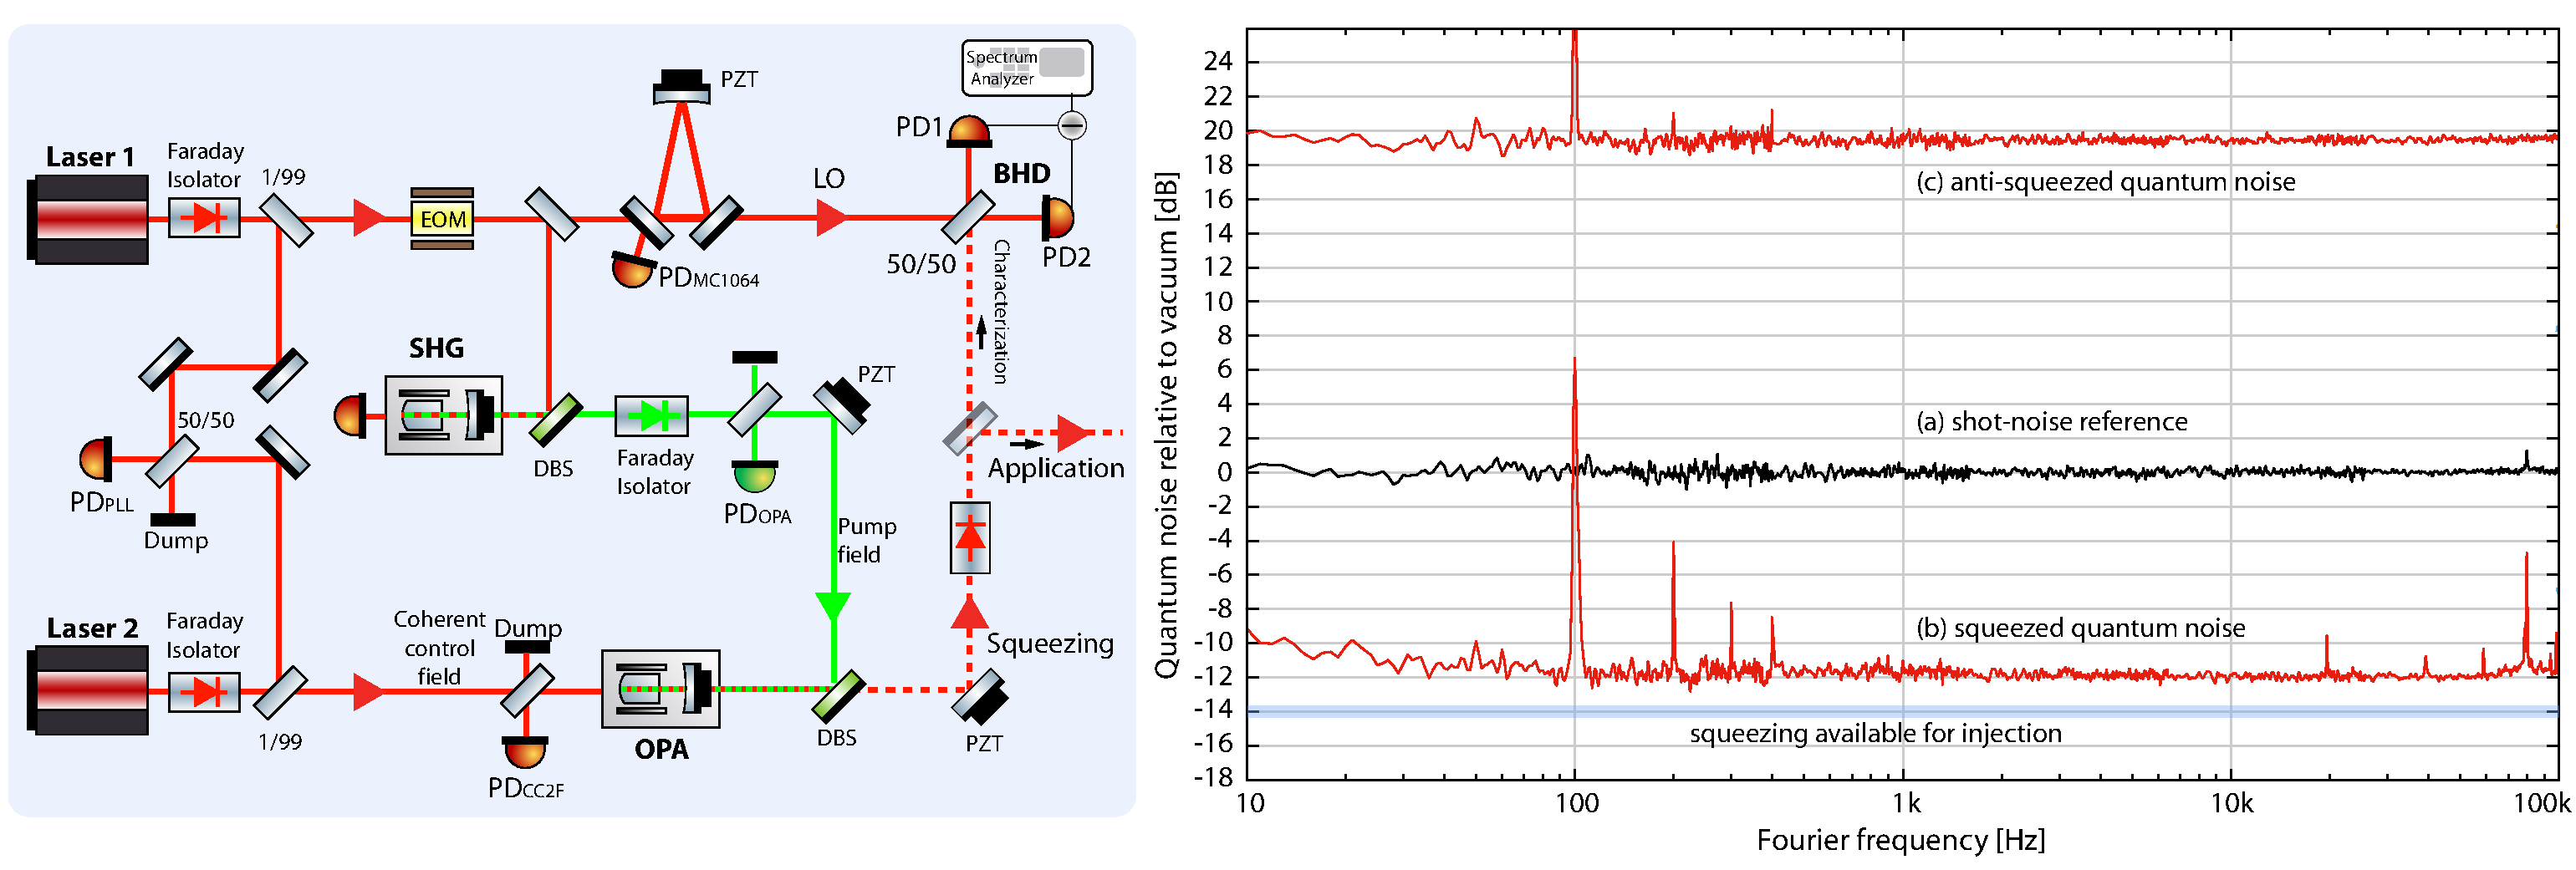
\includegraphics[width=\linewidth]{Detector/DetFigures/SqueezerFig1b.pdf}}
\caption{{\bf{Left:}} Schematic for the generation and coherent control of squeezed vacuum states of light. Laser 1 provides the light field for homodyne detection and for frequency doubling in a second harmonic generator (SHG). The SHG provides the pump field required for the generation of squeezed vacuum states in an optical parametric amplifier (OPA) operated below threshold. The squeezed vacuum states are extracted via a dichroic beam splitter (DBS) and send towards the interferometer. Alternatively, the squeezing level can be characterized by means of a balanced homodyne detector (BHD).  A Faraday isolator is implemented in the squeezing path to protect the OPA from light scattered back from the interferometer.\\
{\bf{Right}}: Quantum noise squeezing as reported in \cite{Mehmet2018}. Trace (a) represents the shot noise reference (normalized to 0\,dB) measured with a homodyne detector. In reference to this trace the measured quantum noise powers for squeezing (b) and the corresponding anti-squeezing (c) are shown.
Up to 12\,dB squeezing and 19.6\,dB anti-squeezing was observed, which is consistent with a theoretical model assuming a residual phase noise of 3.5\,mrad rms and an overall optical loss of 5.3\,\% for the squeezed field. This includes 2.5\,\%  optical loss due to the homodyne detection which needs to be subtracted to deduce the squeezing level available for the injection into a gravitational wave detector. This level is indicated by the blue area and corresponds to a squeezing factor of 14\,dB.}
\label{SqueezerFig1}
\end{figure}
%
The strongest squeezing level demonstrated to date is a squeeze factor of 15\,dB below the classical shot-noise limit at the wavelength of 1064\,nm, but only measured at MHz frequencies~\cite{Vahlbruch2016}. The topology of the optical parametric amplifier (OPA) used therein was a linear, standing-wave, doubly-resonant cavity with a non-linear crystal made from periodically poled potassium titanyl phosphate (PPKTP).  
%
Up to 13\,dB of non-classical noise suppression was measured at a wavelength of 1550\,nm~\cite{Schonbeck18} in a similar cavity design, but again only at MHz frequencies. 
%
By the implementation of a coherent control scheme \cite{Vahlbruch2006} and the mitigation of parasitic interferences the frequency band of detectable squeezing can be extended from MHz down to the required GW-frequencies \cite{Vahlbruch2007}. 
This has been demonstrated in tabletop experiments with various squeezed light source setups operated in-air or in-vacuum and with OPAs constructed as bow-tie or linear resonators \cite{Vahlbruch2006,Stefszky2012, Wade2016}.
%
Following these developments, similar schemes were used to realize squeezing enhancement in large scale gravitational wave detectors. 
The first successful implementation was achieved at the GEO600 detector in 2010 and since then squeezing has been routinely applied \cite{2011_Nat.Phys.7.962_LSC, Grote2013}. 
The Advanced Virgo and the two Advanced Ligo detectors have been also upgraded to include the squeezing technique since the O3 science run in early 2019.  
%

The most efficient \bluecomment{SS: what's efficient in this context, and/or is it relevant?} squeezed light source at GW-frequencies so far was reported in 2018 \cite{Mehmet2018} at AEI Hannover. Figure \ref{SqueezerFig1} summarizes the main result of this work, where squeezed light was generated in a linear, doubly-resonant OPA at a wavelength of 1064\,nm. A quantum noise reduction of up to 12\,dB at Fourier frequencies between 10\,Hz and 100\,kHz was directly measured with a diagnostic homodyne detector. The analysis revealed that the measured squeezing level corresponds to an equivalent squeezing factor of up to 14\,dB available for the injection into a gravitational wave detector with only 3.5\,mrad rms of phase noise attributed to the squeezed light source operated in air \bluecomment{SS: how does this compare to the assumed effective squeezing level of 10dB of Table3.1? Maybe link to Fig 3.7 to show that phase noise at that level should give sufficient margin.}. The recent progress in the development of low-loss Faraday isolators suggests that this squeezing factor can be even further improved in the near future \bluecomment{SS: reference? Is this also valid for 1550nm?}. 
At the wavelength of 1550\,nm there are also so far no indications why a comparably high squeezing level should not be observable \bluecomment{SS: double-negative makes this a bit hard to read} at GW-detection-frequencies once a coherent control scheme is implemented \cite{Mehmet2011} \bluecomment{SS: I'm not aware of any (citeable) progress in that direction, but it feels like there should be.}. 

\bluecomment{SS: with the 532nm pump light, degradation of optics/crystals over time seems to be an issue. Has there been progress on this or are concepts foreseen that might reduce downtime? Do we expect better long-term performance at 775nm?}
Based on the demonstrated technical readiness, a total of six independent squeezed light sources will be engineered for ET: Three systems will generate squeezing at 1550\,nm for the ET-LF detector and three systems operating at 1064\,nm will be used for the ET-HF detectors. 

\label{Sec:Squeezers}
% Author: Moritz Mehmet, Henning Vahlbruch

\subsection{Quantum noise reduction}

%\subsubsection{Quantum noise reduction techniques}


In a laser-interferometric gravitational-wave detector, there are different types of noise sources, which are usually categorized into quantum noise sources and classical noise sources (cf.\ Sec.~\ref{sec:optlayout}). In terms of the noise, the main difference in the sensitivity of the different topologies comes from the spectral distribution of the quantum noise, even though there could also arise differences in the susceptibility to the classical noise, due to the fact that there are e.g.\ a different number of mirrors or different shapes of cavities. Therefore, the choice of topology is mainly defined by the choice of quantum noise reduction techniques used.

\textbf{Quantum noise} in the interferometers originates from the fundamental quantum fluctuations of light amplitude and phase that follow the Heisenberg uncertainty relation. Quantum phase fluctuations can be viewed as a manifestation of Poissonian statistics of the photons emitted by an ideal laser and thus limit the measurement precision of any interferometric device. This uncertainty of photons arrival time at the photodiode known also as \textit{shot noise} scales down with the increase of the number of photons used for the measurement and thus is inversely proportional to the light power interacting with the test masses of the interferometer. Amplitude fluctuations of light lead to the fluctuations of radiation pressure on the mirrors, resulting in the random motion of the mirrors and of the arm length change that
mimics the gravitational wave signal. This second component of quantum noise is known as \textit{quantum radiation-pressure} or \textit{quantum back-action} noise. It
naturally scales up with light power and is most prominent at the low frequencies, where massive suspended mirrors have higher response to the driving force. The fact
that quantum shot noise and then quantum radiation-pressure noise have an inverse dependence on power and that the underlying fluctuations of phase and amplitude are uncorrelated, gives rise to a so called standard quantum limit (SQL)~\cite{Braginsky1968,Braginsky1999} on continuous high-precision interferometric measurements. 

However the SQL is not a fundamental limitation on the achievable sensitivity of the interferometer, but rather a convenient benchmark for comparing different quantum noise mitigating schemes proposed so far for advanced gravitational-wave interferometry (see \cite{2019_LivRevRel_Danilishin} and references therein). It is also a vivid example of the trade-off one has to make between high sensitivity at shot-noise-dominated high frequencies vs. the reduced back-action-noise at low frequencies (below 10 Hz) which cannot be simultaneously attained in a conventional displacement-sensitive interferometer. This obstacle can be overcome by using 2 conventional interferometers instead of one, using a so called \textit{xylophone} configuration~\cite{Hild2010a}. 

Based on the requirements on the quantum noise sources (and technical ones, cf. Sec.~\ref{sec:optlayout}), we have chosen a xylophone configuration ~\cite{Hild2010a} as an optimal design of ET (cf. Sec.~\ref{sec:xylophone}). Each detector in a xylophone configuration is split into two interferometers, one optimized for low frequencies, operating at low light power and the other optimized for high frequencies operating at high light power. A xylophone configuration resolves two major problems:
\begin{itemize}
\item The simultaneous usage of high circulating light power for increasing the high-frequency sensitivity and cryogenic mirrors for decreasing thermal noise. In a xylophone configuration the low-frequency interferometer utilizes relatively low optical power which does not pose a problem of heating the cryogenic mirrors, while the mirrors at room temperature in the high-frequency interferometer allow use of much higher light power.
\item Simultaneous decrease of photon shot noise and radiation pressure noise. The sensitivity of the radiation pressure noise-dominated low-frequency interferometer benefits from low light power, while the sensitivity of the shot noise-dominated high-frequency interferometer benefits from the high light power.
\end{itemize}



There is nevertheless a fundamental limit on sensitivity more stringent than the SQL \cite{Miao2017b,Miao2017,2019_LivRevRel_Danilishin}. It sets the ultimate limit on the precision attainable for a given configuration of the interferometer and goes by name \textit{energetic quantum limit} \cite{00p1BrGoKhTh} in GW interferometry or by name \textit{quantum Cram\'er-Rao bound}~\cite{Tsang2011} in quantum metrology. In the context of laser interferometric gravitational-wave detectors, it can be expressed in terms of a power spectral density (PSD) of interferometer noise in the units of GW strain $h$:
\begin{equation}\label{eq:FQL_new}
S^h_{\rm FQL}(\Omega)=\frac{\hbar^2c^2}{S_{PP}(\Omega)L^2} = 
\frac{4\hbar^2}{S_{\cal E E}(\Omega)}\,. 
\end{equation}
Here $S_{PP}$ is the single-sided PSD for the fluctuations of optical power $P$ inside the arms and $S_{\cal EE} = 4 S_{PP} L^2/c^2$ is the corresponding PSD of fluctuations of light energy stored in the arms. This means that large uncertainty of energy of intracavity photons is necessary to probe the spacetime precisely, which is a direct upshot of the energy-time uncertainty relation. 

Reaching this fundamental quantum limit in a given configuration is a non-trivial task that requires using quantum noise reduction techniques. They have different, and often very special, requirements on the optical topology. The quantum-noise reduction techniques can be divided into two main groups: (i) those that engineer quantum correlations between the components of quantum noise with the goal of {\bf quantum noise cancellation} or reduction, and (ii) those that instead aim at modifying the response of the interferometer to the GW so as to {\bf amplify the signal}.

The former methods encompass a vast body of schemes, of which the most mature one is the injection of squeezed vacuum into the readout port of the interferometer first proposed by Unruh \cite{PhysRevD.19.2888}. It has successfully improved the sensitivity of GEO600~\cite{GEOsqueezing} and Advanced LIGO~\cite{Aasi2013NatPhot} detectors and is now considered as an integral part of any future GW detector design. Yet the injection of squeezed vacuum alone cannot lead to the desired broadband suppression of quantum noise because of the frequency dependent quantum correlations between the phase and amplitude fluctuations of the intracavity light as a result of the interaction between light and the mechanical motion of the mirrors~\cite{KLMTV}. The solution is to use frequency dependent squeezing injection technique~\cite{KLMTV} that is discussed in greater detail in Sec.~\ref{subsec:SQZforGWD}.

Despite its success, squeezing injection does not allow the interferometer to saturate the FQL. This calls for more sophisticated and yet experimentally unexplored
quantum noise cancellation methods known as {\bf quantum non-demolition (QND)} techniques that are covered below. 

The second group of methods is based on the idea that the spectral distribution of the SQL itself is not a fixed constant, but depends on the test object dynamics, i.e.\ on the (mechanical) susceptibility of the test mass, which relates the test-mass motion to all forces acting on it. Therefore, the free-mass SQL can be beaten by using a more responsive object and thus increasing its signal displacement---the harmonic oscillator as an example has much stronger response to near-resonance forces and therefore a better sensitivity than the free-mass SQL around the resonance frequency. Therefore, the sensitivity gain is obtained not by delicate cancelation of the
quantum noise, but by a classical {\bf signal amplification}. 

%%%%%%%%%%%%%%%%%%%%%%%%%%%%%%%%%%%%%%%%%%%%%%%%%%%%%%%%%%%%%%%%

\subsubsection{Review of quantum non-demolition topology options}
\label{subsec:qndopt}

The second generation laser-interferometric gravitational-wave detectors, Advanced LIGO detector~\cite{TheLIGOScientific:2014jea} and Advanced VIRGO detector~\cite{TheVirgo:2014hva}, are already limited by quantum noise in a major part of their detection band. Science objectives of ET (see Ch.~\ref{chap:ScienceCase}) and other next generation instruments instruments make it an imperative to improve low and high-frequency sensitivity by at least an order of magnitude as compared to the current machines. This cannot be done without using the QND techniques to suppress quantum noise below the SQL.

The impressive progress in mitigation of the technical noise sources in the current interferometers as well as an extensive current R\&D on reduction of thermal noise of the core optics (cf. Sec~\ref{Sec:CoreOptics}), on advanced seismic isolation (cf. Sec~\ref{Sec:SASandSUS}) and on Newtonian noise mitigation (cf. Sec~\ref{sec:mitigateNN}) allows to project that quantum noise will be the main obstacle towards reaching the design sensitivity of ET and  for further progress of GW interferometry in general. As there are natural limitations on the mass of the mirrors and on the achievable level of light power in the arms, the significant modification of interferometer topology, optical readout and use of non-classical light sources becomes an essential for the next generation GW detectors.

As we have seen in Sec.~\ref{sec:lshape}, there are different topology options available which can all be fitted into an L-shaped geometry. A plethora of various schemes that promise significant improvement in terms of quantum noise has been developed so far, which however require significant and sometimes drastic changes to 
the conventional Fabry-Perot--Michelson optical scheme. Many of them have great potential in reducing the quantum noise, but there is a big discrepancy in terms of readiness: some are far away from being ready to be implemented into gravitational-wave detectors, others have been already demonstrated experimentally as a proof of principle or have been even already implemented into gravitational-wave detectors. 
The non-exhaustive list of QND options in the descending order of experimental readiness/level of R\&D completeness 
 is presented below (more detailed description can be found in \cite{2019_LivRevRel_Danilishin}):
 \begin{enumerate}
 \item
 \textbf{Injection of (frequency-dependent) squeezed vacuum} in the readout port of the interferometer (see more detail in Sec.~\ref{subsec:QNRsqz})
uses inherent quantum correlations in non-classical states of light to reduce quantum fluctuations in the readout quadrature of the interferometer 
in the shot-noise-dominated frequency range \cite{1981_PRD.23.1693_Caves,2011_Nat.Phys.7.962_LSC,Aasi2013NatPhot,Schnabel2017}. 
Additional filter cavities can be used to rotate squeezing angle in an optimal frequency dependent way \cite{KLMTV,2013_OE.21.30114_Loss_in_FC_Isogai,Oelker2016}
to gain a broadband suppression of quantum noise. 
\item
\textbf{Conditional frequency-dependent squeezing} \cite{Ma_NPhys_13_776_2017} is a recent proposal that allows to achieve frequency dependent 
squeezing enhancement without filter cavities. It uses a nondegenerate two-mode squeezer that produces entangled beams with far detuned from 
each other frequencies, of which one, \textit{signal}, coincides with the pump laser frequency and another, \textit{idler}, is shifted by several MHz, and thereby passes through 
the interferometer gaining only optimal frequency-dependent phase shift. Detection of the idler beam projects the signal one into an optimal frequency dependent 
squeezed state that gives the desired sensitivity improvement. Recent table-top experiments at ANU \cite{2019arXivEPRsqzANU} and Hamburg \cite{2019arXivEPRsqzHamburg}
proved the viability of this technique, yet confirmed the penalty of twice the decoherence caused by the injection loss and the loss at the readout as compared to a single-mode 
squeezing-based schemes.
\item
\textbf{QND speed-meter interferometers} \cite{00a1BrGoKhTh,02a2Kh,Purdue2001,Purdue2002,Chen2003,04a1Da} offer an alternative way to mitigate back-action noise in an intracavity way.
This is achieved by modifying the way light passes through the interferometer so as to let it interact with the mechanical motion of the test masses two times sequentially in a coherent way, 
thereby making the readout signal proportional to the velocity of the mirrors and at the same time coherently subtracting a major fraction of back-action. Speed meters can be realised in many 
various ways, either using ring arm cavities\cite{Chen2003,2014_CQG.31.215009_Graef}, polarisation optics \cite{Danilishin2004,PhysRevD.87.096008,PhysRevD.86.062001,2018_PCSM_danilishin,2017_Phys.Lett.A_EPR_SM}, or simply adding a long-base ``sloshing'' cavity to a Michelson interferometer \cite{Purdue2001,Purdue2002,2019arXiv190904185F}. Apart from Michelson interferometers,
speed meters are arguably the most extensively studied and well understood interferometer topology, where the impact of real-world imperfections and asymmetries is analysed in great detail \cite{2015_NJP17.043031_asymSag, 2018_NJP.20.10.103040_QN_cancellation,2017_PhysRevD.95.062001}. 
\item
\textbf{Hybrid schemes} that seek to enhance sensitivity by coupling the interferometer light mode to a generally nonlinear quantum system.  
The first use of this approach was to create a so called \textbf{white-light cavity (WLC)}  \cite{Wicht1997} by introducing atomic gain medium in the arms
prepared in such a way to render negative dispersion for the signal sidebands. This would cancel the positive dispersion of the arm cavities 
and would result in a broadening of the bandwidth of the interferometer without sacrificing its peak sensitivity. The atomic medium,
however, has proven to be too noisy for the purpose of GW detection, but the two new promising approaches were suggested. The first suggests to place a 
nonlinear (squeezer) crystal in the signal-recycling cavity \cite{Korobko2017} and the other suggests to use an unstable optomechanical filter instead \cite{Miao2015a,Peano2015}. 
The main advantage of the WLC-schemes is their capacity to unlock the kHz frequency band for detection, as it is there, where the binary 
neutron star merger signals mainly reside,  while the conventional GW detectors' sensitivity there wanes due to finite bandwidth of the arm cavities \cite{Miao2017c}.

Other uses of hybrid schemes include the \textbf{intracavity signal amplification} \cite{Somiya2014,17a1KoKhSc} and the \textbf{coherent quantum noise cancellation (CQNC)} \cite{2010_PhysRevLett.105.123601_CQNC_Tsang,2014_PhysRevA.89.053836_CQNC_Wimmer} schemes. The former suggest to put the parametric optical amplifier (based on squeezer crystal) 
in a detuned signal recycling cavity to amplify the signal sidebands and the created optical spring, thereby enhancing the response to the GW signal. The latter one uses 
Kerr nonlinear system and a tailored optical coupling between the main mode and the ancilla to create a so called ``negative mass'' mechanical oscillator. If the mechanical susceptibility
 of this virtual oscillator matches the one of the test masses, the back-action noise of the two systems cancel each other completely due to the opposite sign of the effective mass. A similar effect can be reached using a spin-based negative mass oscillator as suggested in \cite{17a1KhPo,Moeller_Nature_547_191_2017}.
\end{enumerate}

\label{Sec:QNR}
% Author: Stefan Danilishin

\subsubsection{Frequency dependent squeezing}
%\tcb{November 11}
\label{subsec:FDS}
Since the first implementation of the squeezing technique in a gravitational wave detector, which was realized at the GEO\,600 facility in 2010~\cite{GEOsqueezing}, numerous novel schemes regarding the long term application of squeezed light have been tested and implemented. These include, for example, the generation of the squeezing phase control signals \cite{Dooley2015} and the automatic alignment of the squeezed light field with respect to the interferometer \cite{Schreiber2016}, as well as ultra-low noise detection electronics \cite{Grote2016}. This led to a constant improvement of measured non-classical sensitivity enhancement \cite {Grote2013,Dooley2016}. In 2019 an effective squeezing level of 6\,dB could be measured at GEO\,600, which was a worlds first in a suspended gravitational wave interferometer. 
The Advanced Virgo and Advanced LIGO detectors have undergone upgrades that also contained the implementation of squeezed light leading to an average detected squeezing level between 2--3\,dB during the third joint LIGO-Virgo observations run O3. 
%
The great potential of including the squeezed light technique in the baseline design of ET becomes evident in Fig.\ref{QNSQZvsPNandloss}. In order to reach the goal of an effective 10\,dB quantum noise reduction, the overall optical loss for the squeezed field needs to be smaller than 10\,\% while the phase noise does not exceed 10\,mrad in total. 
%
\begin{wrapfigure}{r}{0.5\textwidth}
	\centering
		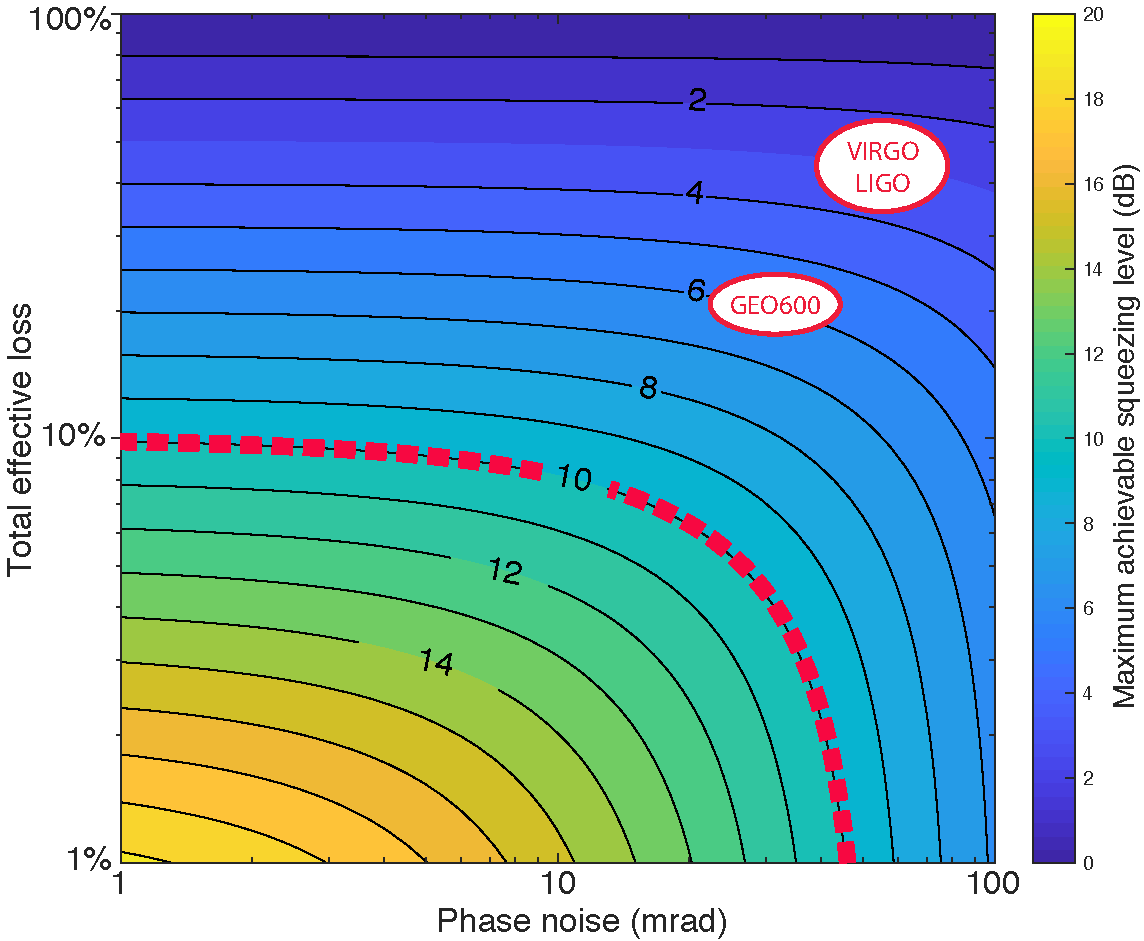
\includegraphics[width=0.5\textwidth]{./Detector/DetFigures/QNSQZvsPNandLoss.pdf}
	\caption{Maximum effective squeezing level as function of phase noise and optical loss. In order to reach the goal of 10\,dB detected squeezing, the optical loss needs to be smaller than 10\,\% while the phase noise must not exceed 10\,mrad.}
	\label{QNSQZvsPNandloss}
\end{wrapfigure}
%
The current generation of detectors achieve their exquisite sensitivity due to their kilometre-scale arm lengths, the enormous light powers circulating in the enhancement resonators (arm, power- and signal-recycling cavities), and sophisticated pendulum suspensions that isolate the test mass mirrors from the environment. When these techniques were developed, squeezing was not envisioned to become an integral part of such a system. However, the sensitivity improvements achieved already today via the injection of squeezed light (as an upgrade / add-on) are significant. For GEO\,600 an effective squeezing level of 6\,dB has been detected in the shot noise limited frequency band. As shown in Fig.\ref{QNSQZvsPNandloss} this corresponds to 25\,\% optical loss with a phase jitter of the squeezing ellipse of around 30\,mrad. A further reduction of optical loss and phase noise, the improvement in mode matching of the squeezed field to the interferometer signal field and mitigation of polarization mismatches will improve the effective quantum noise reduction even more in the future.
%
During the O3 science run both Advanced LIGO detectors and the Advanced VIRGO detector have not only been limited by quantum shot noise at high frequencies but have also operated close to being limited by quantum radiation pressure noise at lower detection frequencies. As a consequence, the injected squeezing level can not be increased to improve the high frequency sensitivity without degrading the detector sensitivity at lower frequencies and vice versa. 
%
It was revealed by Unruh~\cite{Unruh1982} and others~\cite{Yuen1983, Pace1993} that squeezed field injection with frequency dependent squeezing angle allows an overall quantum noise reduction including the radiation pressure noise thereby beating the standard quantum limit (SQL). The effect of a simultaneous suppression of quantum noise by means of a frequency dependent orientation of the squeezing ellipse (i.e. the correct squeezing phase for all detection frequencies) is illustrated in Fig.~\ref{UnruhFDS}.
%
%
\begin{wrapfigure}{l}{0.5\textwidth}
	\centering
		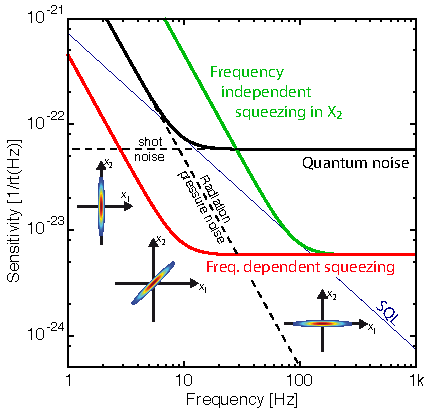
\includegraphics[width=0.5\textwidth]{./Detector/DetFigures/UnruhFDS.pdf}
	\caption[Illustration of frequency dependent and independent squeezed light injection]{Illustration of frequency dependent and independent squeezed light injection.}
	\label{UnruhFDS}
\end{wrapfigure}
%
For Advanced Virgo and Advanced LIGO, this can be realized with a detuned filter cavity and the corresponding technology is currently under development and planned to be implemented before the science run O4.  
%
The ET detectors will be quantum noise limited over the entire detection band and therefore suitable filter cavities have to be implemented. For the squeezed light injection into an optical spring interferometer, an additional rotation of the squeezing ellipse is caused first by the phase-space rotation of a detuned cavity and second due to the optical spring resonance. In this case at least two filter cavities are necessary to achieve a broadband reduction of quantum noise with squeezed states of light. This is what we propose for the low-frequency ET-LF interferometer (cf. Sec.~\ref{sec:xylophone}). For the high-frequency ET-HF interferometer one filter cavity is enough (cf. Sec.~\ref{sec:xylophone} and \cite{Hild2010b}).

The filter cavity assisted rotation of the squeezing ellipse has been experimentally demonstrated
in table top experiments both at MHz ~\cite{Chelkowski2005} and kHz \cite{Oelker2016} frequencies. However,
(0.1--1)\,km class filter cavities are required for long arm interferometers. For this reason a first prototype based on a 300\,m cavity is currently under test at the National Observatory of Japan (NAOJ) with the aim to obtain a rotation at approximately 70\,Hz ~\cite{Capocasa2019}.
Both collaborations LIGO \cite{McCuller2019} and VIRGO \cite{Degallaix2019} are presently working on the development of cavities of the same length scale. In general the optimal cavity length and parameters depend on the interferometer configuration. In this section we summarize the methods used for optimizing the filter cavities to be implemented in ET.

The use of filter cavities along the optical path of the squeezed light induces additional mechanisms and sources of squeezed light degradation which are in general frequency dependent. In optimizing the cavity design these detrimental effects must be taken into account: 

\textit{Filter cavity round trip loss --} The most relevant squeezing degradation mechanism comes from the filter cavity round trip losses which induce two effects: first optical loss mixes non-squeezed contributions into the squeezed vacuum state which leads to a degradation of the resulting squeezing level. Second the presence of filter cavity losses combined with the frequency dependent reflectivity mixes the two quadratures thereby corrupting squeezing with anti-squeezing. This effect cannot be compensated by a rotation of the state and therefore definitively deteriorates the actual quantum noise reduction ~\citep{Kwee2014}. To limit the impact of these effects the relevant parameter to be minimized is the cavity round trip loss per unit length $l^2_{rt-fc}/L_{fc}$ \cite{Khalili2010}. Therefore in order to keep the filter cavities length to an acceptable value the round trip losses must be minimized. 
% 
\begin{figure}%[ht]
\centering
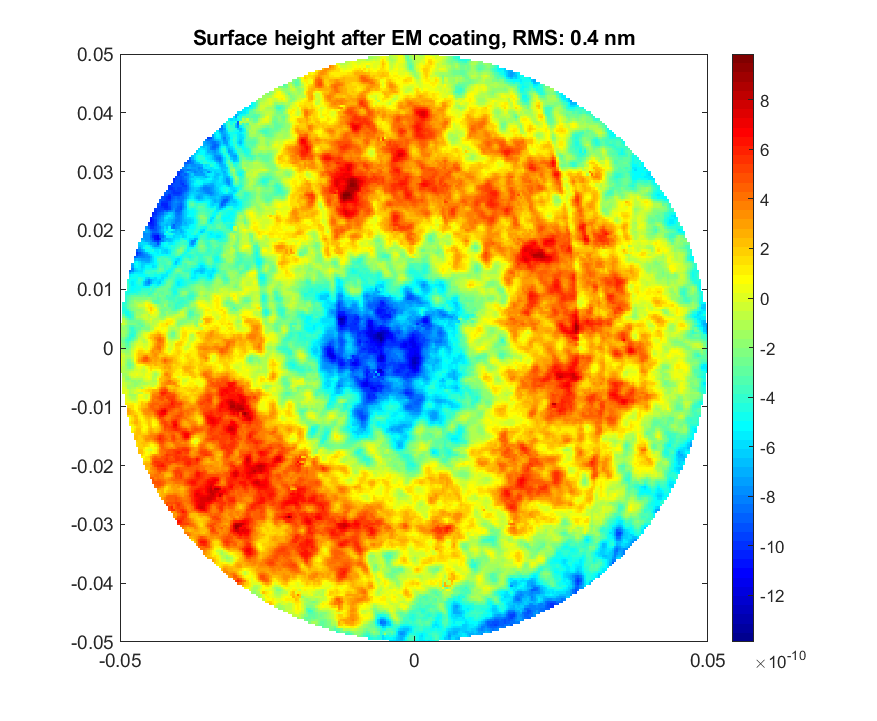
\includegraphics[width=68mm]{./Detector/DetFigures/Mirror_Map.png} 
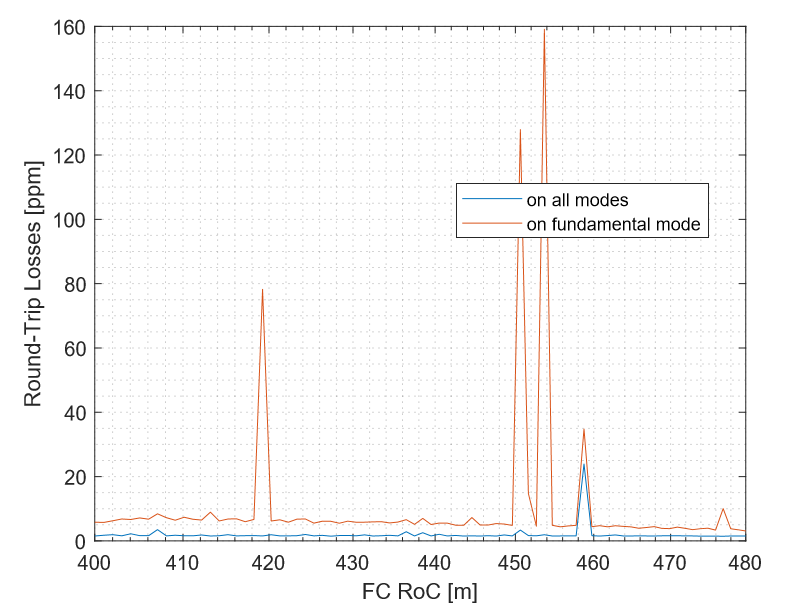
\includegraphics[width=75mm]{./Detector/DetFigures/FC_Stray.png}
\caption{{\it Left}: Virgo end  mirror surface map. The elements of the map represent the surface height deviation from a perfectly spherical mirror in meters ({\it provided by J. Degallaix/LMA}). {\it Right}: Expected cavity round trip losses as a function of the radius of curvature (RoC) of the mirrors for a 500\,m long linear cavity, equipped with Virgo-like mirrors (left plot) 200 mm in diameter ({\it credits M. Eisenmann)}. The background value derives from the light scattered outside the cavity, while the peaks originate from scattered light that couple to the high order modes of the cavity. The calculation is based on the method used in Ref.\citep{Capocasa2016} }
\label{fig:FC_rt_strain}
\end{figure}
%
Round trip cavity losses ($l^2_{fc-rt}$) are generally dominated by light scattering on the cavity  mirror surfaces. For this reason among the possible filter cavities configurations the {\it linear} cavity, which minimizes the number of mirrors, is preferable \cite{Evans2013}.  Recent measurements show that 50--90\,ppm can be achieved in 300\,m long linear cavities \citep{Capocasa2018}, a similar result (<60 ppm) has been obtained  for the VIRGO long arms.  Moreover, in the near future a further decrease in the scattering losses is foreseen. Indeed a numerical calculation shows that  with the latest  mirror quality and by optimizing their  diameter and radius of curvarure, scattering losses for a 500\,m long cavity can be constrained to 5--10\,ppm ( Fig.\ref{fig:FC_rt_strain} {\it right}).
%
In this design report we assume for the cavity round trip losses the ultra-conservative value $l^2_{fc-rt}=75$ ppm. However, to illustrate also lower cavity losses Fig.\ref{fig:FCoptimization} shows the quantum noise reduction, which can be expected for filter cavities with round trip losses in the range 40--75\,ppm. 
%
\begin{figure}%[htbp] \centering 
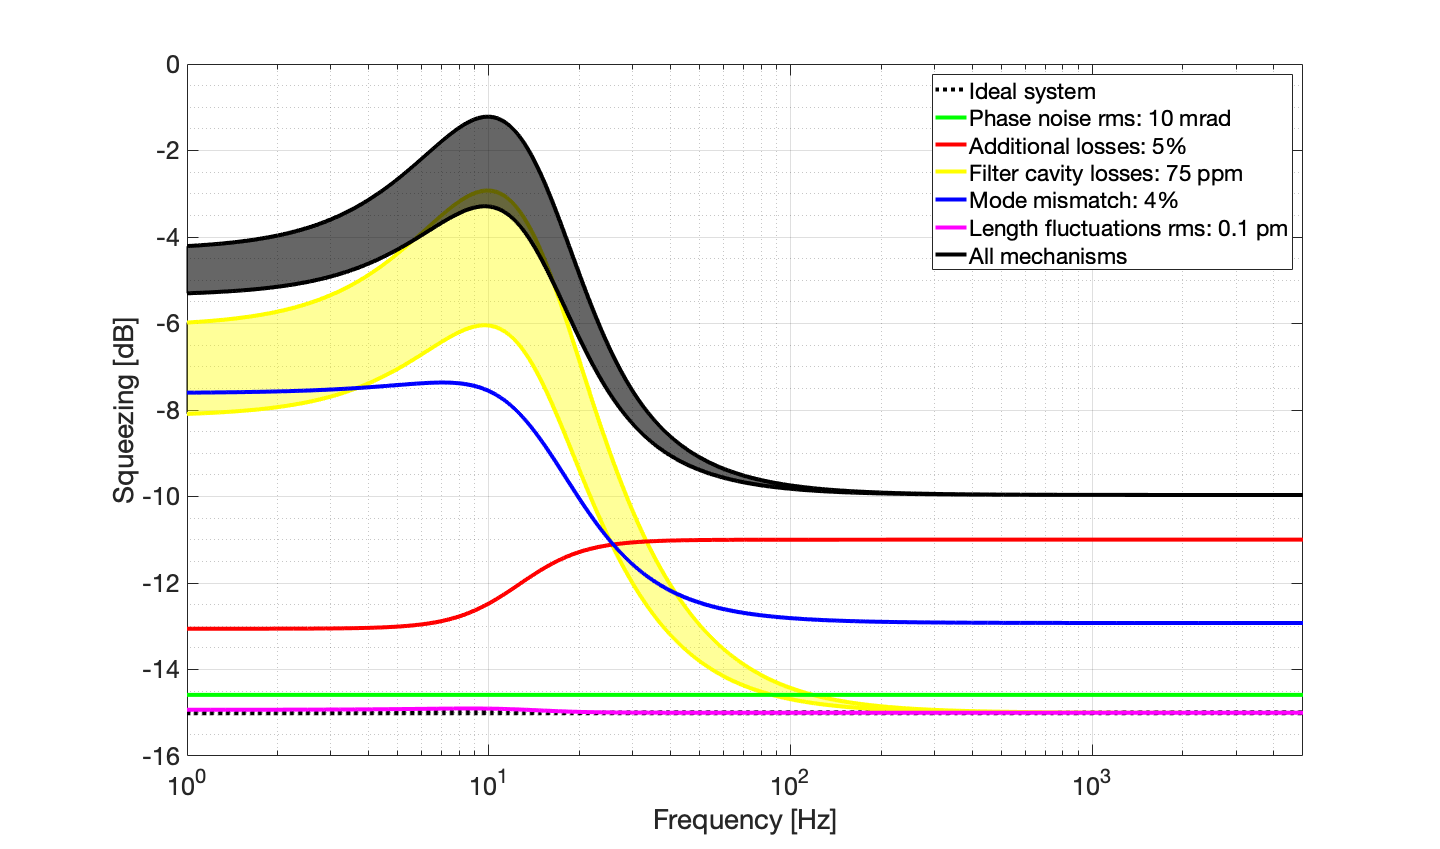
\includegraphics[width=77mm]{./Detector/DetFigures/ET_FC.png}
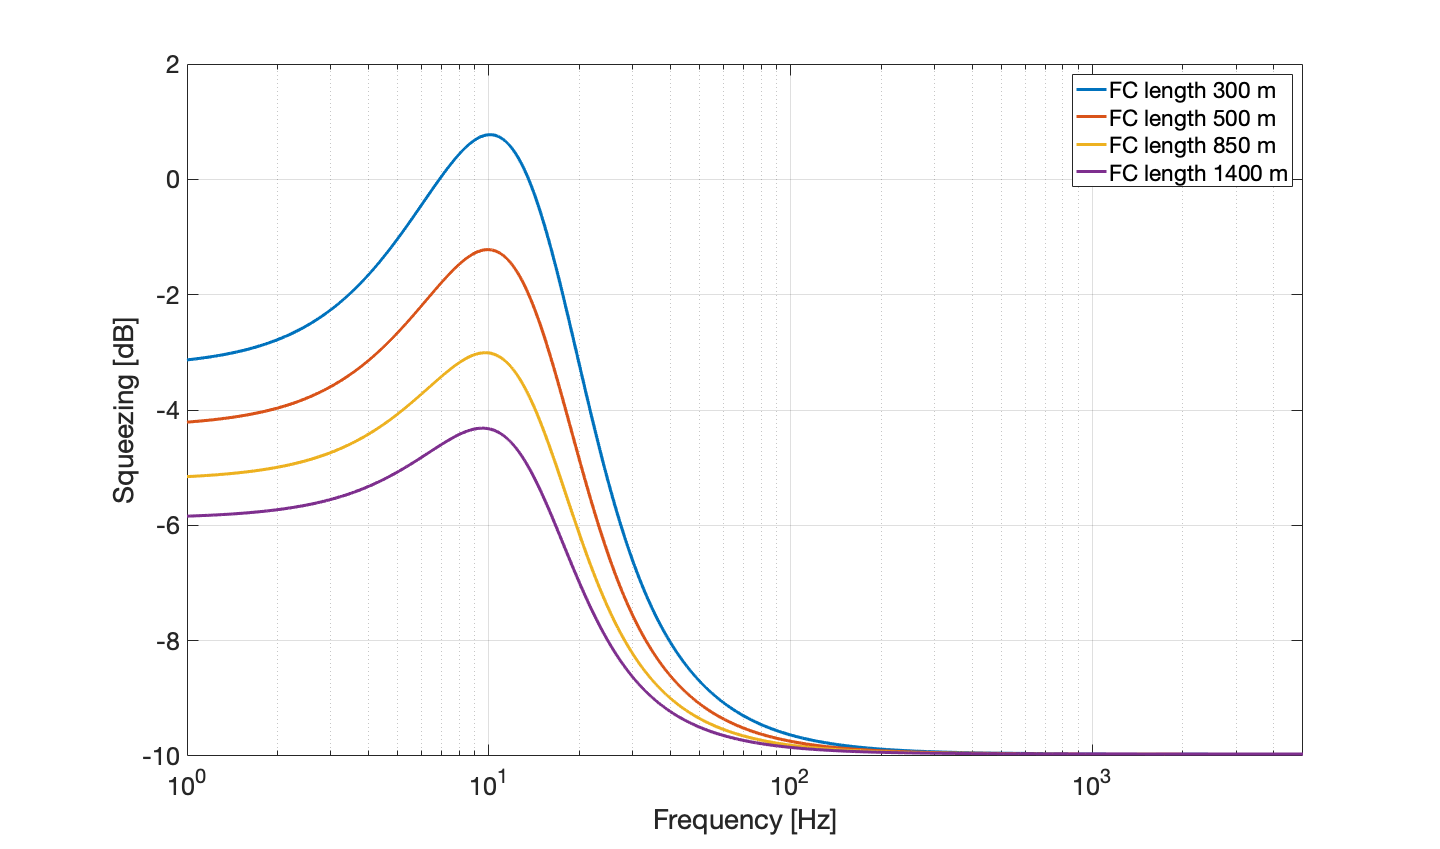
\includegraphics[width=77mm]{./Detector/DetFigures/FClength.png}
\caption{ {\it Left:} Ratio between the quantum noise with and without squeezed light injection for a 500\,m long cavity. Several (colored curves) degradation mechanisms contribute to the total squeezing degradation budged (black curve). The dominant contribution at low frequencies derives from the round trip losses of the cavity (yellow curve). The values assumed for the cavity round trip losses range from 40\,ppm to\,75 ppm. {\it Right:} Total degradation budget for different cavity lengths ({\it credits E. Capocasa}).} 
\label{fig:FCoptimization}
\end{figure} 
%

\textit{Mode mismatch --} A non-perfect spatial overlap (mode mismatch) between the squeezed beam and the eigenmode of the filter cavity
 is a source of optical loss, which is independent from the filter cavity length. 
 The target mode matching value of ET is $\sim 98\%$, analog to the LIGO and VIRGO quantum noise reduction projects.

\textit{Phase noise --} The achievable sensitivity improvement by injecting squeezed light is deteriorated due to phase noise between the interferometer carrier and the squeezed field. The suspended filter cavity can produce phase noise due to residual changes of the cavity length $\delta L_{fc}$ which generate fluctuations in the detuning frequency $\Delta \omega_{fc}$:
%
%Except for intra-cavity fluctuations phase noise is in general frequency independent.  
%A typical intra-cavity fluctuation is generated by the residual displacement noise $\delta L_{fc}$ of the cavity length which generates fluctuations in the detuning frequency $\delta \Delta \omega_{fc}$.
%
  \begin{equation}
    \delta \Delta \omega_{fc}=\omega_0 \frac{\delta L_{fc}}{L_{fc}} \ .
  \end{equation}
For this work we assume $\delta L_{fc}=0.1$\,pm. which is  within the reach of current technologies.

Figure \ref{fig:FCoptimization}-{\it left} shows the level of quantum noise reduction as a function of frequency for the ET-HF configuration. %(table...). 
The optimal cavity bandwidth $\gamma_{\rm fc}$ (half-width at half-maximum) and detuning $\Delta \omega_{\rm fc}$ are calculated analytically according to Ref. \cite{Kwee2014}. 
Figure \ref{fig:FCoptimization}-{\it right} shows that the quantum noise reduction increases by extending the cavity length. However, this effect is less and less pronounced as one approaches frequencies beyond the cavity bandwidth, where the sources for squeezing degradation are filter cavity length-independent. Moreover, at low frequencies additional technical noise sources contribute significantly to the overall detector sensitivity and thus a strong quantum noise suppression is not observable and hence not required. A short cavity design is therefore well suited for an efficient high frequency quantum noise reduction, with a reduced suppression at low frequencies. This strategy also minimizes the costs and complexity and is therefore applied to the ET-filter-cavity designs.

A similar optimization was also used for the two cavities of the detuned configuration as planned for ET-LF. However, to our knowledge in this case no analytical expression for the optimal cavity bandwidth and detuning is available in presence of losses. Therefore the optimization was done numerically. 
This optimization process led to the choice of a length of 500 meters for the ET-HF filter cavity and 1000 meters for the two ET-LF cavities.
\label{Sec:FDS}
% Autors: Jean-Pierre Zendri, Moritz Mehmet, Henning Vahlbruch


%\subsection{Auxiliary Optics}
\input{Detector/Optics/AuxOptics/AuxOptics.tex}

\subsection{Interferometer control}
% Author: Hartmut Grote



To operate GW interferometers such as ET, many degrees of freedom (DOFs) need to be controlled. 
The most important DOFs belong to the interferometer as a whole, and can be divided into the longitudinal DOFs, which involve controlling the position of the main mirrors along the optical axis, and the angular DOFs which refer to the orientation of the main mirrors with respect to the incident beam axis. 
There are several more control loops, the auxiliary loops, which control e.g. the position or velocity of some part of a suspension, or the power of the laser system, but we mostly focus on longitudinal and alignment control here, since these are most critical for the overall performance of the interferometer.

Regardless of the split in longitudinal and alignment control,
some links between them exist too, such as the bi-linear coupling of alignment control noise with
beam spot position on test masses into the longitudinal signals. We will point these out where required.


\subsubsection{Longitudinal control}

In the steady-state operation of the interferometer, longitudinal control is concerned with maintaing longitudinal DOF's relevant to keep the interferometer and optical cavities at (or sufficiently close to) their nominal operating points. Another distinctive task of longitudinal control is lock acquisition, which is the process of bringing the interferometer reliably to its steady-state operating point.

For a single Fabry-Perot cavity, consisting of two or more mirrors, the standard way to obtain an error signal for locking the cavity to resonance with the incoming laser light, is the Pound-Drever-Hall technique \cite{Drever1983}. The technique consists of adding RF sidebands to the optical frequency of the laser using a modulator. Alternatively modulation can also be applied to the cavity itself, e.g. by modulating the round-trip length of the cavity. The signal in reflection of the cavity is then demodulated yielding a signal proportional to the deviation from resonance. This error signal can be used to control the length of the cavity by e.g. actuating on the mirror, or to control the laser frequency. This is a system with a single DOF and is applied for input mode-cleaners and output mode-cleaners of current GW interferometers, with sufficient performance to also be suitable for ET.

A GW interferometer is more complex than a single cavity, and has more longitudinal degrees of freedom. 
The number of DOF's for the main interferometer is determined by the number of optical resonators that form
the interferometer (plus one for controlling the interference condition of the Michelson interferometer). Typically there are more suspended mirrors than DOFs which leaves some of them uncontrolled, as for example a global translation of all mirrors or the relative position of folding mirrors within recycling cavities (the latter may be controlled for ET if required, to reduce scattered light from moving fringe patterns on folding mirrors).

The first generation ITFs (called PRFPMI), such as initial LIGO and Virgo consisted of 4 DOFs: Differential Arm length (DARM), consisting of the length difference of the two long arm cavities, Common mode ARM length (CARM), the length sum of the two long arms, the Michelson DOF (MICH) and the Power Recycling Cavity Length (PRCL). For the second generation detectors advanced LIGO, advanced Virgo and KAGRA, a fifth DOF is added: Signal Recycling Cavity Length (SRCL), which will also be the case for the ET interferometers.

%[xx figure with DOF definition, ports]

Of these five DOFs, the DARM loop is of particular importance, since it directly contains the information of gravitational wave signals. This means that greatest care is taken to bring the noise performance of the corresponding readout to the most fundamental limits of the given configuration.
Since this DOF is also actively controlled, the effect of the corresponding feedback loop must be taken into account to obtain a calibrated gravitational-wave signal that can be used for data analysis.

The operation of the Advanced LIGO and Advanced Virgo interferometers
has demonstrated the feasibility of longitudinal control techniques for second generation detectors.
In particular advanced LIGO, since operating with a signal recycling (extraction) mirror from the beginning,
has demonstrated the control scheme for five longitudinal degrees of freedom,
including their lock acquisition. 
The basic scheme is based on the Pound-Drever-Hall technique, but uses two sets of modulations simultaneously,
which are designed to yield signals for all five DOF's by sensing different combinations of the sideband signals and the carrier light at different interferometer ports \cite{SensingStrain:2003}.

Ideally one would obtain one error signal per DOF, which is only sensitive to that DOF. In practice most signals are sensitive to more than one DOF, but to varying degrees. 
The situation is coped with by using multiple-input, multiple-output (MIMO) linear combinations of signals 
as well as gain hierarchy. Feed-forward/noise subtraction for spurious couplings is employed as outlined below.
The ET design will build on this scheme, using simulations to find optimal sets of modulation frequencies and detection ports.

The operation of Advanced LIGO has shown that coupling of residual motion of the signal recycling cavitiy length to the main gravitational wave readout (DARM degree of freedom) is a limitation
of the sensitivity at low frequencies if DC readout is used. Since this coupling is proportional
to the offset chosen in the DARM DOF,
in ET this limitation will be avoided with the use of balanced homodyne detection (BHD) \cite{frit2014}, as also foreseen for the LIGO upgrade A+ currently under development.
The employment of a BHD readout scheme for ET makes the optical layout a bit more complex, but the requirements seem well understood at this time. Experience at LIGO will inform the BHD design for ET.


All currently operating interferometers employ digital control loops wherever possible, for the benefit of flexibility, stability and transient noise reduction of control transfer functions. Typical sample frequencies are around 10-64 kHz, but even for faster loops digital control is now used (at Virgo the fastest digital loop is now at 500 kHz.) 

Digital demodulation is a technique that has been used in advanced Virgo, where optical signals are sampled with very high frequencies (several 100 MHz) in order to perform demodulation operations digitally, rather than with analog mixers \cite{TheVirgo:2014hva}. Recent advances in high-speed ADCs and FPGAs allows this option. This technique maintains flexibility throughout this signal processing step, at the cost of more complex hardware and need for careful dynamic range design. The benefits probably outweigh the disadvantages, such that the application of this technology for ET seems likely. The experience with advanced Virgo is a valuable input here.

%The holometer was using FPGAs and might have used even faster loops, to be checked)

%Several ways of obtaining error signals

%2) For the 2nd generation, the readout of the sensitive DARM DOF was changed from an RF signal to using \emph{DC detection}. In this scheme, the DC power of the asymmetric output is used for DARM. Since this has a zero slope exactly at \emph{dark fringe} condition, a small offset (either to DARM or MICH) must be used. This system is more sensitive due to XX [cite DC detection]

%3) for future detectors (e.g. LIGO O5?), even another scheme might be used, in which the AS port is interfered with a reference beam, this is known as balanced homodyne. No offset is needed in this case, which has xx advantages.

\subsubsection*{Lock acquisition}

One challenge of operating a GW interferometer is that at the operation point (steady state), several cavities need to be simultaneously resonant with picometer accuracy, while in the uncontrolled interferometer the mirrors are freely swinging by up to a micrometer per second. This already assumes that the payloads are pre-stabilized using the \emph{local controls}, which are part of the suspension system. Since the ET interferometers have 5 DOFs, the phase space is enormous.

For systems with 3 DOFs, this problem is still manageable (e.g. GEO lock acquisition), since one can simply wait a short while until the various DOFs are close to resonance by chance, and then switch on the control loops with appropriate triggers (e.g. on some cavity power). However, already for GEO auxiliary locking signals derived from modulation sideband power had to be used. For 4 DOFs it gets harder, but was achieved with Initial LIGO \cite{Evans2002}, in which various loops are switched on in short succession, while changing the sensing scheme on the fly. Instantaneously locking 5 DOFs at about the same time is very hard due to the enormous phase space. It had successfully been tried out at the Caltech 40\,m prototype, 
but was ultimately judged too unreliable.

At the Virgo interferometer, the problem of locking 4 DOFs was tackled in a different way, by locking individual DOFs sequentially at different working points, before deterministically transitioning to the final one in several steps. This technique is called Variable Finesse \cite{VariableFinesse}, since it initially locks the Michelson DOF at half-fringe, thereby making it an effective mirror with low reflectively. 
In the initial state the power recycling mirror is misaligned and gets slowly aligned during the locking sequence. This technique has been perfected over the last 10 years at Virgo and works very reliably.
It may be possible that such a technique can be extended to 5 DOF's, by initially misaligning PRM and SRM mirrors, to be suitable for ET, but this will need more simulation work.

For Advanced LIGO, as a result of the difficulty locking the 5 DOF configuration, an auxiliary laser system (ALS) was developed, which can lock the arm cavities independently with a different laser \cite{LIGO_ALS1, LIGO_ALS2}.  The technique used for aLIGO is to use an independent green laser system, which can lock the arm cavities and keep them out of resonance for the IR, while the remaining 3 central DOFs are locked in a traditional, one-shot way. Green laser light is injected from the end, and then extracted in central and interfered with the frequency doubled PSL.

%[figure ALS scheme, maybe from Martinov paper]

Locking a DRFPMI using ALS has been successfully demonstrated with the Advanced LIGO interferomter \cite{aLIGO_lock_acquisition}, which is now in daily use. For the KAGRA detector it is foreseen to use a similar scheme, but with the green injected from the central area towards the end. If this works, this would be a nice simplification of the LIGO scheme \cite{KAGRA_ALS}.
It still employs additional hardware though, which also need additional time for commissioning and maintenance. Therefore, if a reliable locking system can be found without using an ALS it would clearly 
be preferable in order to keep all systems at the lowest required complexity level.


\subsubsection*{Steady state control}

Once all the degrees of freedom are controlled and moved to their final working point, all control signals are derived from error signals with the lowest available noise (the highest signal-to-noise ratio). Further, control loops get optimised and actuator dynamic ranges get reduced, to minimize or eliminate digital-to-analog conversion (DAC) noise. When reached, this can be called the steady state, in which the most sensitive gravitational-wave measurements are performed. 

In the steady state, noise of control loops gets important. Noise is being introduced to the interferometer's DARM DOF (which carries the GW signal) by longitudinal and alignment control loops. Typically this 'control noise' is dominated by the sensing noise of the contributing loops.
Control noise is very relevant for ET, where one of the biggest challenges is to move the lower frequency limit of the detection band down from around 10-20 Hz (is current detectors) to 4 Hz. This is a frequency region where control noise from angular and auxiliary longitudinal DOFs typically dominates the sensitivity.

For the auxiliary longitudinal DOF's (MICH, PRCL, and SRCL) noise subtraction schemes are employed
successfully for the 2nd generation detectors, forming the model for ET.
The methods can be divided in \emph{online} and \emph{offline} methods.
Online methods work in real-time while the interferometer is operating,
subtracting a sample of the auxiliary loop feedback from the DARM signal by
applying it to DARM actuators with appropriate filtering.
Offline methods subtract properly filtered feedback signals form auxiliary loops
from DARM, after the DARM signal has been recorded.
%online: alpha note, vajente locking paper, something at ligo
%offline: Meadors, Driggers, 
%Hrec. Might need something non-linear like latest thing by Gabriele
Novel non-linear noise subtraction methods are under development, and possibly can
improve subtraction performance for ET.



%reducing noise of DARM loop is fundamental, but this is usually based on fundamental noises, or technical noise sources, and typically not on 'control noise' (i.e. changing the feedback filter does not change the calibrated output of the ITF). Aux DOFs need be clean too, due to the finite coupling to DARM. In this case, also the shape of the loop, or the accuracy is important, which can be called control noise. This influence needs to be minimized by careful optimization of the loops, and by subtracting (online or offline) any noise that remains.
%reduction of control noise of aux DOFs



%SRCL: tuned/detuned ...

%\subsubsection*{new techniques}



%SRCL control through the dark port: [cite thesis Vaishali Adya]

%balanced homodyne (cite Fritschel et al) might be the future. this will likely be tested in one of the next upgrades at LIGO for O5 or O6, so this might be a mature technology at the time of ET.

%suspension point interferometry?






\subsubsection{Alignment control}

Alignment control is primarily concerned with keeping all optics aligned with respect to each other
and with respect to laser beams propagating between the optics.
As such, it is global in the sense that it uses interferometric information about the relative alignment
of laser beam axes, predominantly obtained with differential wavefront sensing (DWS). 
In addition to this, alignment control is also concerned with keeping beam spots at dedicated positions (preferably close to the center) on the interferometer mirrors. This is a secondary goal, referred to as spot position control, that uses local information obtained from beam spot position sensors or from alignment (dither) modulation schemes. In the following we will be only looking at DWS alignment issues.

As for longitudinal control, alignment control for ET will be based on the successful alignment
solutions existing for advanced LIGO and advanced Virgo.
For differential wavefront sensing, these are based on the extended Pound-Drever-Hall scheme as devised for longitudinal control,
using at least two optical modulation frequencies and several sensing ports.

However, since alignment control noise is limiting sensitivity at low frequencies in advanced LIGO and Virgo, (e.g. below about 20\,Hz in LIGO during the O3 run in 2019 ), 
improvements will be needed for ET.

A lower alignment control noise can be achieved in two major ways, namely by 
\begin{itemize}
\item reducing the residual alignment-relevant motion of the optics, i.e. motion 
without the engagement of global alignment control
\item increasing the signal-to-noise ratio of the alignment (DWS) sensing signals
\end{itemize}

Advances in the sensing and control of the suspension for ET will lead to some reduction of the alignment motion of the optics. Tilt-meters can be used to break the degeneracy of tilt and acceleration sensing at low frequencies, or novel seismometer configurations (6-d seismometer) may be used to this end \cite{MLMa2018,YuHM2018}. 
If lower suspension (and thus mirror alignment) motion is achieved, this can be used for a reduction of alignment feedback bandwidth, thus lowering DWS control noise.
For the ET-HF interferometer such potential reduction of bandwidth may be limited by
the optical alignment springs (caused by radiation pressure, i.e. the Sigg-Sidles instability),
which may require damping with DWS alignment control of sufficient bandwidth.
Due to operating at lower laser power, in the ET-LF interferometer the optical alignment springs will be at lower frequencies than for ET-HF, such that a lower DWS control bandwidth may be realised here.
What helps in case of ET-HF though is that the problem of alignment feedback noise is less severe in the first place. Due to the choice of sensitive frequency band, the interferometer can tolerate more low-frequency control noise than the ET-LF interferometer. Here the xylophone design of ET is clearly of advantage \cite{Hild2010a}.
Further, the increase of mirror masses to 200\,kg for ET (about 5 times more than advanced detectors)  
helps with decreasing the alignment optical spring frequencies.
There may also be alternatives to damping of alignment optical spring resonances with DWS feedback,
which is to be investigated. It may be possible to damp such modes with radiation pressure of the laser light itself, applying feedback forces in a narrow frequency band. This may help to reduce control
noise originating from the DWS sensors if a bandwidth reduction is possible.

It is expected that the increase in beam size in ET will make the alignment requirements more severe
than for 2nd generation interferometers [?].
Ultimately, the more detailed technical design studies have to account for this, and a find a suitable
compromise.

Improvements in the signal-to-noise ratio of alignment sensing signals are currently more uncertain.
As a benchmark, new systems would have to have sensing noise below $10^{-15}$ rad/$\sqrt{\rm Hz}$,
to make substantial improvements, which needs some more R\&D.
The planned BHD readout will help in reducing contribution to sensing noise on wavefront-sensor signals, since it removes the first-order coupling of beam position on the wavefront sensor into the alignment signal.

Another (additional) way to reduce alignment control noise coupling to DARM is to develop (possibly non-linear) Wiener filtering, to subtract alignment feedback noise using known witness channels. Some of these implementations have successfully reduced noise at operating interferometers. 



%\subsubsection{Detection?}

%\subsubsection{Calibration}


%\subsection{Alignment and beam shape control}
%\tcb{does not exist yet}
% merge 

\subsection{Scattered Light Mitigation Systems}
% Author: Antonino Chiummo
\subsubsection*{Introduction}

Stray-light in gravitational-wave interferometric antennas is the light coming from the laser source which does not follow the intended path. The reasons for that deviation could be many, such as scattering off non-idela surfaces of optical elements, clipping by finite aperture, spurious reflections off anti-reflective surfaces and so on. Stray-light related noise has been recognized to be an issue since the very first investigation of technical limitations in the interferometers designed for detection of gravitational waves \cite{Billing79}. A tiny amount of stray light coupling with the fundamental mode after probing the vibrations of infrastructures will bury any gravitational signal. \\
Let us indicate by $f_{sc}$ the fraction of laser power that couples back to the main interferometer mode $\Psi_0$ after a scattering event:
  \begin{equation}
    f_{sc} = |\langle \Psi_{stray}|\Psi_0^*\rangle |^2
  \end{equation}
 The overall field will then be expressed by the superposition of the these two contributions: 
   \begin{equation}
        E_{tot} = E_{in} + E_{s} = E_{in} + \sqrt{f_{sc}} E_{out} e^{i \phi_s(t)}
   \end{equation}  
where $E_{s} = \sqrt{f_{sc}} E_{out} exp \left[i \phi_s(t) \right]$ is the scattered field in the main mode.
The whole point about the issue of the stray light is all in the phase modulation of the stray field due to the motion $ z_s(t)$ of the stray source:
   \begin{equation}
        \phi_s(t) = \phi_0 + \frac{4\pi}{\lambda} z_s(t)
   \end{equation}
  This modulation of phase is not only directly mimicking a gravitational wave signal if it leaks to the anti-symmetric port of the interferometer, but also can give rise to \textit{amplitude noise} of the field \cite{vajente_vesf12}:

  \begin{equation}
        E_{tot} = E_{in} \exp \left[ \sqrt{f_{sc} \frac{P_{out}}{P_{in}}} \left( cos \phi_s(t) + i sin \phi_s(t) \right) \right]
  \end{equation}
  To be noticed that the above equation holds true for whatever amplitude of stray light source motion, provided that the fraction of stray light is such small to be treated as a perturbation. Nevertheless, when such motion is large with respect to the field wavelength $\lambda/2$, important non-linear effects emerge due to the \textit{fringe wrapping} of the phase modulation.\\
The problem of stray light could therefore break down to understand and possibly mitigate:
\begin{itemize}
    \item the recombination $ f_{sc}$ of stray light to the main mode;
    \item the amplitude and frequency of the displacement noise $z_s(t)$ of the stray light source;
    \item the transfer function of the stray field to the anti-symmetric port of the interferometer.
\end{itemize}
\subsubsection*{Lessons learned}
The first studies on the potential impact of stray light were performed by K. Thorne back in 1989 \cite{Thorne89}, followed soon by J.Y. Vinet, S. Braccini and V. Brisson. The main goal was to assess the impact and the possible mitigation of stray light bouncing in the long arm tubes \cite{Vinet96, Vinet97}. The outcomes of the studies were both the design (geometry, position, materials) of a system of baffles to be installed in the long tubes, and the translation of Monte Carlo methods to track photons in the GW community. This latter method, however, was soon understood not to be enough to fully capture the potential risks of the stray light, without taking into account the coherent effects that were not easy to simulate.\\ This scenario changed with the development of simulation methods based on Fast-Fourier Transform applied to laser field propagation \cite{SIS,DarkF}.



%**********************************************
\FloatBarrier
%\section{Seismic Isolation and Suspension}
% Authors: Giovanni Losurdo, Giles Hammond, Conor Mow-Lowry
\label{Sec:SASandSUS}

\subsection{Seismic Isolation Systems}
\label{Sec:SAS}
\label{sec:seismic}

%\tcb{first draft C Mow-Lowry/G Losurdo Nov 2019}

{\bf Overview of seismic isolation}

The seismic isolation system fulfills three main functions:
\begin{itemize}
    \item to suppress the seismic noise below the sensitivity requirements in the detection frequency range (for ET at frequencies larger than 1-2 Hz);
    \item to reduce the RMS input motion to the suspension systems, particularly at the suspension resonances and the micro-seismic peak(s);
    \item to provide large-scale and slow position control of the test-masses.
\end{itemize}

Two main concepts have been implemented so far in GW ground-based detectors:
\begin{itemize}
    \item The Virgo Superattenuator \cite{};
    \item The Advanced LIGO HEPI/ISI \cite{}.
\end{itemize}

Both of them rely on a combination of passive and active isolation, but the approach is substantially different. The Superattenuator is mostly based on a passive approach to seismic noise suppression, thanks to a design characterized by very low normal mode frequencies, whereas it needs active control for RMS reduction. On the contrary, the Advanced LIGO system makes use of an aggressive control strategy to "dig" actively into the seismic noise.


{\bf ET baseline}

The baseline for ET, defined in the 2011 CDR and detailed there, consists in using a longer Virgo-style Superattenuator. The increased length (17 m) allows to reduce the normal mode frequencies and push the seismic wall down to $\sim$2 Hz. 

The main advantage for such a choice is that it provides a design thoroughly tested during many years of operation in Virgo and which requires only minor R\&D to be adapted to ET: it therefore represents a safe pathway towards a 3G configuration. 

\paragraph{SA modifications for Low Frequency ET}

In order to extend the detection bandwidth of the Einstein Telescope in the low-frequency region starting from a couple of Hz, a better seismic attenuation in the ultra-low frequency range is needed. To this purpose a detailed simulation devoted to this design study was performed for the 2011 ET Conceptual Design. The SA dynamics in the low frequency range, where the inner normal modes of the mechanical filter chain are confined, was simulated by using the electro-magnetic equivalent circuit (a series of oscillators). 
A maximization algorithm, called \emph{Simplex}~\cite{Different2008_SecondEdition}, based on the possibility to change the masses and the mechanical filter chain lengths, was developed. It searches for a maximum attenuation performance at a fixed frequency that, in our case, was 2\,Hz.  Since the transfer function has a smooth shape, it turns out that to get a higher attenuation at 2\,Hz, we should have a lower  "cross-over frequency" with the requirements curves (see Fig.~\ref{Par4Fig1}). As showed in the direct measurement performed with the Virgo interferometer (see section 4.1.1.c), the cross-over between seismic noise at the mirror level and the requirements is dominated by the residual horizontal seismic vibrations. For this reason to move the cross-over at lower frequency, we need to improve  the attenuation performance of the horizontal seismic vibration in the low frequency range.
%
\begin{figure}[t]
	\begin{center}
		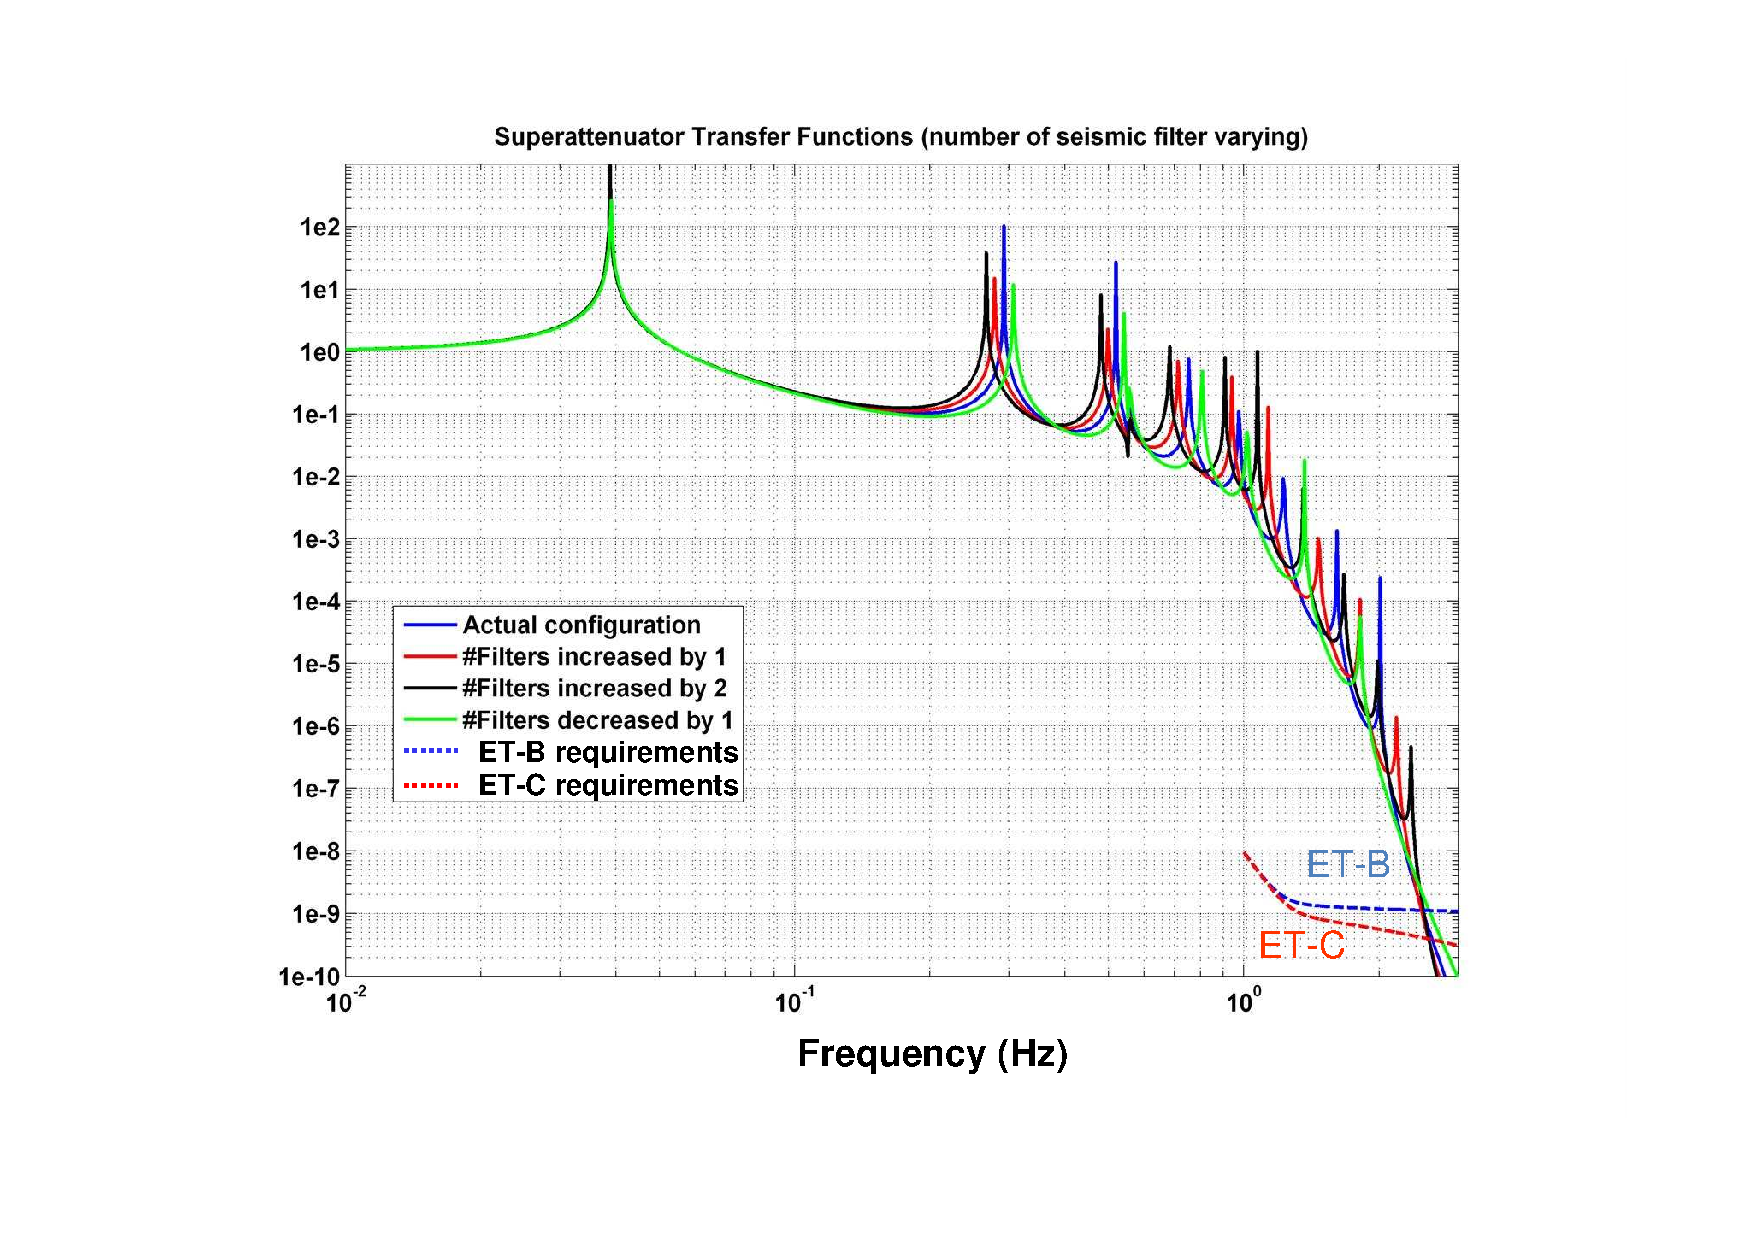
\includegraphics[width=0.9\textwidth]{Detector/SASandSUS/SuspensionSystems/Suspension_Figures/Par4-Fig1.pdf}
			\caption{Simulation results of the SA horizontal transfer function with the present chain length (9 m). Changing the number of (``equal-spaced'') filters the resulting horizontal transfer function is compared with the ET requirements (for High Frequency---\emph{ET-B}---and low frequency or ``xylophone'' configuration---\emph{ET-C}). Adding or removing filters along the chain length do not have remarkable role in the positioning of the cross-over frequency with the requirements.}
\label{Par4Fig1}
	\end{center}
\end{figure}
%
An important preliminary conclusion of the abovementioned design study is that, fixing the length and the number of mechanical filters, the optimal configuration (i.e.\ that one minimizing the cross-over frequency or maximizing the attenuation performance at 2\,Hz) is that one where the filters are separated along the chain by the same distance. This "equal-spaced" configuration represents the optimal one even because the vertical transfer function is not influenced by the filter positioning along the chain. Moreover it has been proved that increasing\,/\,decreasing the number of filters or changing their masses does not play a fundamental role in determining the cross-over frequency between the horizontal transfer function and the requirements. The results obtained are plotted in Fig.~\ref{Par4Fig1} and Fig.~\ref{Par4Fig2} while in the corresponding captions complementary information is available.  
%
\begin{figure}[t]
	\begin{center}
		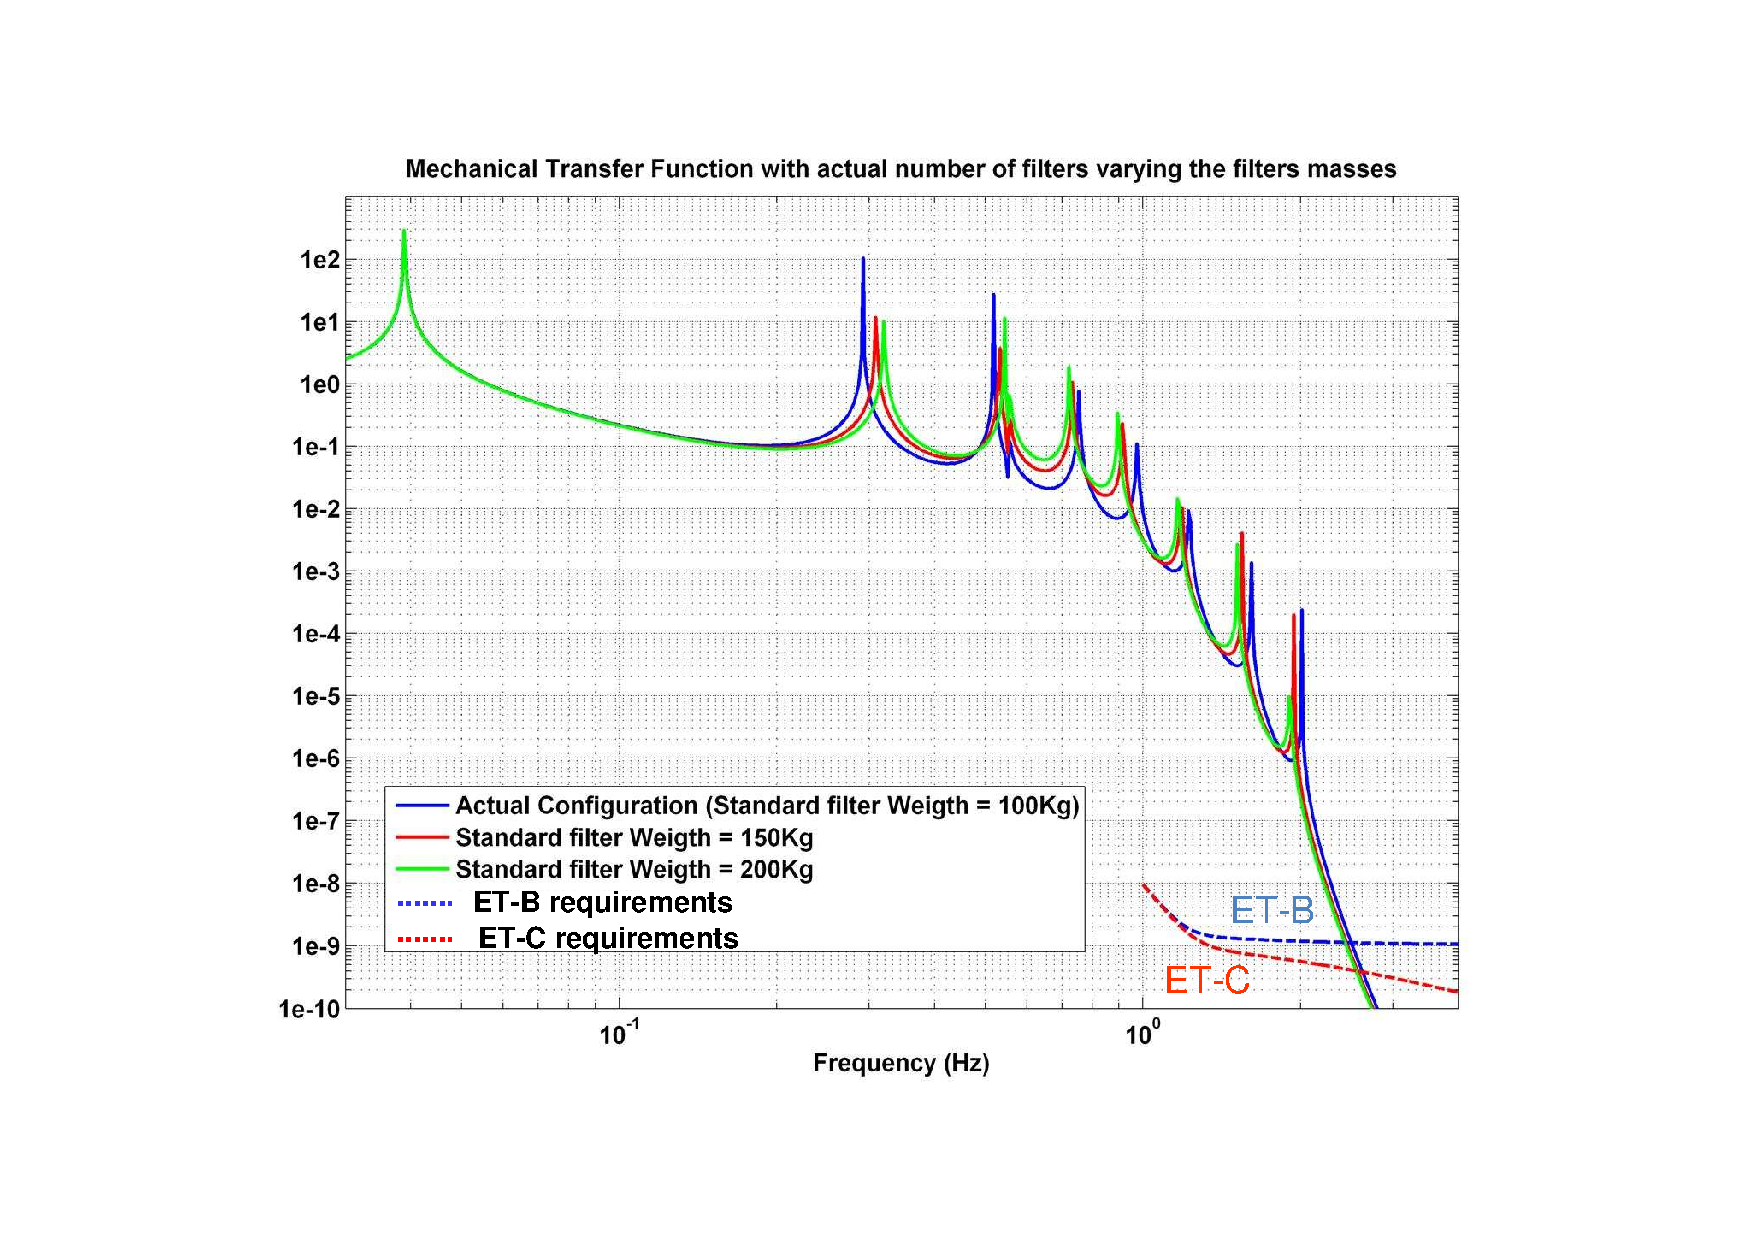
\includegraphics[width=0.9\textwidth]{Detector/SASandSUS/SuspensionSystems/Suspension_Figures/Par4-Fig2.pdf}
			\caption{The horizontal transfer function of the present \emph{SA} (6 filters weighting 100\,kg each one for a total length of about 9\,m) is compared with the same transfer function changing the mass of each filter (150\,kg and 200\,kg). Also in this case the cross-over frequency with the ET requirements is not remarkably affected by the change of the filter mass.}
\label{Par4Fig2}
	\end{center}
\end{figure}
%
\begin{figure}[t]
	\begin{center}
		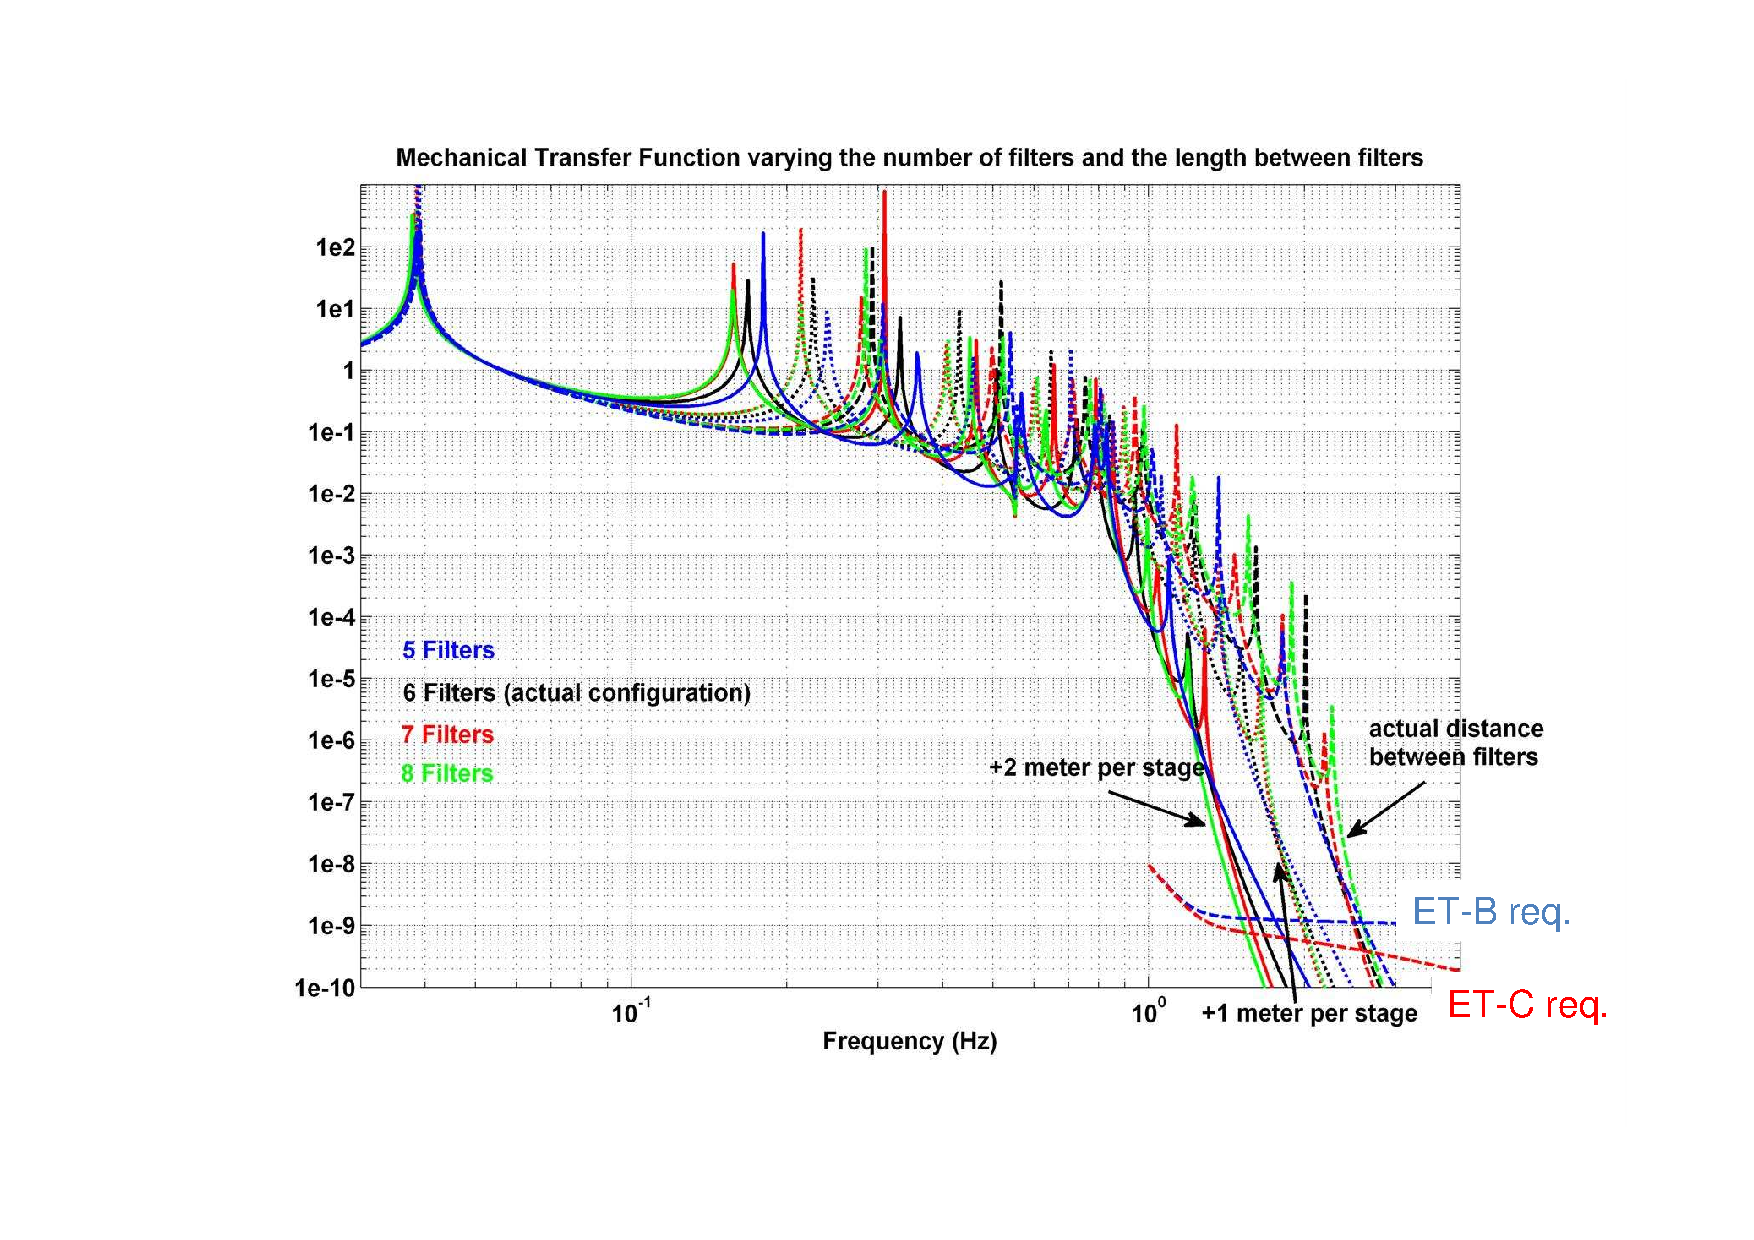
\includegraphics[width=0.9\textwidth]{Detector/SASandSUS/SuspensionSystems/Suspension_Figures/Par4-Fig3.pdf}
			\caption{Simulation results for different configurations. The horizontal transfer function of the \emph{SA} is plotted changing the number of filters and keeping fixed their relative distances ("equal-spaced" geometry) along the chain (changing, as a consequence, the full length of the SA).}
\label{Par4Fig3}
	\end{center}
\end{figure}
%
The only way to move in the low frequency region the cross-over frequency extending the Einstein Telescope bandwidth below 3 Hz, is to increase the SA chain total length. The simulation results for different configurations can be found in figure~\ref{Par4Fig3} and described in~\cite{Braccini2010March1-3}, while the best solution seems to be represented by a SA with 6 filters and a total length of 17\,m (identical the Virgo configuration, where 5 mechanical filters suspended from an horizontal pre-isolator stage plus the marionette are assembled forming a filter chain about 9\,m long). As shown in Fig.~\ref{Par4Fig4}, with this solution the cross-over frequency has been placed around 1.7--1.8\,Hz, that is considered enough for our purpose. Indeed, Newtonian noise and other technical noise are assumed to prevent an effective detection above a couple of Hz.
%
\begin{figure}[t]
	\begin{center}
		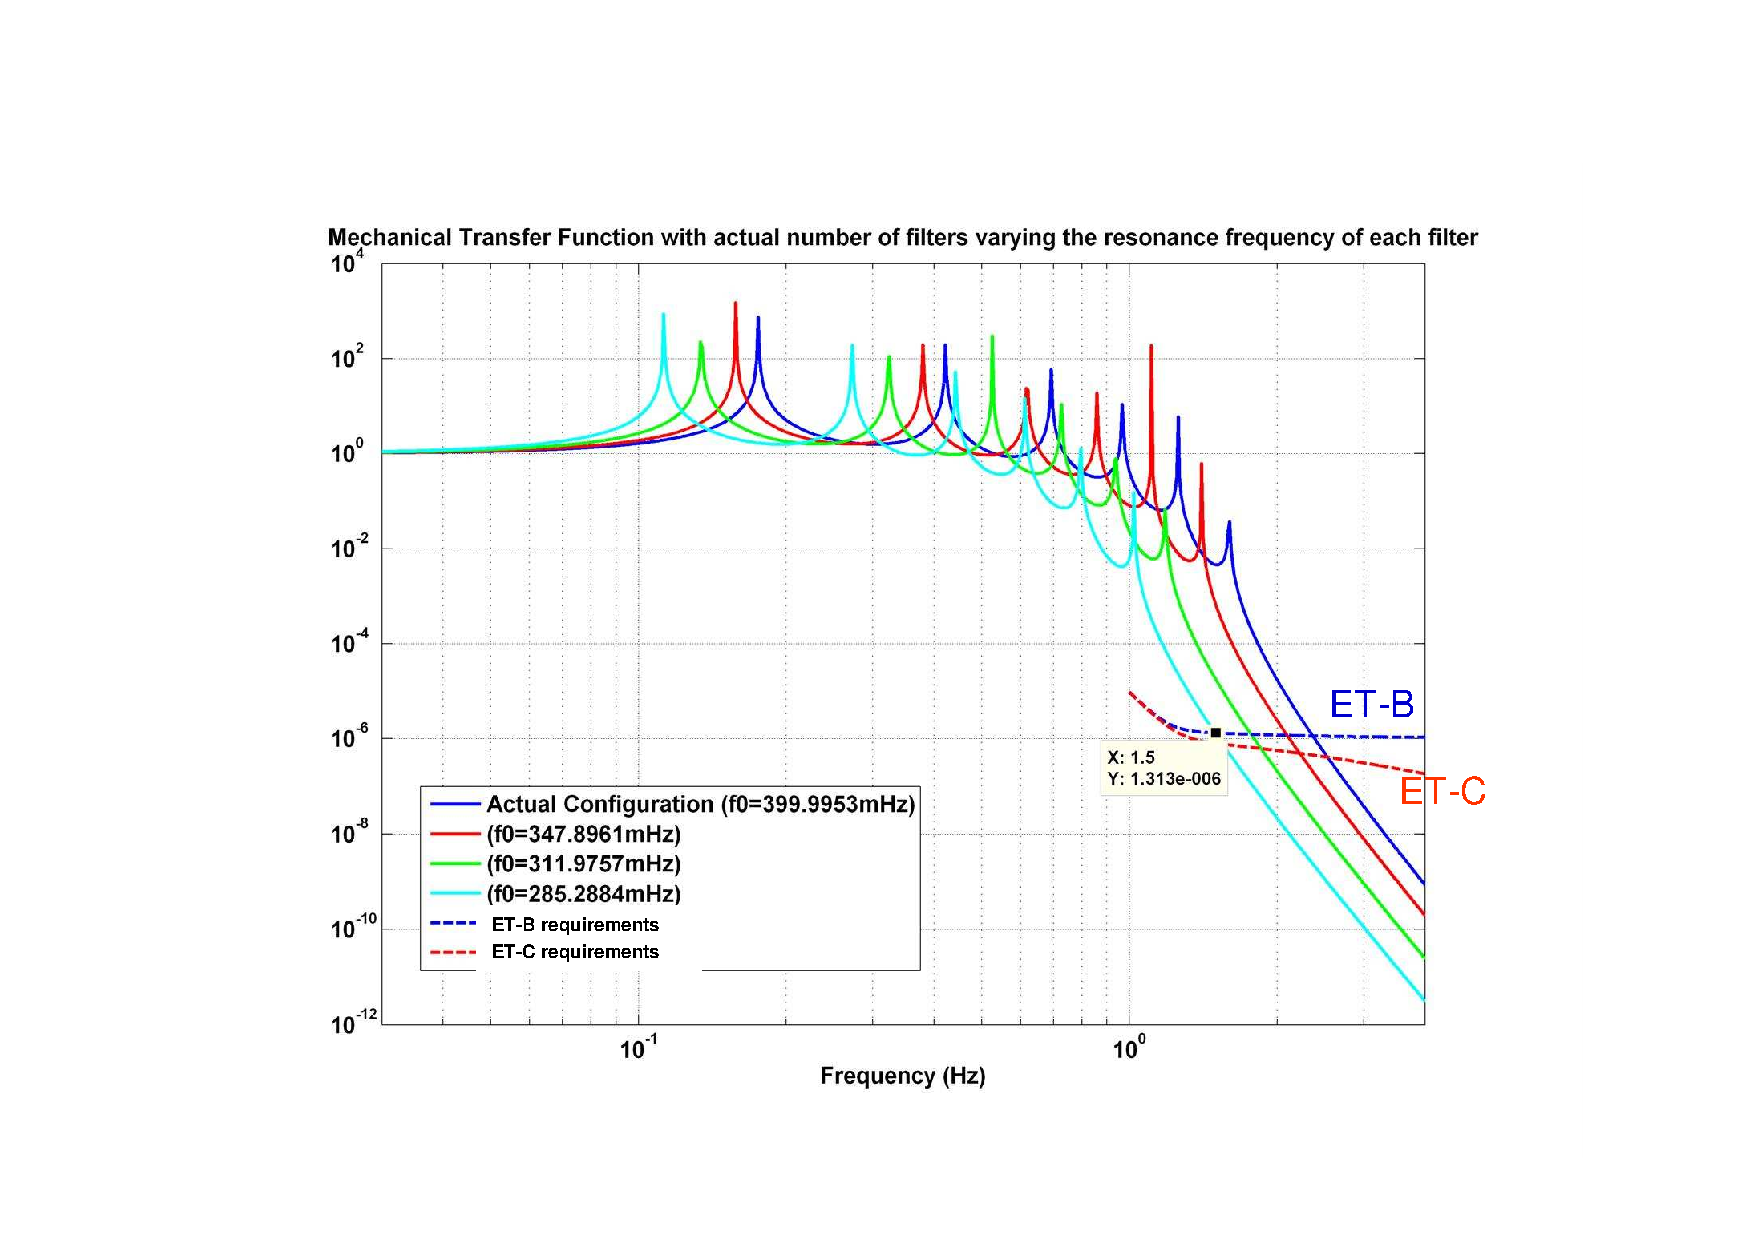
\includegraphics[width=0.9\textwidth]{Detector/SASandSUS/SuspensionSystems/Suspension_Figures/Par4-Fig5.pdf}
			\caption{Vertical Transfer Function of the SA considering the six stages (as it is now, i.e.\ with the pre-isolator or ``Filter Zero'' plus other five mechanical filters). The different curves have been obtained changing the filter vertical resonant frequency. With filters working around 300\,mHz it is possible to move the cross-over below 2\,Hz.}
\label{Par4Fig5}
	\end{center}
\end{figure}
%
With this configuration, the vertical cut-off frequency of the whole system is set below 1.8\,Hz by tuning each mechanical filter having the main vertical frequency around 300\,mHz (see Fig.~\ref{Par4Fig5}). The corresponding vertical transfer function is plotted in Fig.~\ref{Par4Fig4}. Since the residual seismic noise along the vertical direction, at the level of the mirror, is expected to limit the Einstein Telescope sensitivity again around 1.7--1.8\,Hz, a coupling factor of $10^{-3}$ has been considered. This is due to the fact that the Earth curvature makes plumb lines at a 10\,km distance not parallel each other. At least one mirror has to be inclined with respect to the local plumb line performing the alignment of the cavities. This transmits the residual vertical mirror motion along the beam with the mentioned coupling factor ($10^{-3}$).
%
\begin{figure}[t]
	\begin{center}
		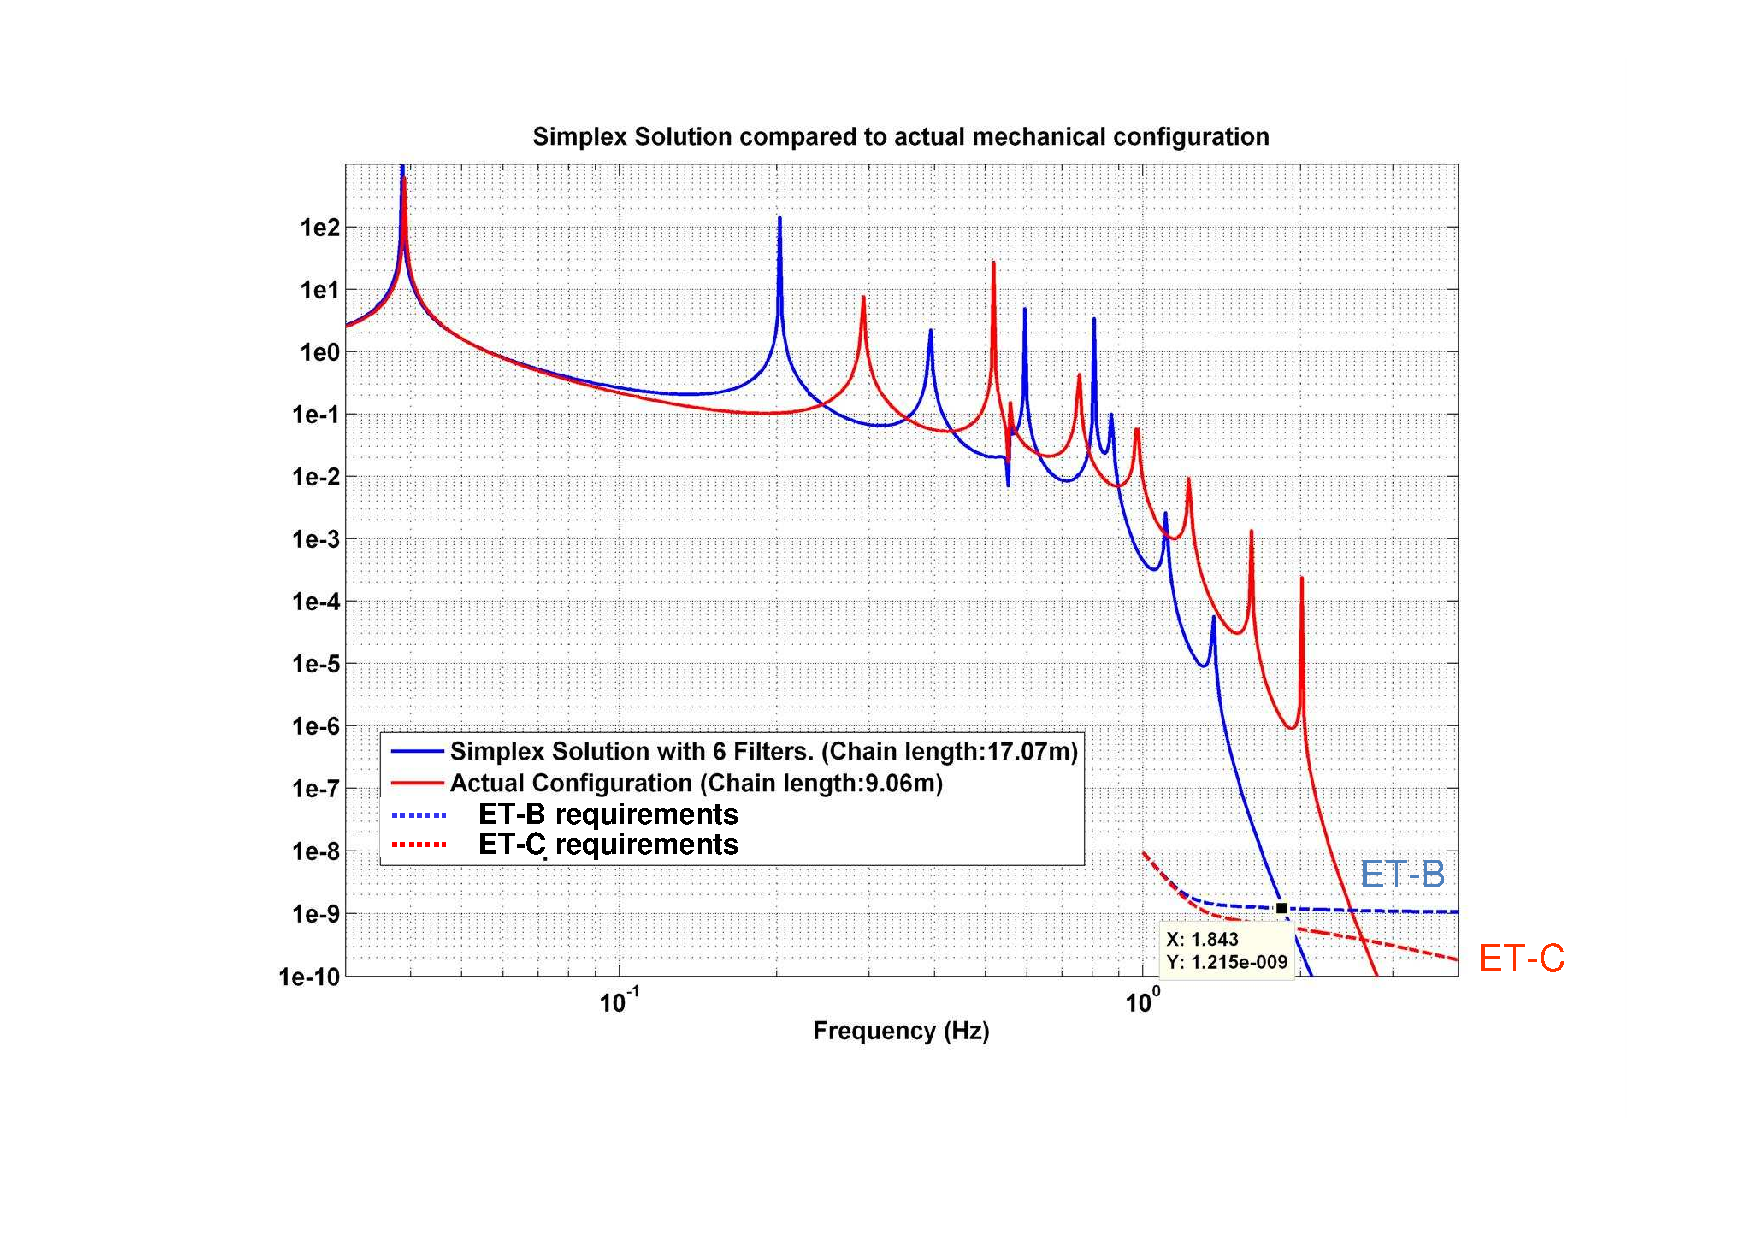
\includegraphics[width=0.9\textwidth]{Detector/SASandSUS/SuspensionSystems/Suspension_Figures/Par4-Fig4.pdf}
			\caption{The proposed reference solution for the $SA$ configuration of the Einstein Telescope. Other slightly different configurations are discussed in \cite{Braccini2010March1-3}.}
\label{Par4Fig4}
	\end{center}
\end{figure}
%
Since years in Virgo many mechanical filters with a cut-off frequency of around $300$ $mHz$ \emph{Superattenuators} are  in operation  with an excellent stability. By using the Virgo interferometer data, it has been observed that the long-term change of the chain main resonant frequencies induced by the temperature variation under vacuum are 
well inside the line-width of the chain vertical resonances. No effect on the interferometer control is due to this potential disturbance. Moreover, even if the temperature variations induce a motion of the suspension chain and then a slow vertical displacement ({\it {breath}}) of the mirror (a few $mm$ per $^{\circ}C$ is the measured 
value for the Virgo \emph{Superattenuator}), this effect is well within the specifications of any interferometer (vacuum tank provides an excellent temperature stability - fraction of $^{\circ}C$ peak to peak).
The standard SA, presently in operation on the Virgo interferometer, is already well inside the third generation specifications from this point of view too.

In addition, it is important to remind that the requirements in the tens of Hz range are less stringent in Einstein Telescope than in Advanced Virgo (see section 4.1.1.a) and thus, fixing to six (a choice lead by the reduction of the cross-over frequency) the number of filters, a better attenuation performance in the high frequency range is not necessary anymore since the safety margin is large enough in Advanced Virgo and even larger in an underground environment. In conclusion, a SA $17$ $m$ high with 6 magnetic anti-spring filters ("equal-spaced" configuration) tuned with a vertical cut-off frequency around 300 $mHz$, represents the reference solution for the Einstein Telescope. 

{\bf Possible alternatives to the baseline}

There are two main reasons which push for seeking a different approach:
\begin{itemize}
    \item the 17m Superattenuator is not sufficient to push the seismic wall down to 1 Hz, which is the ET target;
    \item it could be convenient to reduce the Superattenuator height to ease the constraints on the height of the caverns.
\end{itemize}


A possible alternative to be investigated could be coupling a Superattenuator to an inertial platform controlled in 6 d.o.f.: this configuration would make use of a combination of the technologies and expertise developed in the GW field so far. One could imagine, for instance, the inertial platform being the base of the Superattenuator. This kind of approach was envisaged already in Virgo: the Superattenators are realized on a rigid platform resting on 3 elastic feet which can be actuated by piezos. This had been designed in order to be able to perform an active control of the ground tilt. The ET design should extend this concept in order to allow also for horizontal control.




%{\bf Mechanics of the suspension upper stages}

%The suspension upper-stages are primarily required for the reduction of input vibration within the sensitive band. They are also often used for actuation and damping. 

%\textit{In Virgo, this is all filters between Filter Zero and the Marionette, in LIGO this is the 'top' and 'UIM' masses of the Quads.}



{\bf Sensor development}

The seismic isolation systems will require the development of new sensors not currently deployed in-vacuum. At the minimum, this will include some kind of inertial rotation sensor to enable tilt-control at frequencies at and below the micro-seismic peak, and displacement sensors to allow damping of suspension modes without injecting noise.
In general, the lower seismic noise intensity in the underground site will naturally require accelerometers with a lower proper noise. 



\subsection{Test Mass Suspension Systems}
\label{Sec:SUS}
https://www.overleaf.com/5857319888dfyxsfqvsgpx

hal: this url does not exist. Did you mena:
https://www.overleaf.com/project/5d40a8fe67993a7c805ef910 ?
\FloatBarrier

\section{Cryogenics}
%author Fulivi Ricci 
\label{Sec:Cryogenics}
\subsection{The ET cryostats}
\label{subsec:cryo}
In order to limit the thermal noise impact on the ET sensitivity curve it is necessary to cool at cryogenic temperature the four test masses of the LF-detector. The heat is extracted from the mirror via the suspension fibres attached at the other end to the marionette. Moreover, the marionette is suspended to the super-attenuator which attenuates the seismic noise up to few hertz. Thus, it is extremely important at the same time (i) to preserve the mechanical isolation between the mirror and the cooling system, (ii) to guarantee an efficient thermal link between the payload and the cooling system. 

% In figure%~\ref{fig:cryo_infrastructure_figure/ET_main-cryostat}
% we report a sketch of the cryo-mechanical system to be adopted for ET-LF. 

\begin{figure}[h!]
	\centering
		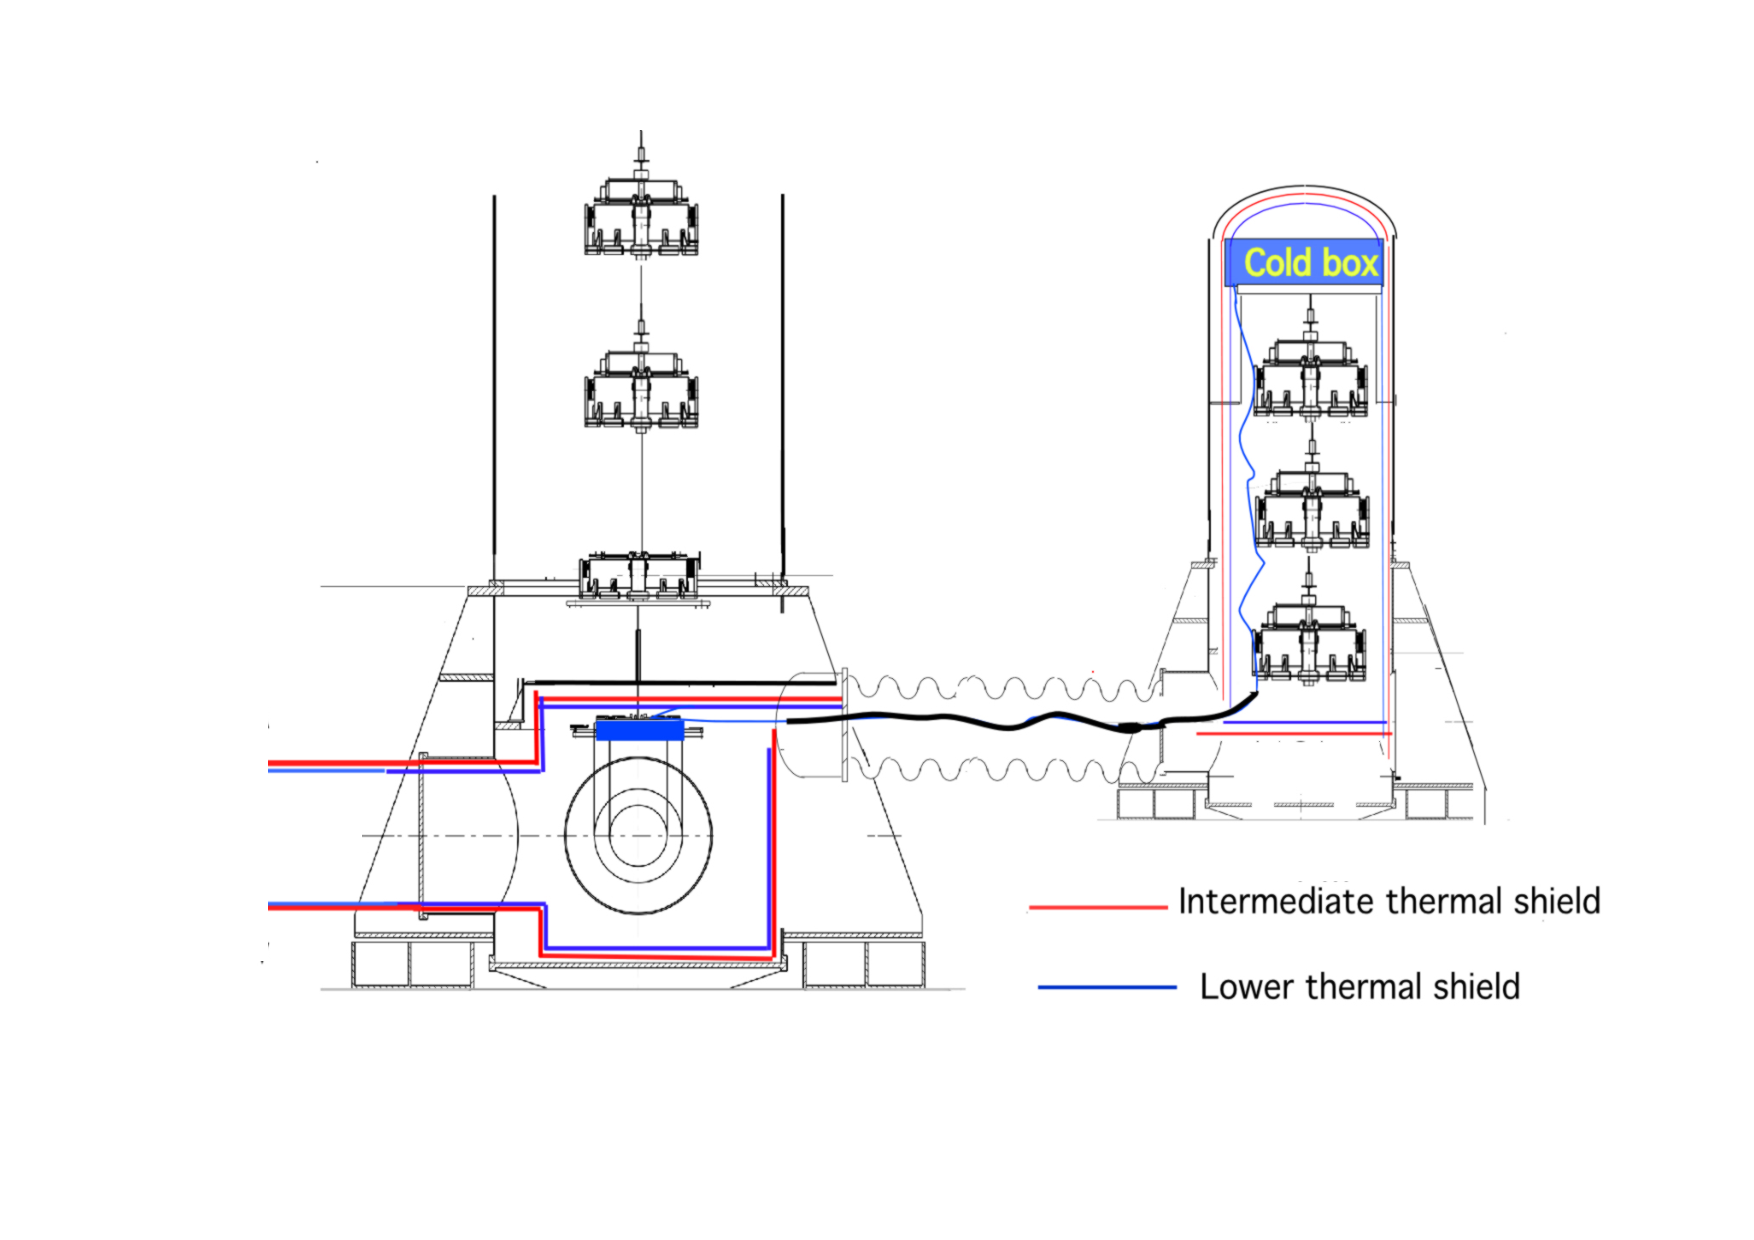
\includegraphics[width=0.9\textwidth]{./Intro/Intro_Figures/ET_main-cryostat.pdf}
	\caption{Scheme of the cryostats needed for cooling a test-mass of the LF-interferometer.}
\label{fig:cryo_infrastructure_figure/ET_main-cryostat}
\end{figure}
\redcomment{hal: will this figure be replaced by a newer one?}

The whole payload is housed in the lower part of the vacuum tower hosting the 17-m long super-attenuator chain. The base of the vacuum tower is a cryostat with two thermal screens: the blue line schematizes a surface at $\sim4$\,K, while the red line represents the shield at intermediate temperature ($\sim 80$\,K). The upper part and lower part of the tower are separated by a roof crossed by the Ti-6Al-4V thin rod which holds the whole payload
%\footnote{The interface between the upper and lower suspension is described in section~(\ref{Upper_lower_suspension_interface}.}. 

The blue line defines a volume that has to be vacuum-tight. It will permit to cool-down and warm-up faster the whole payload by adding pure Helium gas in this experimental volume. 
\redcomment{which volume? How is it separated against the rest?}
Few mbars of helium will provide an efficient heat exchange during the cooling phase of the payload from room to cryogenic temperature. Once the equilibrium temperature is achieved, the helium gas is pumped out before the laser light injection. 

The base of the main tower hosting the mirror is connected to an ancillary tower shown in the figure+\ref{fig:cryo_infrastructure_figure/ET_main-cryostat}. The ancillary tower  hosts the cold box, which will keep the mirror at cryogenic temperature. 
%The cold box can be either a simple liquid helium container in the case of a cryoplant based on cryofluids or the cold head of a cryo-refrigerator in the case of a cryocooler plant. 
A thermal line of $\sim 20$ m length connects the cold box to the last stage of the mirror suspension. It can be made of a braid of a high purity material as the electrolytic copper or the grade 6 aluminum (99.9999 \% purity). Both of them are metals characterized by thermal conductivity value of 2 kW/m/K in the range 1-10 K. In fact a braid of 20 m length, made of 8 wires 1 mm diameter can support an heat flow of 200 mW for a temperature difference of$\sim$ 1K at the link ends. To damp the vibration associated to the cooling system, the soft braid is mechanically coupled to the auxiliary super attenuator chain, hosted in the ancillary tower and fully complaint with the cryogenic environment. In order to define the requirement of the cryo plant we have to estimate the cryostat thermal inputs, which depend on the cryostat dimension and the quality of the thermal insulation. \noindent Assuming that the inner vacuum chamber has to host a mirror with a half meter diameter, we derived the order of magnitude of the thermal input for the cylindrical cryostats whose dimensions are reported in the following table: 
\begin{table}[htp] 
\caption{Cryostat dimensions} 
\begin{center} 
\begin{tabular}{|c|c|c|} \hline \hline Container & Diameter [m] & Height [m]\\ \hline Payload vacuum chamber & 1.5 & 3 \\ Auxiliary tower & 1 & 2 \\ \hline \hline
\end{tabular} 
\end{center} 
\label{tab:cryostat_dimension} 
\end{table} 

The thermal super insulation is a standard technique used in the modern cryostats. The thermal shield is formed by highly heat reflective thin layers, set under vacuum for increasing radiation reflection and decreasing radiation heat transfer through the insulation. The most known implementation is based on layers of porous (self-vented) mylar sheets, which are aluminized on one side. The sheets are wrapped around the surface to be insulated and form a multilayer blanket. The mylar is an hydroscopic material incompatible with the HUV requirements of ET. As a consequence the proposed solution implies to separate the chamber hosting the mirror to the insulation vacuum of the cryostat. A dedicated pumping system ( rotary-roots-turbo-molecular group) will provide the vacuum insulation. Wrapping 25 and 75 layers of self vented aluminized mylar around the two thermal shield, we achieve the condition to limit the thermal input below 1\,W for the 4\,K shields and around 50\,W for the intermediate ones. We assume in this evaluation that the thermal input due to laser light absorbed by the mirror and the thermal radiation emitted by the the km tube is in the range of few tens of milliwatts thanks to low silicon absorption at the laser wavelength and to the helium cryotraps described above
%in~\ref{subsection_helium_cryotraps}
. It is worthwhile to evaluate these data in more detail as part of the ET technical design study.  

\subsection{The LF-interferometer cryotraps}

\subsection{The cryogenic fluid distribution plant}
\label{subsec:cryo_distr_plant}
Cryogenic fluids in the form of liquid helium and liquid nitrogen are required to circulate for cooling the cryostats of the test masses and the associated cryotraps. The heat load requirement at a particular temperature is a prime important factor to select a helium refrigerator/liquefier and to define the dimensions of the nitrogen plant. The cryogenic systems of ET should operate in different modes cool down, steady state and warm up for each test mass tower, The cooling time is a trade off between the need to limit the detector down time and the stress due to the thermal gradients During cool down the recommended flow rate of helium gas will be approximately $\sim 1$\,g/s. The heat load requirement of cryogenic systems including the transfer loss at steady state is approximately $\sim 20$\,W at 4\,K helium refrigerator/liquefier. A helium refrigerator/liquefier having refrigeration capacity of 160\,W at 4\,K in refrigerator mode and 50\,L/h in liquefier mode without LN2 pre-cooling and 200\,W at 4.5\,K in refrigerator mode and 100\,L/h in liquefier mode with LN2 pre-cooling, is sufficient to guaranty the cooling in the vertex area of the triangular interferometer. In this evaluation a redundancy factor has been included so that the system will satisfactorily cater the refrigeration load at different state. As we anticipated before, to reach a full flexibility of the system, the possibility of performing the cool-down and the regeneration with the main refrigerator has been foreseen too. The cryogenic system will include a distribution valve box and the cryogenic piping up to the interface of the ET cryostat. The distribution valve box contains a 1000 L liquid helium control dewar, a heat exchanger, an electrical heater, a Joule-Thompson cryogenic valve and relevant instrumentation for pressure, temperature and flow rate measurements. The cryogenic system has to deliver, in a controlled way, the cooling helium from the refrigerators to the client. It includes mainly a 80\,K gas helium circuit and a 4.5\,K helium circuit, that can be interconnected through bypass valves; both shut-off valves and control valves are used. The 1000 L liquid helium dewar is used as buffer to stabilize the thermal loads and as re-cooler of the helium coming from the main refrigerator. An electrical heater and a cooling system are planned to make the system appropriate to operate an high temperature regeneration (470 K) and to cool it down again to room temperature. 
% \FloatBarrier \begin{figure}[htbp] \begin{center} \includegraphics[width=14cm, height=8cm]{./Sec_SiteInfra/Figures/He_plant_n.pdf} \caption{A simplified scheme of the cryogenic plant based on the use of cryofluids.} \label{fig:He_plant} \end{center} \end{figure} 

The redundancy of several elements is added to improve the reliability and the effectiveness of the cryoplant during the experimental conditions and to make it more flexible. The European industries have demonstrated there ability to construct complete refrigeration systems both for the needs of the huge accelerator and the associated detectors. Thus, the main refrigerators for ET will be realized with proven industrial technologies and tailored on the GW detector needs. It will be based on Claude cycle and it will provide the coolant helium at the required temperature for cooling the mirror. For the liquid helium distribution, we remind here that long and low thermal loss lines were developed at CERN already in the context of the LEP project. Since this time several improvements in design with respect to earlier lines of similar construction, made it possible to achieve reproducibly linear heat in-leaks of $\sim 30\,\mathrm{mW/m}$. At present the LHC refrigeration system is connected to the 27\,km long accelerator thanks to high performances helium transfer lines, which exhibit a variety of types, sizes, design choices and layouts. In the ET case the refrigerator will be installed on the surface building and the liquid helium has to be sent by long transfer lines to the underground detector, like the case of the LHC cryoplant. The transfer lines are based on the four-fold coaxial corrugated tube design Each line is made of austenitic stainless steel and the coaxial assembly provides an inner channel for the supply of liquid or gaseous helium an annular channel acting as a shield for the return of cold vapor, and a common vacuum enclosure for thermal insulation. Low thermal conductivity spacers, made of teflon PTFE are set between the outer tube, return channel and supply pipe. The outer corrugated tube of the return channel is also super-insulated by several layer of aluminized mylar (see figure~\ref{fig:transfer_line}). 
% \FloatBarrier 
\begin{figure}[htbp] 
\begin{center} 
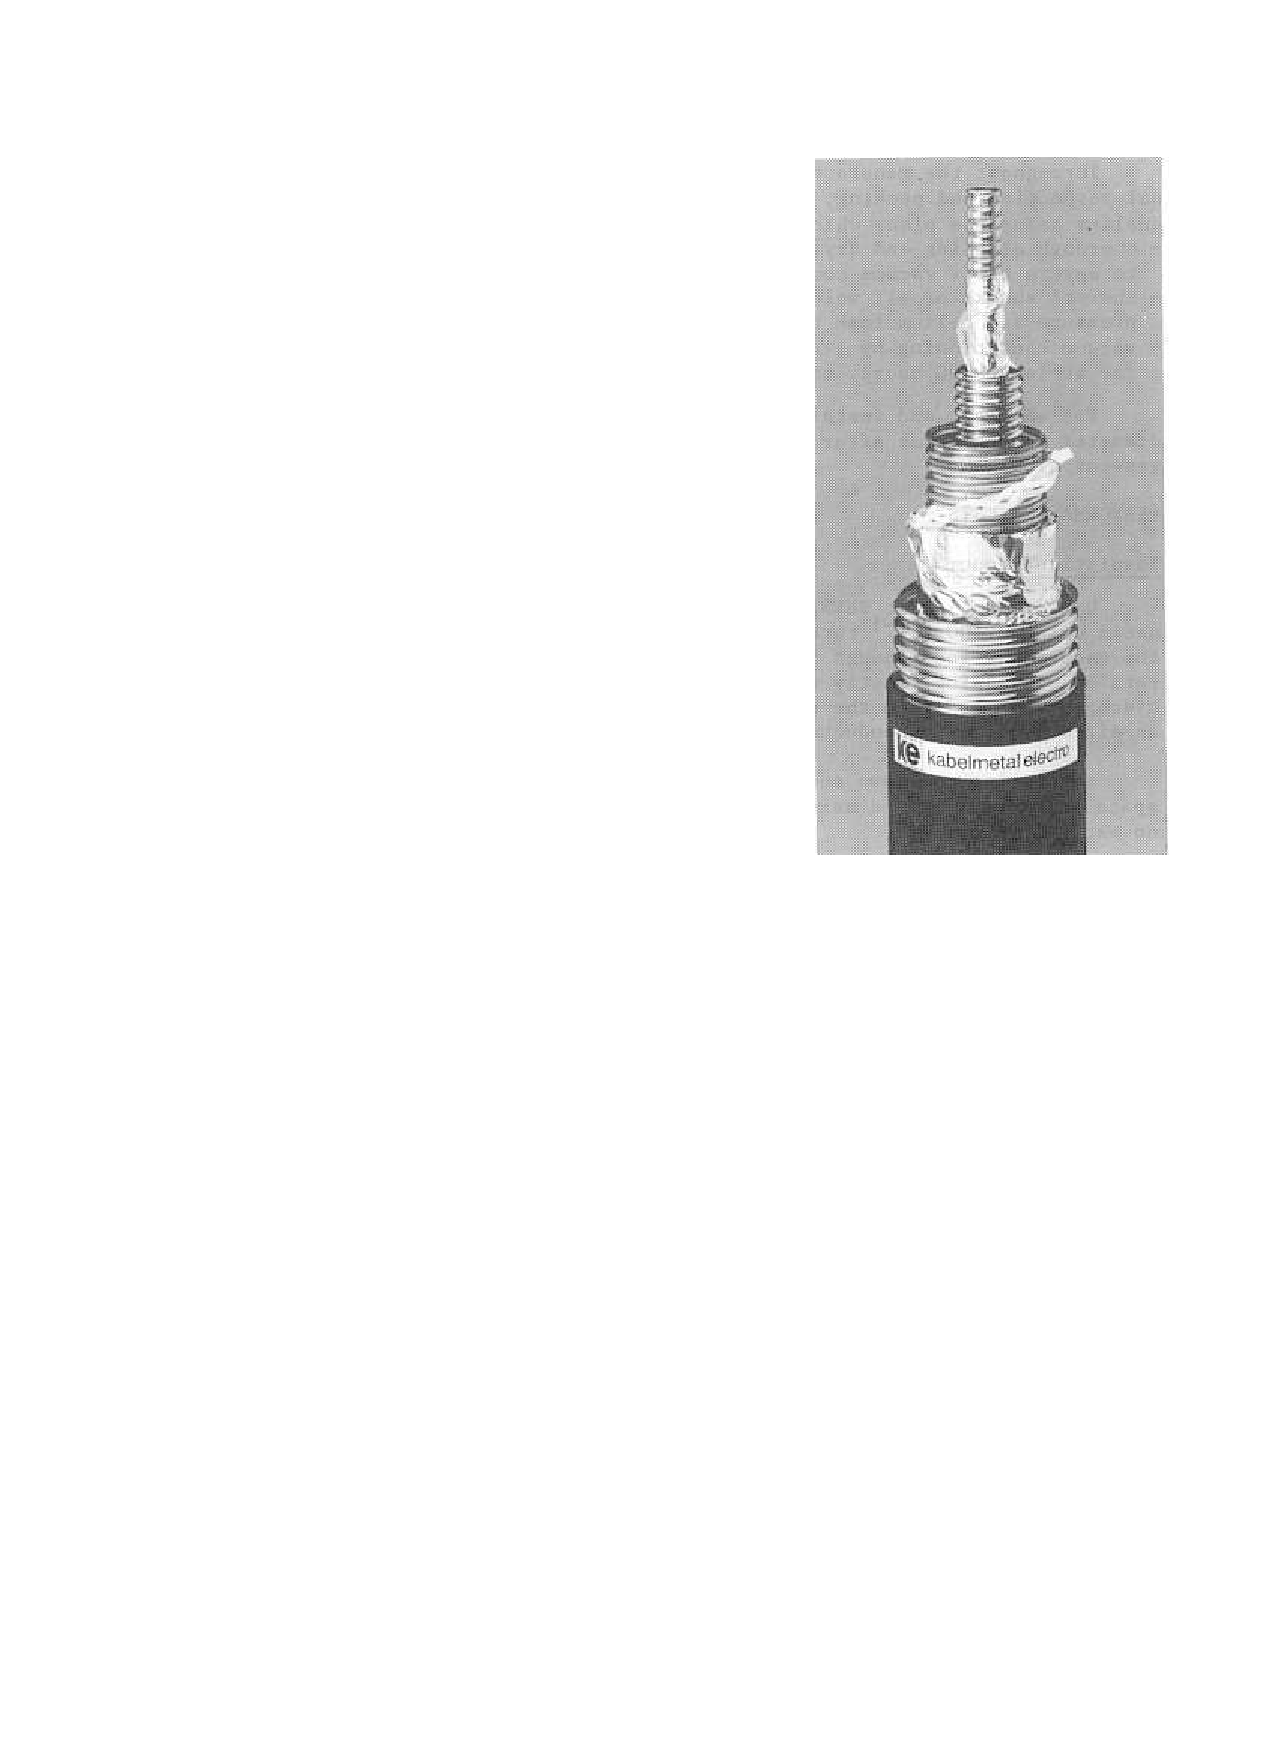
\includegraphics[width=5cm, height=7cm]{Detector/DetFigures/transfer_line.pdf} 
\caption{A cross section of a flexible transfer line developed at CERN in collaboration with Kabel Metalelectro~\cite{Lebrun}} 
\label{fig:transfer_line} 
\end{center} 
\end{figure} 

In order to reduce the quantity of impurities in the helium and to recover the gas, a Purification and Recovery System is implemented in the cryogenic plant. It is composed by a helium vaporizer, a high pressure recovery compressor and a helium cryogenic purifier system. An atmospheric gas bag (100 $m^3$), high pressure containers (20 bottles at 20 MPa, 10 N m$^3$ each) for impure gas helium, 3 medium pressure tanks (30 $m^3$ at 2 MPa) for pure gas helium, a liquid nitrogen container (50,000 L) and dedicated transfer stainless steel pipe lines are provided for the fluids storage. The helium to be recovered is collected in the gas bag; if its temperature is too low to enter in the gas bag, the cold helium is sent to a vaporizer where it is heated to the ambient temperature before entering the helium gas bag. The helium coming from the gas bag is sent to the recovery compressor and stored in the high pressure (20 MPa) bottles from which is delivered to the impure gas storage. The impure gas helium flows to the purifier and then it is stored in medium pressure (up to 2 MPa) pure helium buffers connected to the cycle compressors. The cryoplant will be installed in a building close to the main experiment building on surface. To reduce the noise impact, due to the presence of compressors, a cryogenics compressor hall will be created as a separated part of the technical supplies building. The wall of this hall will be treated by a sound insulation system, to avoid noise transmission between the compressor hall and the other building. 

\subsubsection{Cryogenic plant control}
The cryoplant design and the technical solutions to be adopted are focused on the optimization of the system performances and it will be conceived to implement all the required operative scenarios in a fully automatic mode. 

The facility control system, based on a master/slave architecture, will be split into three plants (each for interferometer vertex ) and three distinct supervisory systems will be provided with engineer and operator workstations. The three control systems will be independent, but inter communication signals will be exchanged among the station units. The internal structure of the cryogenic control system will be based on PLCs (Programmable Logic Controllers), equipment of proven reliability in the industrial environment. A PLC will act as master of the local unit PLCs, with the purpose to coordinate the cryoplant activities and interface the logic unit with the upper subsystem level. Feedback control will be necessary to control for example the speed of the turbines or other parameters like temperature and pressure of the helium in different part of the cryogenic system; since the time constraints are not strict (response times of the order of seconds), the control routines will be executed without problems by PID (Proportional-Integral-Derivative) controllers inside the PLCs. A commercial off-the-shelf Supervisory Control and Data Acquisition system will be employed to monitor the plants, for operator intervention, commissioning, test purposes and data storage. 



\section{Vacuum System}
% author G.Gemme
\label{Sec:Vacuum}
\subsection{Overview and requirements}
\label{Sec:Vacuum:Intro}
In laser interferometers for GW detection the instrument has to be kept under High-Vacuum or Ultra-High-Vacuum (HV, UHV) for several reasons: 
\begin{itemize} 
\item reduce the noise due to vacuum fluctuations along the beam path to an acceptable level; 
\item isolate test masses and other optical elements from acoustic noise; 
\item reduce test mass motion excitation due to residual gas fluctuations;
% \item reduce friction losses in the mirror suspensions %\redcomment{excitation due to residual gas pressure fluctuation and residual gas damping of pendulum motion is the same mechanism}
\item contribute to thermal isolation of test masses and of their support structures; 
\item contribute to preserve the cleanliness of optical elements. 
\end{itemize} 
The power spectral density of gas-induced fluctuations in the optical path length has been calculated choosing conservative beam shape parameters and taking a safety factor of at least $10$ with respect to the pressure producing a phase noise at the limit of the best sensitivity.

The residual gas composition will be dominated by hydrogen with presence of water and other gases; we will keep the total residual pressure at about $10^{-10}$~mbar, corresponding to a noise level below $10^{-25}$~Hz$^{-1/2}$.
The vacuum system will be extremely clean from heavy organic molecules, both to limit the phase noise and to prevent pollution of the optical components. Hydrocarbons partial pressure shall be at the level of $10^{-14}$~mbar.

% \begin{center} 
% \includegraphics{Sec_SiteInfra/Figures/VAC3.jpg} 
% \caption{Phase noise given by the residual gases compared to the expected sensitivity, computed for the appropriate beam profile for different gas compositions. (Goal gas composition: Hydrogen [$1\,10^{-10}$ mbar], Water [$5\,10^{-11}$ mbar], Nitrogen [$1\,10^{-11}$ mbar])} 
% \label{fig:vac3} 
% \end{center} 
% \end{figure} 

To meet these requirements it will be necessary: 
\begin{itemize} 
\item to fire (one week in an air oven at 450$^\circ$C) the stainless steel vacuum enclosure elements (or the raw material sheets) in order to reduce the H$_2$ outgassing rate at the level of $10^{-14}$~mbar~l/cm$^{2}$~s 
\item to bake for one week at $150^\circ$C (or, possibly, at lower temperature) the pipes already assembled and under vacuum in order to eliminate the water molecule layers sticking to the pipe inner wall. 
\end{itemize} 

% Concerning the phase noise, the path length of the beams in HV will be kept short, that is a negligible noise contribution, when compared to the kilometers in the UHV arm pipes. 

The ET vacuum system (Fig. )%\ref{fig:vac1} 
will be composed of several UHV pipes with kilometric length and several cylindrical vertical HV/UHV tanks (towers) containing the optical elements and their support structures (Fig. ).%\ref{fig:vac2}
In general it is necessary to have the whole vacuum system constituting one single volume, without physical separations (windows) on the laser beam path. HV volumes (the towers) contain parts of the apparatus not easily compatible with UHV pipes where, on the contrary, the large majority of the laser beam has to travel. The separation between HV and UHV is obtained by differential pumping or by cryogenic traps, stopping the migration of water and other high vapor pressure components. Large gate valves will be put at each end of the arm pipes, in order to preserve vacuum when venting a tower. For the same reason each tower will be separable from the rest of the vacuum enclosure by suitable gate valves. The filter cavities being less sensitive to vacuum noise require a residual pressure at the level of $10^{-7}$~mbar. Their pipes will neither be fired at 450$^\circ$C nor baked at 150$^\circ$C. 
% \begin{figure} 
% \begin{center} 
% \includegraphics[width=\textwidth]{Sec_SiteInfra/Figures/VAC1.pdf} 
% \caption{Schematic of the ET vacuum system lay-out, out of scale. Only one xylophone detector is shown, out of three.} \label{fig:vac1} 
% \end{center} 
% \end{figure} 

% \begin{figure} 
% \begin{center} 
% \includegraphics[width=0.65\textwidth]{Sec_SiteInfra/Figures/AssNETow2.pdf} 
% \caption{As an example the cross-section of a Virgo a mirror tower is shown.} 
% \label{fig:vac2} 
% \end{center} 
% \end{figure} 

\begin{comment}
The technologies that were developed and employed in the existing gravitational wave observatories have been shown to meet the stringent requirements of vacuum integrity, very low hydrogen and heavy molecule outgassing, minimal particulate generation, low vibration, and appropriate stray light optical absorbance for successful operation. However, straightforward extrapolation of the costs for extending the interferometer vacuum beam enclosures from the current lengths of 3-4~km/arm to $\sim10$~km/arm indicates the need for investigation of a range of technologies and materials that could significantly lower the final cost, facilitate construction and increase the life-cycle operation of vacuum systems for next generation observatories. 
\end{comment}

\subsection{The arm pipes} 
Due to the multi interferometer/xylophone choice for ET, several beams will run along each side of the triangular tunnel. We assume four main beams and two filter cavity beams, taking into account all the three detectors (six interferometers) composing the full ET. 
\redcomment{Has to be consistent with other documents, which state 1\,km filter cavities. }
The chosen baseline configuration includes four pipes, one for each main beam: two with a $0.9$~m diameter for the HF interferometers and two $0.75$~m diameter pipes, for the LF interferometers. In addition, two $0.69$~m pipes for the two filter cavity beams belonging to each LF interferometer. HF interferometers will be equipped also with a $300$~m long filter cavity, running in a dedicated tunnel, inside a $0.6$~m diameter pipe. The pipes will be arranged inside the tunnel cross-section as shown in Fig. 
%\ref{fig:vac4}
: the filter cavities at the bottom, under a movable floor, the two HF beams on the floor at the tunnel sides and the two LF beams on top of them (see below the "Tower" subsection).
%\begin{figure} 
% \begin{center} 
% \includegraphics{Sec_SiteInfra/Figures/VAC4.jpg} \caption{Arrangement of the vacuum pipes in the tunnel cross-section.} 
% \label{fig:vac4} 
% \end{center} 
% \end{figure} 

The pipes will have stainless steel thin walls ($3$--$4$~mm thick) with external stiffening rings, one every $1$--$2$ meters. Two rings will be larger, serving as attachment for the supports (see below). 

$20$~m long pipe elements will be fabricated via industrial tools carefully calculated for large scale economy, logistics optimization and quality assurance. At one end of each element a suitable bellows will be added to accommodate thermal expansion, during bake-out (winter/summer temperature excursion are negligible under ground). At both ends $2$~mm thick lips will be added, to allow UHV compatible welding of adjacent elements, without inert gas protection on the inner side of the weld. 

Simple supports, using steel cables and adjustable stretching screws will be sufficient, coping with the expected stability of the tunnel. 

The pipes will be aligned in the tunnel using optical instruments and laser beams, since GPS will not be applicable under ground. The requested straightness error for the arms is of the order of 10 mm. Periodical surveys will be necessary every few years, in order to detect any pipe displacements due to ground movements. 

Each 10 km pipe will contain a few hundreds of metallic baffles for diffused light mitigation. They shall be made out of stainless steel with a suitable conical shape and serrated inner edge (Fig. %\ref{fig:vac5}
) against diffraction. The radial width of the baffles, between $50$ and $100$~mm, and their position will be determined by a suitable simulation %\cite{vinet97} \cite{vinet96}.
% \begin{figure} 
% \begin{center} 
% \includegraphics{Sec_SiteInfra/Figures/VAC5.jpg} 
% \caption{As an example the Virgo pipe conical baffles are shown.} 
% \label{fig:vac5} 
% \end{center} 
% \end{figure} 

\subsubsection{Pipe Assembly} 
The $20$~m pipe elements will be introduced into the caverns with the ends sealed by suitable end-caps and equipped with thermal insulation; each element will weight about $1.5$~t. The element will be put on and bolted to a simple carriage made of two parallel $20$~m long beams supported by small train wheels. In this way pipe elements can be pushed to their position one after the other by an electric tractor running on $5$~km long rails reaching up to mid arm. The rails, two for each pipe, are supported by frames extending to the whole tunnel cross-section. These same frames have the function, as said before, of supporting the pipes. 

% In alternative the element could be suspended to a $20$ m long beam running, as a bridge crane carriage, on a $5$ km long rail. The rail, one per pipe, is supported by the already mentioned frames. Also in this case pipe elements can be pushed to their position one after the other by an electric tractor or by a traction line. 

Every $500$~m, along the tunnel, there is an enlarged room (``pump room'', Fig.%\ref{fig:VAC7}
) foreseen to host pumping, bake-out and control equipment; those rooms are used also to weld the pipe elements at ease in a wide area, under a mobile clean tent. A pump room is an enlargement of the tunnel for a width of $12$~m and a length of $10$~m, allowing the installation of the pumps, which are hold in their position by a metallic frame not shown in the figure. Three cabinets housing the electronics of the vacuum equipment are included, together with an electrical power supply for baking ($60$~VDC, $300$~kW). A bridge crane shall be present, and the room shall probably need a conditioned humidity and temperature, to allow electronics efficiency. 
% \begin{figure} 
% \begin{center} 
% \includegraphics[width=\textwidth]{Sec_SiteInfra/Figures/VAC7.jpg} 
% \caption{3D view of a pumping station: the blue objects represent the pumps and sensors, the yellow ones the cabinets for pumps control and baking power supply (1 cabinet for all). A separate small room is reserved for the high voltage electrical transformer.} 
% \label{fig:VAC7} 
% \end{center} 
% \end{figure} 

The assembly sequence of a vacuum pipe is described below and is graphically shown in Fig. %\ref{fig:VAC8}. 
% \begin{figure} 
% \begin{center} 
% \includegraphics[width=\textwidth]{Sec_SiteInfra/Figures/VAC8.pdf} 
% \caption{The assembly sequence of one vacuum pipe.} \label{fig:VAC8} 
% \end{center} 
% \end{figure} 

The first pipe element is stopped with the rear end under the tent prepared in the $9^{th}$ pump room, counting from the corner cavern; when the front end of the second element is close, the sealing lids are removed, after starting appropriate clean air flows. The corresponding end lips of the adjacent elements are precisely adjusted and welded. The beams of the two carriages (under or above the pipe, according to the chosen option) are rigidly bolted together, taking care of appropriate compression/extension of the bellows. 

The two modules are shifted forward until the rear end of the second module is at the welding position; now the front end of the third module is adjusted and welded as before. This procedure is continued until the $25^{th}$ module is welded and the $500$~m long section of pipe is completed. 

The $500$~m long section will be then shifted by $20$~m to its final position. 

Every pair of upper support cables are attached to the corresponding support ring, the cables are tightened, the bolts of the pipe elements to the carriages are removed, the elements are lifted by $10$~mm in $1$~mm steps. The $500$~m long train composed by $25$ carriages is sent back to the end cavern, to start the assembly of the second $500$~m pipe section. The lower support cables are attached to the pipe support rings and suitably tightened. 

The ends of the assembled pipe section are closed with vacuum tight lids, the section is evacuated and tightness tests are performed. The closing lids will be strongly fastened to the tunnel wall, in order to keep the 6.4 t axial load due to atmospheric pressure. 

The clean tent and the welding equipment are transferred to the next ($8^{th}$ from the corner cavern) pump room and the assembly of the second $500$ m pipe section is started. Once completed and vacuum tested, taking advantage of the bellows and of the support cables, the front lip of the new $500$ m section and the rear lip of the previous section are connected welding-in a 1 m long junction piece. These final welds are the last to be performed in that particular pump room. 

The procedure continues contemporarily extending the installed pipe from mid arm to both arm ends. 

Concerning the pipes arrangement in the tunnel, it is necessary to have the possibility to inspect and repair the welds between pipe elements. This could be achieved leaving a minimum clearance of about $0.5$~m between the ``nude'' pipes and the tunnel wall (at least every $20$~m). This will be barely sufficient also in the case of small maintenance interventions on the tunnel wall lining. 

\subsubsection{Pipe pumping system} 
The pipe pumping system has been conceived to be composed of standard modules, grouped together, in order to limit the number of pumping stations along the arms. 

The required total residual pressure (hydrogen and other gases) of $10^{-10}$~mbar can be obtained, after firing and bake-out, with one $5000$~l/s pumping group, every $500$~m, both in a $0.9$~m and in a $0.7$~m diameter pipe, the smaller gas load due to the smaller diameter being compensated by the relatively reduced conductance. Below is described the pumping system for one single pipe. 

Each permanent pumping group will consist of three identical modules, each made of one $2500$~l/s Ti sublimation pump (TSP), connected to the pipe through a $250$~mm gate valve (the Ti will be sublimated not in the tube but in a separated chamber), coupled to a $300$~l/s ion pump. The former to pump active gases, the latter to pump inert gases. At such a low pressure TSPs are expected to require not more than one yearly regeneration. NEG (Non Evaporable Getter) pumps are being considered as a possible alternative to TSPs. Some redundancy is necessary to cover the Ti pumps maintenance periods.

Besides the permanent pumping group, every pumping station will include suitable vacuum gauges and two $2000$~l/s turbo, backed by a dry pump, for initial evacuation and bake-out. 

The filter cavity pipes, requiring a $10^{-7}$~mbar residual pressure, will be equipped only with the turbo/scroll groups, possibly reinforced with $77$~K cryo-pumps. Ion pumps could also be taken into consideration, for their ease of operation and low noise characteristics, eventually equipped with proper shields to limit risks of charged particles emissions. To meet these specifications, the bake-out will not be necessary, hence filter pipes will not be equipped with thermal insulation.

Every $10$~km pipe will have three residual gas analysers (RGA), at each end and in the middle, to monitor the vacuum quality and for easier diagnosis in case of problems.

\subsubsection{Pipe bake-out system} 
In order to perform the 10-days bake-out under vacuum at 150$^{\circ}$C, the pipe will be heated by electrical current flowing in its walls, closing the circuit by a suitable Al bar or cable. The use of DC will assure a uniform current and temperature distribution on the pipe walls and improve human safety. Typical arrangement of the circuit could be a series of double ring circuits with one DC source every $500$~m delivering $1000$~A at $50$~V along $250$~m in each direction. This system will deliver $200$~W per meter of pipe, which has been experimentally demonstrated to be sufficient to reach 150$^{\circ}$C, if the pipe is wrapped in a suitable $10$--$20$~cm thick thermal insulation layer. Each DC source will consist of a transformer/rectifier supplied by medium voltage AC ($15$~kV). This choice is dictated to reduce the cross section of cables to distribute $2$~MW along $10$~km. $15$~kV equipment will be confined in dedicated rooms. 

In this configuration, delivering $300$~W per meter of tunnel, in absence of ventilation, a very crude estimate considering a $6$~m aperture tunnel, drilled in isotropic rocks -- assumed $\rho = 2500$~kg/m$^{3}$, $k = 2.0$~watt/(m K), $C = 800$~joule/(kg K) -- gives an increase of room and wall temperature by about +13$^{\circ}$C after a $10$~days bake-out. This situation, being at the limit of what could be tolerable, suggests to exploit several remedies, like baking at a lower temperature for more days and improving the thermal insulation properties, in order to reduce the temperature increase of the tunnel walls. A suitable air cooling system will be designed to reduce further the ambient temperature (possibly renewing once per hour the tunnel air volume). The overall power release inside the tunnel could be reduced also performing bake-out in sequence on shorter pipe sections, separated by ``pseudo-valves'', vacuum tight, but able to sustain merely null pressure difference.

\subsection{Cryotraps} 
HV volumes (e.g. the towers) will communicate with the UHV pipe through liquid nitrogen cryotraps, to prevent migration of water and other high vapor pressure contaminants. In order to allow the beam passage, the cryotraps will consist of a large hollow muff, containing liquid nitrogen, suspended inside an increased diameter pipe section, with a design very similar to the one adopted for LIGO, Virgo and Advanced Virgo (Fig. %\ref{fig:vac6}
). 

The lateral surface will be thermally isolated by a few cylindrical metal screens; the heat exchange at both ends will be limited by circular baffles, leaving passage for the beam. The propagation of mechanical noise due to liquid nitrogen bubbling will be limited installing cryotraps at least $20$~m away from the mirror towers. 

Cryotraps will have valves at each end, in order to be confined during warming-up for regeneration (not more than once per year). 

The traps will be $7$--$10$~m long for pipes with diameters of $0.6$--$1.0$~m. The liquid nitrogen consumption has been evaluated to be about 10 liters per hour per trap. 

In correspondence of the cryogenic towers for the $10$~K mirrors of the LF interferometer, the cryotraps will be much longer ($50$~m) and will include liquid helium sections to strongly limit the mirror heat exchange as described in the following section. We refer to the same section for a description of the supply plant for cryogenic liquids. 
% \begin{figure} 
% \begin{center} 
% \includegraphics{Sec_SiteInfra/Figures/VAC6.jpg} 
% \caption{A liquid nitrogen cryotrap.} 
% \label{fig:vac6} 
% \end{center} 
% \end{figure} 

\subsection{Towers}
The upper part of the mirror towers will have a $2$--$3$~m diameter to contain easily the pendulum chains of Superattenuators and the inverted pendulum legs; the structure will be an evolution of the Virgo towers (Fig. %\ref{fig:vac2}
). The lower chamber of the towers will have a diameter up to $3$~m, to contain large payloads. 

The HF interferometer towers will have a large bottom lid to allow installation of payloads from a clean basement, under a filtered air shower. The height will be $10$~m for the main mirrors of the warm HF interferometer. Auxiliary mirrors or benches requiring lower isolation, will be located in shorter towers. 

The towers containing the cryogenic mirrors of the LF interferometer, to achieve full seismic isolation performance down to $2$~Hz, will be up to $20$~m tall. In these towers, sitting on top of the HF interferometer, the payload installation will be performed through a lateral port. This order of superposition has been chosen to have the low power LF beam passing through the HF mirror suspensions (at room temperature) and not the high power HF beam passing through the low temperature LF mirror suspensions. The lower part of the cryogenic towers will be described in the next section. 

Each cryo-tower will be coupled to an ancillary tower to support the heat extraction chain preventing seismic noise propagation. 

\subsubsection{Tower pumping system} 
The towers will be made of two or three vacuum compartments in order to separate by differential vacuum the lower mirror chamber from the less clean suspension mechanics in the upper chamber. The horizontal separating walls will have a low conductance hole for the passage of the pendulum chain support wire. 

The mirror chamber will be equipped with a permanent pumping group consisting of one $2500$~l/s Ti sublimation pump coupled to a $300$~l/s ion pump. In addition one $2000$~l/s turbo, backed by a scroll pump, will be operated for initial evacuation. 

The tower upper chamber(s) will be pumped by suitable turbo/scroll groups. An effort will be performed to build the suspension mechanics and electronics with ultra clean and low outgassing components, in order to pump permanently also the upper chamber with ion pumps. 

The use of large cryo-pumps is being considered to increase pumping power and to eliminate moving parts from the vicinity of mirrors. 

\subsection{Valves} 
A great number of UHV gate valves with large aperture, up to 1 m will be necessary. They will be all metal with only the gate gasket out of vacuum outgassed Viton. 

Every tower will be separable from the rest of the vacuum system by such valves. Every cryotrap will also be separable for regeneration; the HV side will be equipped with a Viton gasket valve, while the UHV side will be equipped with a totally metallic ``pseudo valve'', vacuum tight, but tolerating only a few mbar pressure difference.


